\pdfminorversion=4 % for acroread
\documentclass[t,xcolor={usenames,dvipsnames}]{beamer}
%\documentclass[t,handout,xcolor={usenames,dvipsnames}]{beamer}
\usepackage{beamerstyle}
\usepackage{dsfont}
\usepackage{bm}
\usepackage[english]{babel}
\usepackage[utf8]{inputenc}
\usepackage{graphicx}
\usepackage[boxed,vlined]{algorithm2e}
\usepackage{hyperref}
\usepackage{booktabs}

\usepackage{amsmath,amssymb}
\usepackage{listings}
\lstset{frame=lines,framesep=3pt,numbers=left,numberblanklines=false,basicstyle=\ttfamily\small}

\usepackage{subfig}
\usepackage{multicol}
%\usepackage{appendixnumberbeamer}
%
\newcommand{\votepurple}[1]{\textcolor{Purple}{$\bigstar$}}
\newcommand{\voteyellow}[1]{\textcolor{Goldenrod}{$\bigstar$}}
\newcommand{\voteblue}[1]{\textcolor{RoyalBlue}{$\bigstar$}}
\newcommand{\votepink}[1]{\textcolor{Pink}{$\bigstar$}}

\newcommand{\refstyle}[1]{{\small{\textcolor{gray}{#1}}}}
\newcommand{\hands}[0]{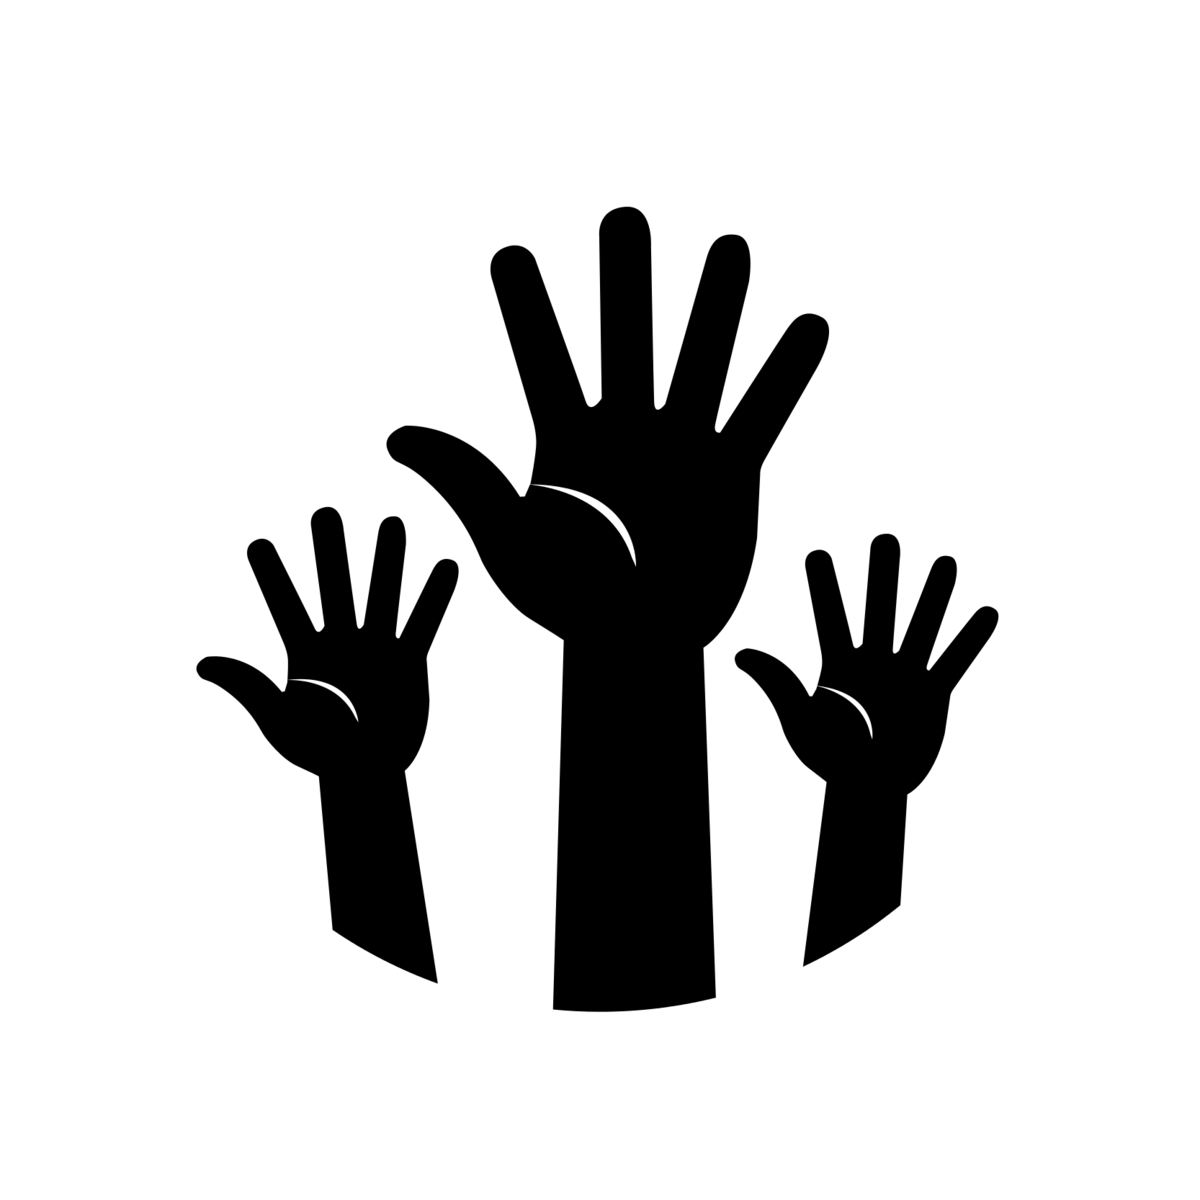
\includegraphics[height=1.5em]{images/hands}}

\newcommand\transpose{{\textrm{\tiny{\sf{T}}}}}

\usepackage{tikz}
\usetikzlibrary{trees} 
\usetikzlibrary{shapes.geometric}
\usetikzlibrary{positioning,shapes,shadows,arrows,calc,mindmap}
\usetikzlibrary{decorations.pathreplacing}
\usetikzlibrary{intersections}
\pgfdeclarelayer{background}
\pgfdeclarelayer{foreground}
\pgfsetlayers{background,main,foreground}
\tikzstyle{activity}=[rectangle, draw=black, rounded corners, text centered, text width=8em]
\tikzstyle{data}=[rectangle, draw=black, text centered, text width=8em]
\tikzstyle{myarrow}=[->, thick, draw=black]

% Define the layers to draw the diagram
\pgfdeclarelayer{background}
\pgfdeclarelayer{foreground}
\pgfsetlayers{background,main,foreground}
\newcommand{\myit}[1]{\begin{itemize}#1\end{itemize}}
\newcommand{\cplex}[0]{CPLEX}
\newcommand{\lpsolve}[0]{lpsolve}
\newcommand{\gurobi}[0]{Gurobi}


%\usepackage{listings}
%\lstset{numbers=left,
%  showstringspaces=false,
%  frame={tb},
%  captionpos=b,
%  lineskip=0pt,
%  basicstyle=\ttfamily,
%%  extendedchars=true,
%  stepnumber=1,
%  numberstyle=\small,
%  xleftmargin=1em,
%  breaklines
%}

 

\usetheme{Madrid}
%\useinnertheme{rectangles}
\usecolortheme{whale}
\setbeamercolor{alerted text}{fg=blue}
\useoutertheme{infolines}
\setbeamertemplate{navigation symbols}{\vspace{-5pt}} % to lower the logo
\setbeamercovered{invisible}

\makeatletter
\setbeamertemplate{footline}
{
  \leavevmode%
  \hbox{%
  \begin{beamercolorbox}[wd=.333333\paperwidth,ht=2.25ex,dp=1ex,center]{author in head/foot}%
    \usebeamerfont{author in head/foot}\insertshortauthor
  \end{beamercolorbox}%
  \begin{beamercolorbox}[wd=.333333\paperwidth,ht=2.25ex,dp=1ex,center]{title in head/foot}%
    \usebeamerfont{title in head/foot}\insertshorttitle
  \end{beamercolorbox}%
  \begin{beamercolorbox}[wd=.333333\paperwidth,ht=2.25ex,dp=1ex,right]{date in head/foot}%
    \usebeamerfont{date in head/foot}\insertshortdate{}\hspace*{2em}
    \insertframenumber\hspace*{2ex} 
  \end{beamercolorbox}}%
  \vskip0pt%
}
\makeatother

\newcommand{\lit}[1]{{\footnotesize\color{black!70}[#1]}}
\newcommand{\litw}[1]{{\footnotesize\color{black!20}[#1]}}

\pgfdeclareimage[height=1.2cm]{coseallogo}{images/logos/coseal}
\pgfdeclareimage[height=1.2cm]{mlaad}{images/logos/ml4aad.png}
\pgfdeclareimage[height=1.2cm]{freiburg}{images/logos/freiburg}

\logo{\pgfuseimage{freiburg}}

\title[ML4AAD]{Machine Learning for Automated Algorithm Design}
\subtitle{(ML4AAD)}
\author{M. Lindauer \and A. Biedenkapp}
\institute{University of Freiburg\\[5em]
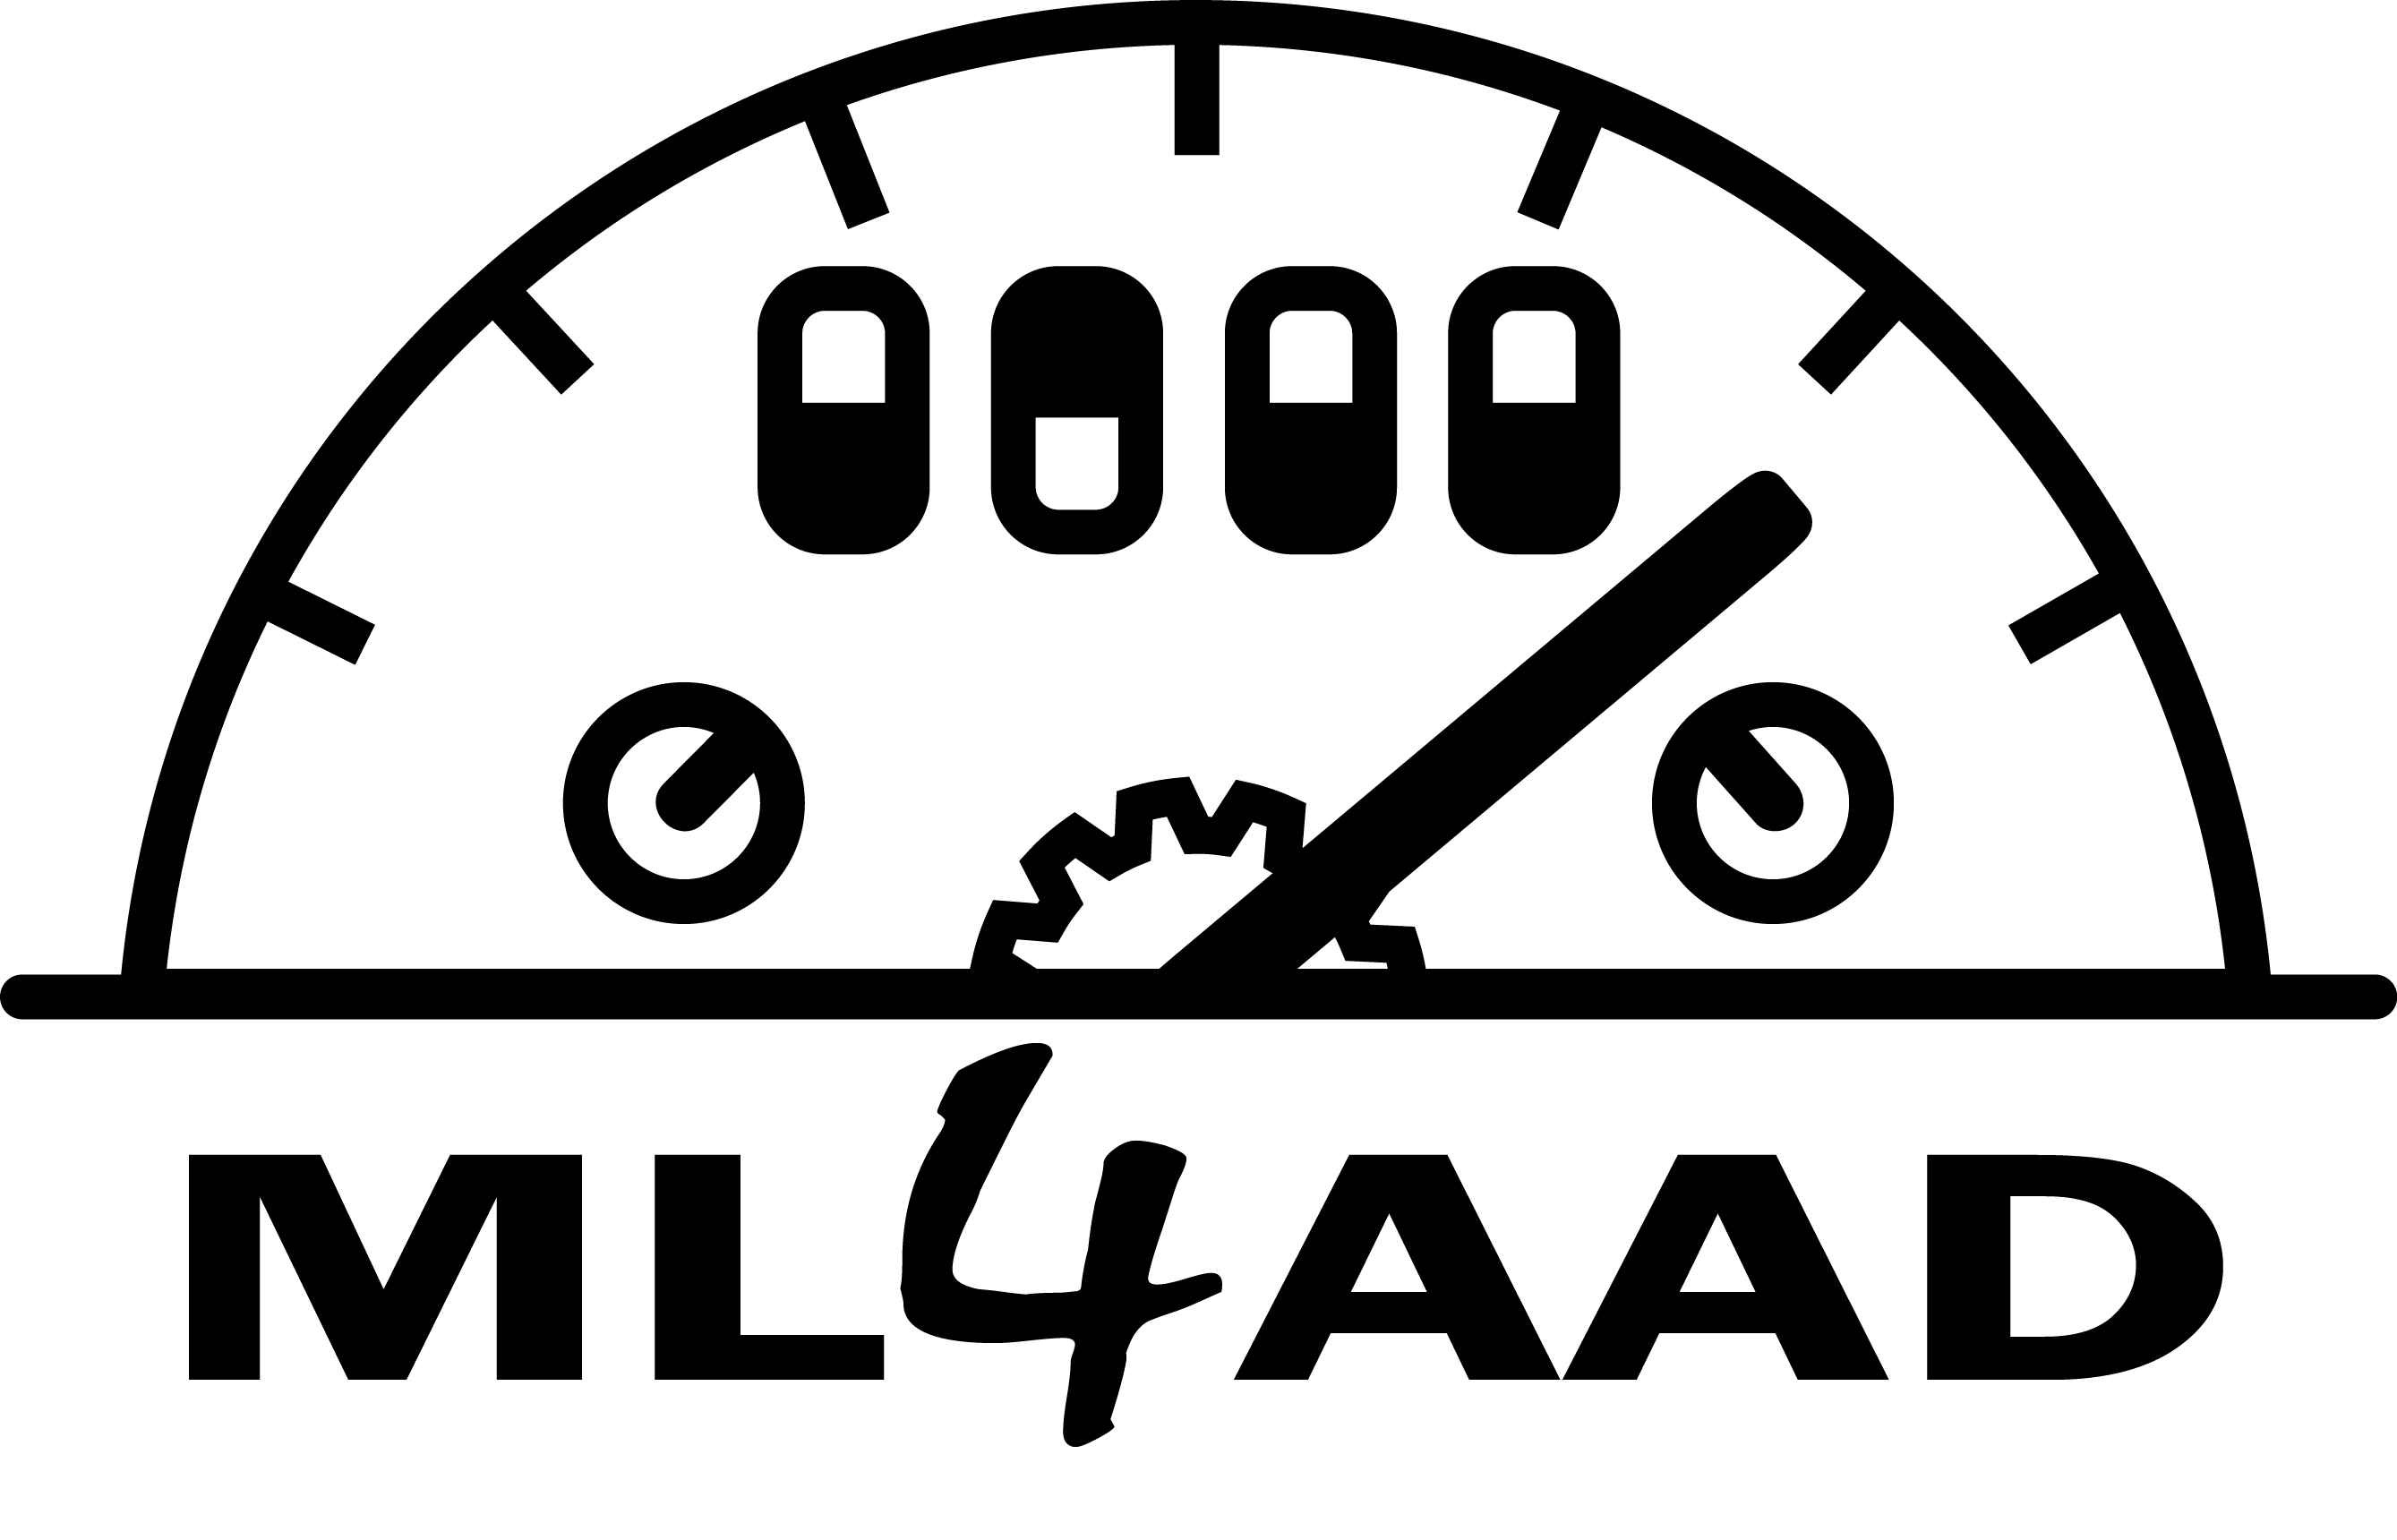
\includegraphics[width=10em]{images/ml4aad}}
\date{}



% \AtBeginSection[] % Do nothing for \section*
% {
%   \begin{frame}{Outline}
%     \bigskip
%     \vfill
%     \tableofcontents[currentsection]
%   \end{frame}
% }

\renewcommand{\comment}[1]{
	\noindent
	%\vspace{0.25cm}
	{\color{red}{\textbf{TODO:} #1}}
	%\vspace{0.25cm}
}
\newcommand{\notefh}[1]{\textcolor{red}{\textbf{FH:} #1}}
\renewcommand{\comment}[1]{}
\newcommand{\hide}[1]{}
\newcommand{\cemph}[2]{\emph{\textcolor{#1}{#2}}}

\newcommand{\lit}[1]{{\footnotesize\color{black!60}[#1]}}

\newcommand{\litw}[1]{{\footnotesize\color{blue!20}[#1]}}


\newcommand{\myframe}[2]{\begin{frame}[c]{#1}#2\end{frame}}
\newcommand{\myframetop}[2]{\begin{frame}{#1}#2\end{frame}}
\newcommand{\myit}[1]{\begin{itemize}#1\end{itemize}}
\newcommand{\myblock}[2]{\begin{block}{#1}#2\end{block}}


\newcommand{\votepurple}[1]{\textcolor{Purple}{$\bigstar$}}
\newcommand{\voteyellow}[1]{\textcolor{Goldenrod}{$\bigstar$}}
\newcommand{\voteblue}[1]{\textcolor{RoyalBlue}{$\bigstar$}}
\newcommand{\votepink}[1]{\textcolor{Pink}{$\bigstar$}}

\newcommand{\diff}{\mathop{}\!\mathrm{d}}
\newcommand{\refstyle}[1]{{\small{\textcolor{gray}{#1}}}}
\newcommand{\hands}[0]{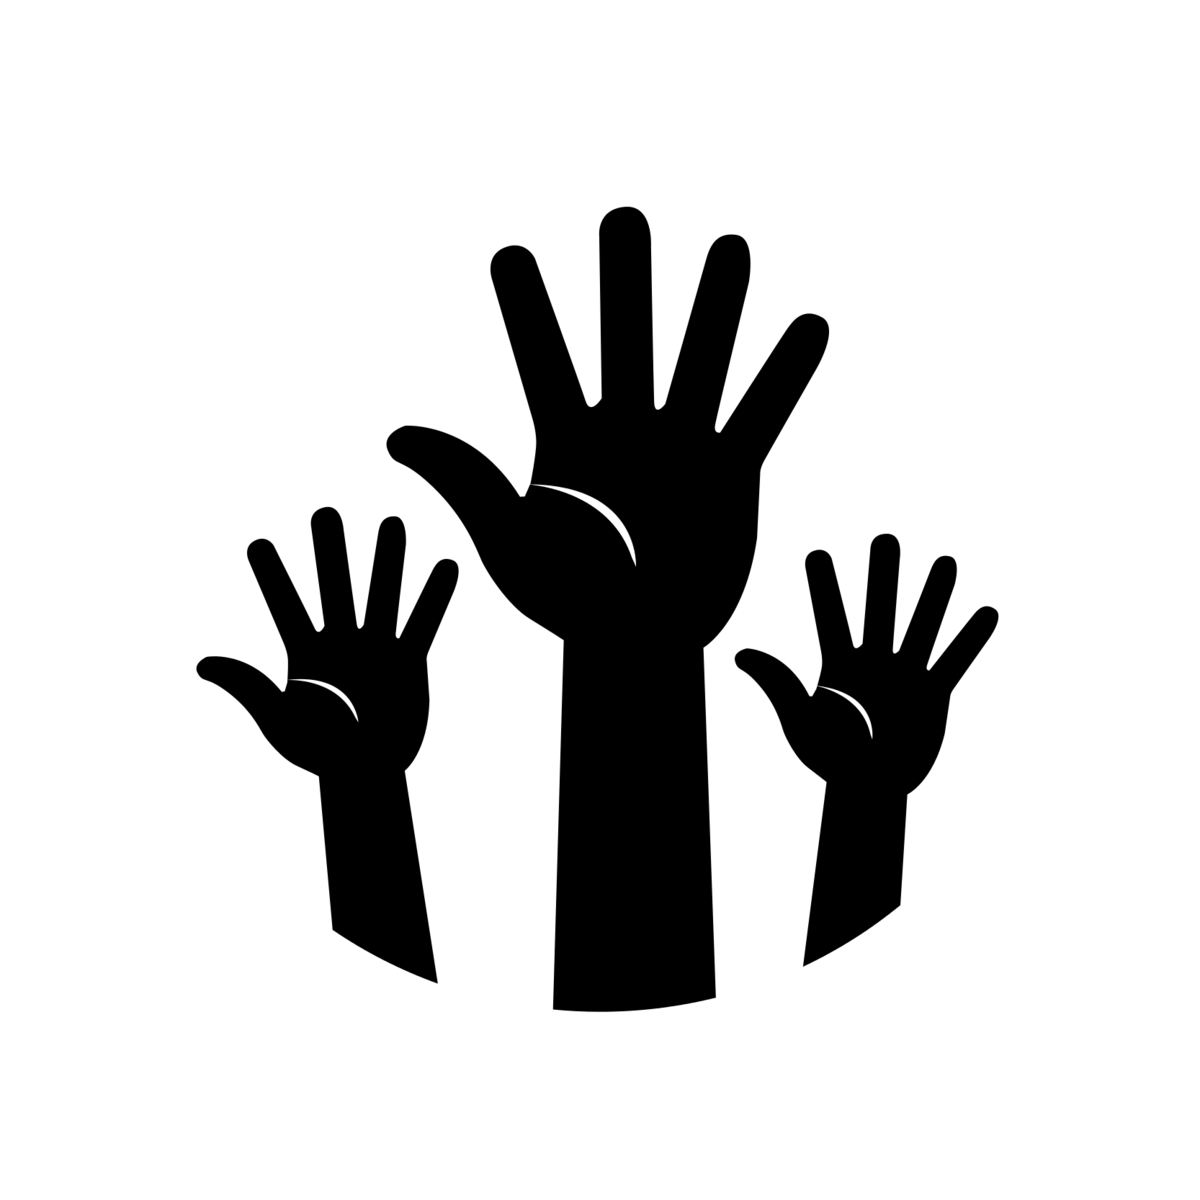
\includegraphics[height=1.5em]{images/hands}}
\newcommand{\transpose}[0]{{\textrm{\tiny{\sf{T}}}}}
\newcommand{\norm}{{\mathcal{N}}}
\newcommand{\cutoff}[0]{\kappa}
\newcommand{\instD}[0]{\dataset}
\newcommand{\insts}[0]{\mathcal{I}}
\newcommand{\inst}[0]{i}
\newcommand{\instI}[1]{i^{(#1)}}

% Iteration specific instance of variable/function/anything
% Introduced in the BO section, but moved up here to make it available within other macros
\newcommand{\iter}[2][\bocount]{{#2}^{(#1)}}

%--------HPO parameter macros-----------

% Parameter Configuration Space
\newcommand{\pcs}[0]{\pmb{\Lambda}}

% ???
\newcommand{\bx}[0]{\conf}

% Parameter Configuration
\newcommand{\conf}[0]{\pmb{\lambda}}

% Final Configuration
\newcommand{\finconf}[0]{\pmb{\hat{\lambda}}}

% Configuration corresponding to a given iteration -- better use \iter!
\newcommand{\confI}[1]{{\conf}^{(#1)}}

% Default Configuration
\newcommand{\defconf}[0]{{\conf}_{\text{def}}}

% Incumbent Configuration
\newcommand{\incumbent}[1][\bocount]{\iter[#1]{\finconf}}

% Optimal Configuration
\newcommand{\optconf}[0]{{\conf}^*}

% Configuration Space
\newcommand{\confs}[0]{\pcs}

%----------------------------------------

%\newcommand{\vlambda}[0]{\bm{\lambda}}
%\newcommand{\vLambda}[0]{\bm{\Lambda}}
\newcommand{\dataset}[0]{\mathcal{D}}
\newcommand{\datasets}[0]{\mathbf{D}}
\newcommand{\loss}[0]{L}
\newcommand{\risk}{\mathcal{R}}
\newcommand{\riske}{\mathcal{R}_{\text{emp}}}
\newcommand{\cost}[0]{c}
\newcommand{\costI}[1]{c^{(#1)}}

% Gaussian Process
\newcommand{\gp}{\mathcal{G}}
% Family of Objective Functions
\newcommand{\objF}{F}

%---------------BO Macros------------------

% BO loop counter
\newcommand{\bocount}{t}
% BO loop counter max, the counter runs from 1 to this value
\newcommand{\bobudget}{T}
% BO loop observation
\newcommand{\obs}[1][\conf]{\cost({#1})}
% BO loop observation space
\newcommand{\obsspace}{\mathcal{Y}}
% BO loop next observation
\newcommand{\bonextobs}{\obs[\iter{\conf}]}
% Acquisition Function, no args
\newcommand{\acq}{u}
% Standard Normal PDF
\newcommand{\pdf}{\phi}
% Standard Normal CDF
\newcommand{\cdf}{\Phi}
% Mean
\newcommand{\mean}{\mu}
% Standard Deviation
\newcommand{\stddev}{\sigma}
% Variance
\newcommand{\variance}{\sigma^2}
% Noise
\newcommand{\noise}{\nu}
% BO loop next selected sample
\newcommand{\bonextsample}{\confI{\bocount}}

% Single hyperparameter
\newcommand{\hyperparam}{\lambda}

% Single hyperparameter within a hyperparameter configuration
\newcommand{\hyperparami}[1][i]{{\hyperparam}_#1}

% Full definition of final configuration
\newcommand{\finconffull}{\incumbent[\bobudget]}

% Dataset
\newcommand{\datasetHPO}{{\dataset}_{HPO}}

% Dataset definition
\newcommand{\datasetHPOdef}{{\langle \bonextsample,\,\bonextobs \rangle}_{\bocount=1}^{\bobudget}}

% Double Display Fraction, forces large displays for everything in numerator and denominator
\newcommand\ddfrac[2]{\frac{\displaystyle #1}{\displaystyle #2}}

% Conditional Probability "Given That" Relation, source:https://tex.stackexchange.com/a/141685/205886
\newcommand\given[1][]{\:#1\vert\:}

% Expectation as a math operator
\DeclareMathOperator*{\E}{\mathbb{E}}

% Citation 
\newcommand{\source}[1]{
    \begin{flushright}
    	Source: \lit{#1}
    \end{flushright}
}
%-------------------------------------------

%Real numbers set
\newcommand{\realnum}{\mathbb{R}}
%Configuration space - do not use
%\newcommand{\configspace}{\Theta}
%Instances - do not use
%\newcommand{\instances}{\mathcal{I}}
%Expected value
\newcommand{\expectation}{\mathbb{E}}
%Kernel
\newcommand{\kernel}{\kappa}
%Constraint function
\newcommand{\constraintf}{c}
%Normal distribution
\newcommand{\normaldist}{\mathcal{N}}

% \renewcommand{\vec}[1]{\mathbf{#1}}
\newcommand{\hist}[0]{\dataset_{\text{Hist}}}
\newcommand{\param}[0]{p}
\newcommand{\algo}[0]{\mathcal{A}}
\newcommand{\algos}[0]{\mathbf{A}}
%\newcommand{\nn}[0]{N}
\newcommand{\feats}[0]{\mathcal{X}_{\text{meta}}}
\newcommand{\feat}[0]{\x_{\text{meta}}}
%\newcommand{\cluster}[0]{\vec{h}}
%\newcommand{\clusters}[0]{\vec{H}}
\newcommand{\perf}[0]{\mathbb{R}}
%\newcommand{\surro}[0]{\mathcal{S}}
\newcommand{\surro}[0]{\hat{\cost}}
\newcommand{\func}[0]{f}
\newcommand{\epm}[0]{\surro}
\newcommand{\portfolio}[0]{\mathbf{P}}
\newcommand{\schedule}[0]{\mathcal{S}}

% Machine Learning
\newcommand{\mdata}[0]{\dataset_{\text{meta}}}
\newcommand{\datasettrain}[0]{\dataset_{\text{train}}}
\newcommand{\datasetval}[0]{\dataset_{\text{val}}}
\newcommand{\datasettest}[0]{\dataset_{\text{test}}}
\newcommand{\x}[0]{\mathbf{x}}
\newcommand{\y}[0]{y}
\newcommand{\xI}[1]{\mathbf{x}^{(#1)}}
\newcommand{\yI}[1]{y^{(#1)}}
\newcommand{\fx}{f(\mathbf{x})}  % f(x), continuous prediction function
\newcommand{\Hspace}{\mathcal{H}} % hypothesis space where f is from
\newcommand{\fh}{\hat{f}}       % f hat, estimated prediction function

% Deep Learning
\newcommand{\weights}[0]{\theta}
\newcommand{\metaweights}[0]{\phi}


% reinforcement learning
\newcommand{\policies}[0]{\mathbf{\Pi}}
\newcommand{\policy}[0]{\pi}
\newcommand{\actionRL}[0]{a}
\newcommand{\stateRL}[0]{s}
\newcommand{\statesRL}[0]{\mathcal{S}}
\newcommand{\rewardRL}[0]{r}
\newcommand{\rewardfuncRL}[0]{\mathcal{R}}

\RestyleAlgo{algoruled}
\DontPrintSemicolon
\LinesNumbered
\SetAlgoVlined
\SetFuncSty{textsc}

\SetKwInOut{Input}{Input}
\SetKwInOut{Output}{Output}
\SetKw{Return}{return}

%\newcommand{\changed}[1]{{\color{red}#1}}

%\newcommand{\citeN}[1]{\citeauthor{#1}~(\citeyear{#1})}

\renewcommand{\vec}[1]{\mathbf{#1}}
\DeclareMathOperator*{\argmin}{arg\,min}
\DeclareMathOperator*{\argmax}{arg\,max}

%\newcommand{\aqme}{\textit{AQME}}
%\newcommand{\aslib}{\textit{ASlib}}
%\newcommand{\llama}{\textit{LLAMA}}
%\newcommand{\satzilla}{\textit{SATzilla}}
%\newcommand{\satzillaY}[1]{\textit{SATzilla'{#1}}}
%\newcommand{\snnap}{\textit{SNNAP}}
%\newcommand{\claspfolioTwo}{\textit{claspfolio~2}}
%\newcommand{\flexfolio}{\textit{FlexFolio}}
%\newcommand{\claspfolioOne}{\textit{claspfolio~1}}
%\newcommand{\isac}{\textit{ISAC}}
%\newcommand{\eisac}{\textit{EISAC}}
%\newcommand{\sss}{\textit{3S}}
%\newcommand{\sunny}{\textit{Sunny}}
%\newcommand{\ssspar}{\textit{3Spar}}
%\newcommand{\cshc}{\textit{CSHC}}
%\newcommand{\cshcpar}{\textit{CSHCpar}}
%\newcommand{\measp}{\textit{ME-ASP}}
%\newcommand{\aspeed}{\textit{aspeed}}
%\newcommand{\autofolio}{\textit{AutoFolio}}
%\newcommand{\cedalion}{\textit{Cedalion}}
\newcommand{\fanova}{\textit{fANOVA}}
\newcommand{\sbs}{\textit{SB}}
\newcommand{\oracle}{\textit{VBS}}

% like approaches
\newcommand{\claspfoliolike}[1]{\texttt{claspfolio-#1-like}}
\newcommand{\satzillalike}[1]{\texttt{SATzilla'#1-like}}
\newcommand{\isaclike}{\texttt{ISAC-like}}
\newcommand{\ssslike}{\texttt{3S-like}}
\newcommand{\measplike}{\texttt{ME-ASP-like}}

\newcommand{\irace}{\textit{I/F-race}}
\newcommand{\gga}{\textit{GGA}}
\newcommand{\smac}{\textit{SMAC}}
\newcommand{\paramils}{\textit{ParamILS}}
\newcommand{\spearmint}{\textit{Spearmint}}
\newcommand{\tpe}{\textit{TPE}}


\usepackage{pifont}
\newcommand{\itarrow}{\mbox{\Pisymbol{pzd}{229}}}
\newcommand{\ithook}{\mbox{\Pisymbol{pzd}{52}}}
\newcommand{\itcross}{\mbox{\Pisymbol{pzd}{56}}}
\newcommand{\ithand}{\mbox{\raisebox{-1pt}{\Pisymbol{pzd}{43}}}}

%\DeclareMathOperator*{\argmax}{arg\,max}

\newcommand{\ie}{{\it{}i.e.\/}}
\newcommand{\eg}{{\it{}e.g.\/}}
\newcommand{\cf}{{\it{}cf.\/}}
\newcommand{\wrt}{\mbox{w.r.t.}}
\newcommand{\vs}{{\it{}vs\/}}
\newcommand{\vsp}{{\it{}vs\/}}
\newcommand{\etc}{{\copyedit{etc.}}}
\newcommand{\etal}{{\it{}et al.\/}}

\newcommand{\pscProc}{{\bf procedure}}
\newcommand{\pscBegin}{{\bf begin}}
\newcommand{\pscEnd}{{\bf end}}
\newcommand{\pscEndIf}{{\bf endif}}
\newcommand{\pscFor}{{\bf for}}
\newcommand{\pscEach}{{\bf each}}
\newcommand{\pscThen}{{\bf then}}
\newcommand{\pscElse}{{\bf else}}
\newcommand{\pscWhile}{{\bf while}}
\newcommand{\pscIf}{{\bf if}}
\newcommand{\pscRepeat}{{\bf repeat}}
\newcommand{\pscUntil}{{\bf until}}
\newcommand{\pscWithProb}{{\bf with probability}}
\newcommand{\pscOtherwise}{{\bf otherwise}}
\newcommand{\pscDo}{{\bf do}}
\newcommand{\pscTo}{{\bf to}}
\newcommand{\pscOr}{{\bf or}}
\newcommand{\pscAnd}{{\bf and}}
\newcommand{\pscNot}{{\bf not}}
\newcommand{\pscFalse}{{\bf false}}
\newcommand{\pscEachElOf}{{\bf each element of}}
\newcommand{\pscReturn}{{\bf return}}

%\newcommand{\param}[1]{{\sl{}#1}}
\newcommand{\var}[1]{{\it{}#1}}
\newcommand{\cond}[1]{{\sf{}#1}}
%\newcommand{\state}[1]{{\sf{}#1}}
%\newcommand{\func}[1]{{\sl{}#1}}
\newcommand{\set}[1]{{\Bbb #1}}
%\newcommand{\inst}[1]{{\tt{}#1}}
\newcommand{\myurl}[1]{{\small\sf #1}}

\newcommand{\Nats}{{\Bbb N}}
\newcommand{\Reals}{{\Bbb R}}
\newcommand{\extset}[2]{\{#1 \; | \; #2\}}

\newcommand{\vbar}{$\,\;|$\hspace*{-1em}\raisebox{-0.3mm}{$\,\;\;|$}}
\newcommand{\vendbar}{\raisebox{+0.4mm}{$\,\;|$}}
\newcommand{\vend}{$\,\:\lfloor$}


\newcommand{\goleft}[2][.7]{\parbox[t]{#1\linewidth}{\strut\raggedright #2\strut}}
\newcommand{\rightimage}[2][.3]{\mbox{}\hfill\raisebox{1em-\height}[0pt][0pt]{\includegraphics[width=#1\linewidth]{#2}}\vspace*{-\baselineskip}}

\usepackage{mathtools}

\begin{document}

\maketitle

\newcommand{\mypause}[0]{\pause}
\renewcommand{\mypause}[0]{}

%\begin{frame}[c]{In a Nutshell}

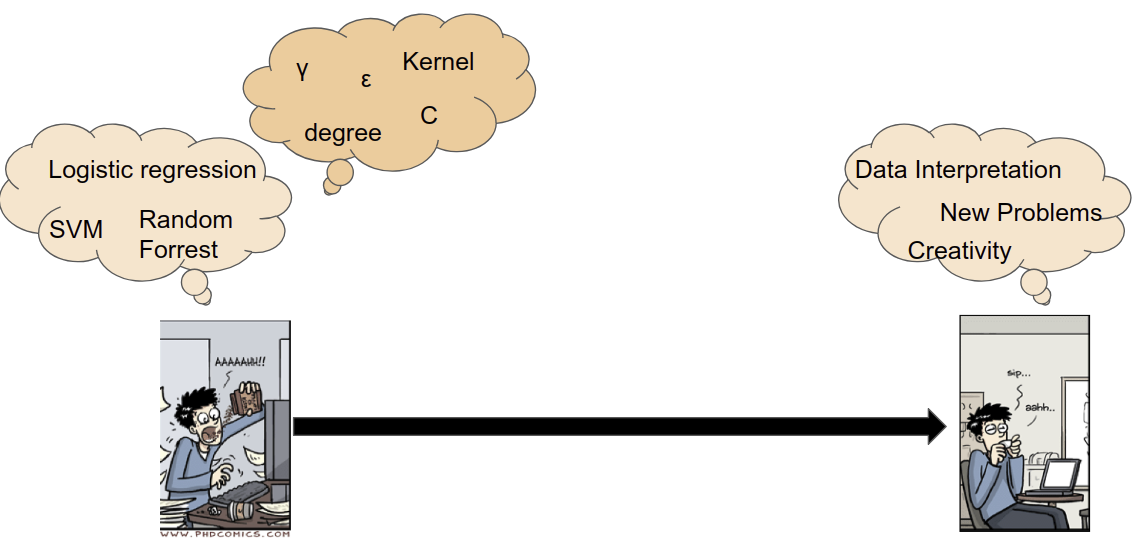
\includegraphics[width=0.99\textwidth]{images/automl_comic}

\end{frame}
%----------------------------------------------------------------------
%----------------------------------------------------------------------
\begin{frame}[c]{}

\huge
\centering
Why are you sitting here?

\bigskip

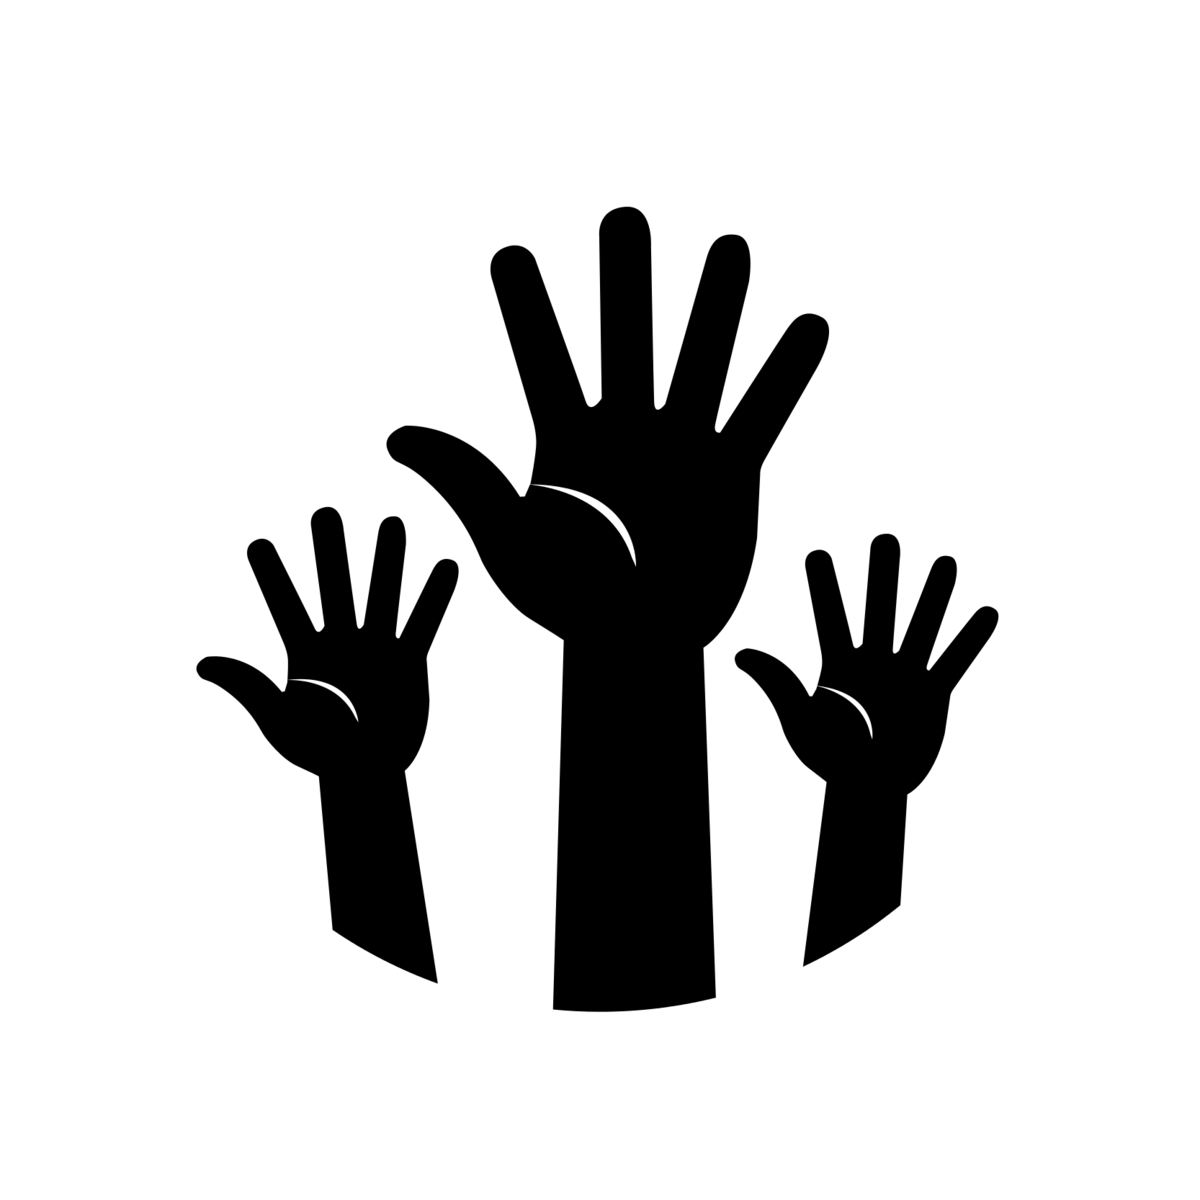
\includegraphics[scale=0.1]{images/hands.png}

\end{frame}
%----------------------------------------------------------------------
\begin{frame}[c]{}

\centering
\huge
Lecture 1:\\
Overview and Motivation
\end{frame}
%----------------------------------------------------------------------
%----------------------------------------------------------------------
\begin{frame}[c]{Overview}

What do we learn today?

\begin{itemize}
  \item Why ML does not scale up
  \item Design decisions in ML 
  \item What is AutoML? 
  \item Challenges in AutoML
  \item Risks of AutoML
  \item Meta-algorithmic hierarchy 
  \item Organization of the course
\end{itemize}

\end{frame}
%-----------------------------------------------------------------------
%----------------------------------------------------------------------
\begin{frame}[c]{Machine Learning}

\centering
\textit{``Machine learning is the science of getting computers to act\\
 without being explicitly programmed.''}

\hfill by Andrew Ng

\end{frame}
%-----------------------------------------------------------------------
%----------------------------------------------------------------------
\begin{frame}[c]{Machine Learning}

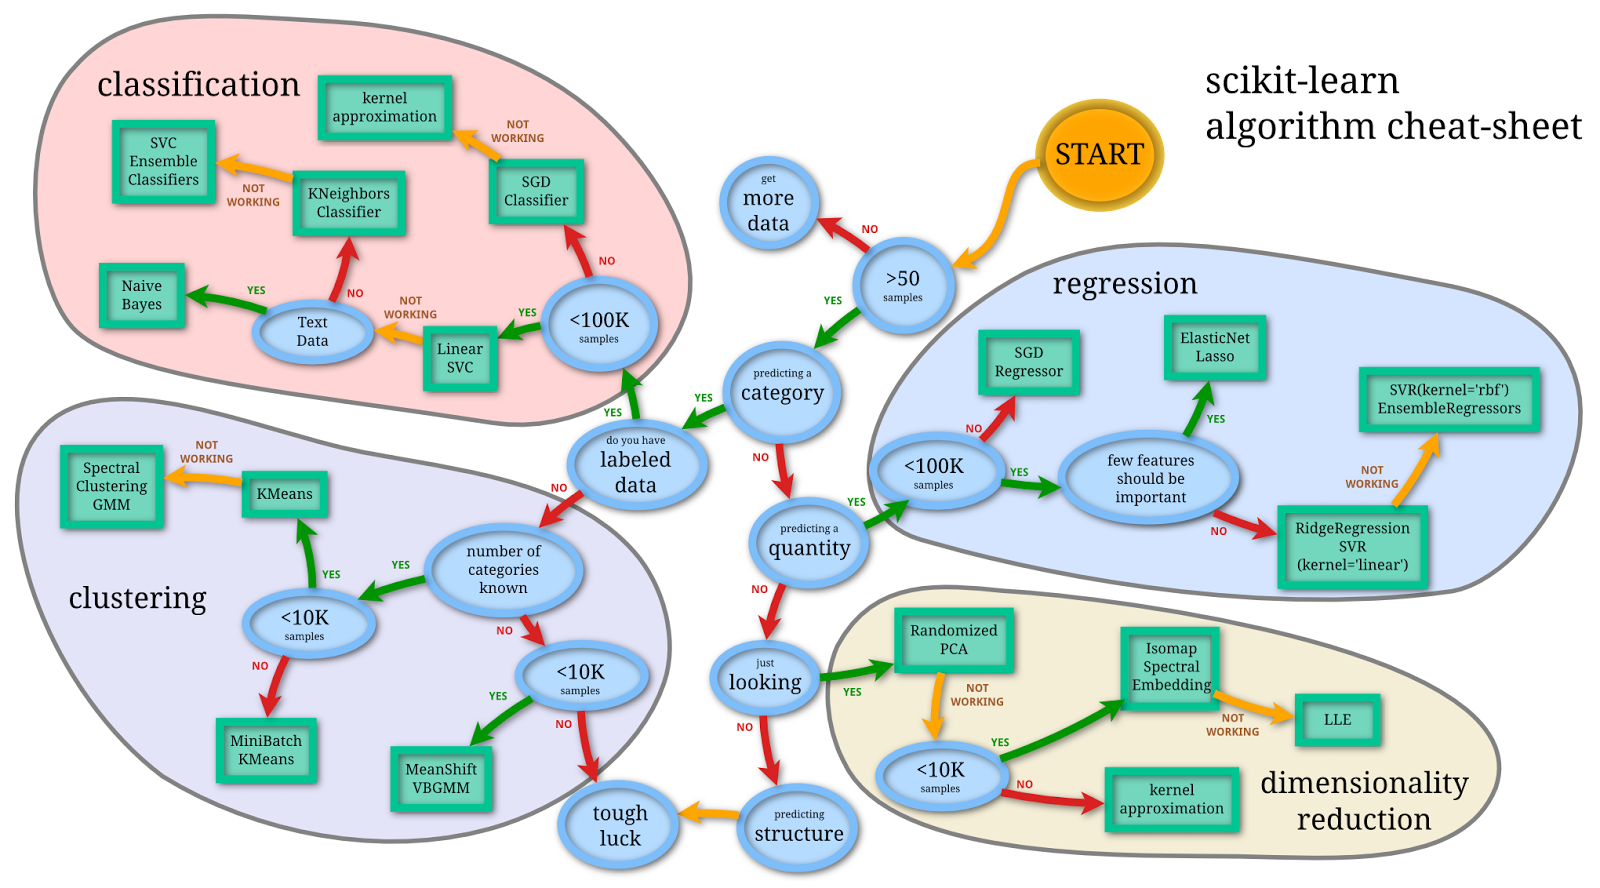
\includegraphics[width=1.0\textwidth]{images/sklearn-cheat}

\end{frame}
%-----------------------------------------------------------------------
%----------------------------------------------------------------------
\begin{frame}[c]{Machine Learning Workflow}

\centering
\tikzstyle{activity}=[rectangle, draw=black, rounded corners, text centered, text width=8em, fill=white, drop shadow]
\tikzstyle{wideactivity}=[rectangle, draw=black, rounded corners, text centered, text width=10em, fill=white, drop shadow]
\tikzstyle{data}=[rectangle, draw=black, text centered, fill=black!10, text width=8em, drop shadow]
\tikzstyle{myarrow}=[->, thick]
\begin{tikzpicture}[node distance=5cm,thick]
	\node (Train) [data] {DataSet $D_{\text{train}}$};
	\node (Fit) [activity, below of=Train, node distance=2cm] {Train model based on $D_{\text{train}}$};
	\draw[myarrow] (Train) -- (Fit);
	
	\pause
	
	\node (Test) [data, right of=Train] {DataSet $D_{\text{val}}$};
	\node (Eva) [activity, below of=Test, node distance=2cm] {Evaluate model on $D_{\text{val}}$};
	\draw[myarrow] (Fit) -- (Eva);
	\draw[myarrow] (Test) -- (Eva);
	
	\pause
	
	\node (user) [data, below of=Eva, node distance=2cm] {User};
	\draw[myarrow] (Eva) to node[right] {Performance} (user);
	
	\pause
	
	\node (Hyper) [activity, left of=user] {Adapt\\ Hyperparameters};
	\draw[myarrow] (user) to (Hyper);
	\draw[myarrow] (Hyper) to (Fit);
	
\end{tikzpicture}


\pause
 
\bigskip
\bigskip
$\leadsto$ Users indirectly teach machines how to learn.

\end{frame}
%-----------------------------------------------------------------------
%----------------------------------------------------------------------
\begin{frame}[c]{Machine Learning does not scale up}

\begin{itemize}
  \item Basics in machine learning are not hard to grasp
  \smallskip
  \item Achieving state-of-the-art performance is quite hard
  \smallskip
  \item Design decisions are (sometimes) unintuitive and\\ require a lot of expertise
  \begin{itemize}
    \item making these design decisions is a tedious and error-prone task
  \end{itemize}
  \smallskip
  \item Many experts are employed in ML these days
  \smallskip
  \item Nevertheless, developing a new ML-applications takes time
  \smallskip
  \item The job market for ML experts is nearly empty
\end{itemize}

\bigskip

\textit{``I'd like to use machine learning, but I can't invest much time''}

\hfill Zoubin Gharamani


\end{frame}
%-----------------------------------------------------------------------
%----------------------------------------------------------------------
\begin{frame}[c]{Design Decisions in Machine Learning}

What could be design decisions for applying ML to a new dataset?
\hands

\pause

\begin{itemize}
  \item Choice of machine learning algorithm
  \begin{itemize}
    \item SVM, random forest, deep neural network?
  \end{itemize}
  \pause
  \item Hyperparameters of machine learning algorithms
  \begin{itemize}
    \item SVM: C, gamma, kernel, \ldots?
  \end{itemize}
  \pause
  \item Architecture of a neural network
  \begin{itemize}
    \item $\#$layers, $\#$neurons, activation function, \ldots 
  \end{itemize}
  \pause
  \item Data preprocessing
  \begin{itemize}
  	\item data cleanup, missing data imputation, feature selection, \ldots  
  \end{itemize}
  \pause
  \item anomaly detection
  \item allocation of computational resources
  \item \ldots
\end{itemize}

\medskip
$\leadsto$ All these design decisions have to be made for each new dataset.

\end{frame}
%-----------------------------------------------------------------------
%----------------------------------------------------------------------
\begin{frame}[c]{A simple Example with $k$-NN}

\centering
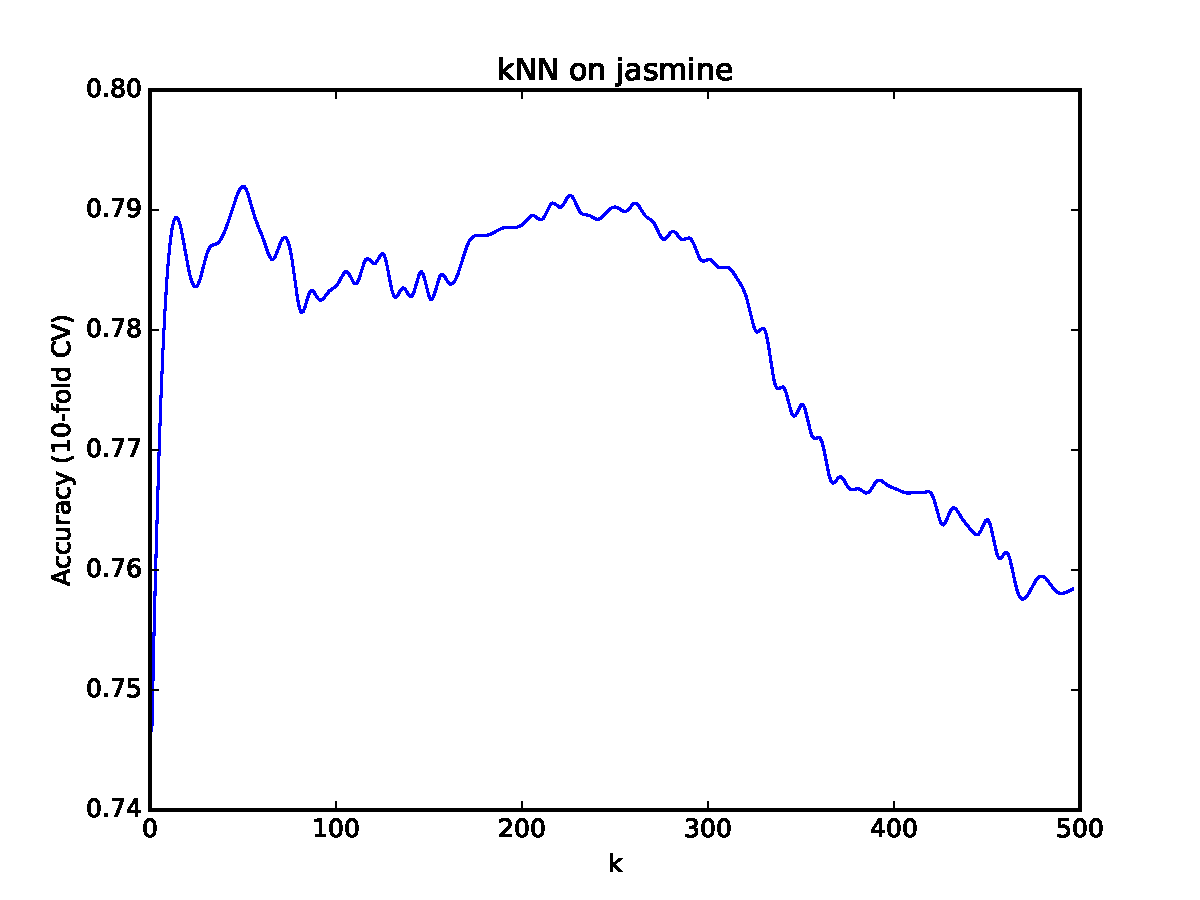
\includegraphics[width=0.6\textwidth]{images/kNN-jasmine}

\begin{itemize}
  \item $k$-nearest neighbors is one of the most trivial ML algorithms
  \item Size of neighbourhood ($k$) is very important for its performance
  \item The performance function depending on $k$ is quite complex\\ (not at all convex)
\end{itemize}

\end{frame}
%-----------------------------------------------------------------------
%----------------------------------------------------------------------
\begin{frame}[c]{Goal of AutoML}

\begin{block}{AutoML}
The goal of AutoML is to automate all parts of machine learning (as needed)
to \emph{support} users efficiently building their machine learning applications.
\end{block}

\bigskip

\begin{block}{AutoML System}
Given
\begin{itemize}
  \item a dataset
  \item a task (e.g., regression or classification)
  \item a performance metric (e.g., accuracy or RMSE)
\end{itemize}
an AutoML system automatically determines the approach 
that performs best for this particular application.
\end{block}

\end{frame}
%-----------------------------------------------------------------------
%----------------------------------------------------------------------
\begin{frame}[c]{AutoML in Research}

AutoML enables:

\begin{enumerate}
  \item more efficient research
  \begin{itemize}
    \item AutoML has shown on subproblems to outperform human experts
  \end{itemize}
  \pause
  \smallskip
  \item more systematic research
  \begin{itemize}
    \item humans tend to be unsystematic which leads to errors
  \end{itemize}
  \smallskip
  \pause
  \item more reproducible research
  \begin{itemize}
    \item since AutoML is systematic and human's unsystematic approaches cannot be reproduced 
  \end{itemize}
  \item broader use of ML also in other disciplines
  \begin{itemize}
    \item ML should not be limited to computer scientists;
    \item the most amazing applications of ML is often done\\ by either interdisciplinary teams or even non-computer scientists
  \end{itemize}
\end{enumerate}

\end{frame}
%-----------------------------------------------------------------------
%----------------------------------------------------------------------
\begin{frame}[c]{Challenges in AutoML}

\begin{enumerate}
  \item Design decisions have to be made for each dataset again
  \item Training of a single ML model can be quite expensive\\
  		(e.g., hours, days or weeks)
  \begin{itemize}
    \item[$\leadsto$] often, we cannot try a many design decisions
  \end{itemize}
  \item the mathmatical relation between design decisions\\ and performance is (often) unknown
  \begin{itemize}
    \item[$\leadsto$] gradient-based optimization is not directly possible
  \end{itemize}
  \item optimization in highly complex spaces
  \begin{itemize}
    \item incl. categorical choices, continuous parameters,\\ conditional dependencies
  \end{itemize}
  
\end{enumerate}

\end{frame}
%-----------------------------------------------------------------------
%----------------------------------------------------------------------
\begin{frame}[c]{Risks of AutoML}

What could be risks of AutoML?
\hands
\pause

\begin{enumerate}
  \item Users apply AutoML without understanding anything.
  \begin{itemize}
    \item Users might wonder why (Auto-)ML does not perform well\\ after they passed poor data. 
  \end{itemize}
  \pause
  \item The users over-trust the AutoML too much.
  \begin{itemize}
    \item humans might not use human reasoning skills and do not second guess machine decisions
  \end{itemize}
  \pause
  \item We enable non-ML experts to use ML\\ without knowing the risks and consequences of ML.
  \pause
  \item Could result in deployment of \ldots
  \begin{itemize}
    \item inaccurate ML models due to lack of understanding of statistical concepts, e.g., sampling bias, overfitting, concept drift, \ldots
    \item biased and unfair models due to lack of understanding ethical practices and use of features such as gender and race for predicting outcomes
  \end{itemize}
\end{enumerate}

See \textit{\href{https://arxiv.org/abs/1902.06804}{Democratisation of Usable Machine Learning in Computer Vision}}

\end{frame}
%-----------------------------------------------------------------------
%----------------------------------------------------------------------
\begin{frame}[c]{Snipped of Meta-Algorithmic Hierarchy}


Meta-algorithmic approaches

\begin{itemize}
  \item[$\subset$] AutoAI
  \pause
  \begin{itemize}
		\item[$\subset$] AutoML
		\pause
		\begin{itemize}
		 	\item[$\subset$] Hyperparameter optimization (HPO)
		 	\pause
		 	\item[$\subset$] Neural architecture search (NAS)\\
		 	   \hspace{1em} Google sometimes claims: AutoML $==$ NAS\\
		 	   \hspace{1em} but that's wrong!
		 	\pause
		 	\item[$\subset$] Meta-learning\\
		\end{itemize}
		\pause
		\item[$\subset$] Algorithm configuration
	\end{itemize}
	\pause
	\item[$\subset$] Search-based software engineering
\end{itemize}

\end{frame}
%-----------------------------------------------------------------------
%----------------------------------------------------------------------
\begin{frame}[c]{Goals of the Lecture}

You will be able to \ldots
\begin{enumerate}
  \item use AutoML tools
  \smallskip
  \item develop AutoML tools
  \smallskip
  \item have a good overview over the state-of-the-art in AutoML
  \smallskip
  \item do research on AutoML yourself
  \begin{itemize}
    \item perfect opportunity to do a master project or thesis with us afterwards
  \end{itemize}
\end{enumerate}

\end{frame}
%-----------------------------------------------------------------------
%----------------------------------------------------------------------
\begin{frame}[c]{Course Overview}

\begin{itemize}
	\item Introduction
	\item Background
	\begin{itemize}
		\item Design spaces in ML
		\item Experimentation and visualization
	\end{itemize}
	\item Hyperparameter optimization (HPO)
	\begin{itemize}
	  \item Bayesian optimization
	  \item Other black-box techniques
	\end{itemize}
	\item Speeding up HPO with multi-fidelity optimization
	\item Pentecost (Holiday) -- no lecture
	\item Architecture search I + II
	\item Meta-Learning
	\item Learning to learn $\&$ optimize
	\item Beyond AutoML: algorithm configuration and control
	\item Project announcement and closing
\end{itemize}


\end{frame}
%----------------------------------------------------------------------
%----------------------------------------------------------------------
\begin{frame}[c]{Course Format}

\begin{itemize}
	\item Concepts over details
	\begin{itemize}
	  \item we provide references and links to papers\\ s.t. you can read up details!
	\end{itemize}
	\smallskip
	\item Interactive lecture
	\begin{itemize}
	  \item more efficient learning through self-reflection on challenges!
	\end{itemize}
	\smallskip
	\item Practical exercises
	\begin{itemize}
	  \item implement it, use it and play with it!
	\end{itemize}
\end{itemize}

\end{frame}
%----------------------------------------------------------------------
%----------------------------------------------------------------------
\begin{frame}[c]{Team - Lectures}

\begin{columns}[T]
\column{0.3\textwidth}

\centering
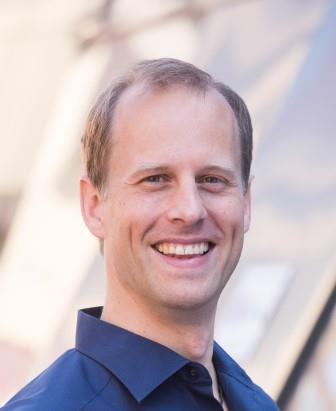
\includegraphics[width=9em]{images/team/frank_small}

Prof. Dr. Frank Hutter

\column{0.3\textwidth}
\centering
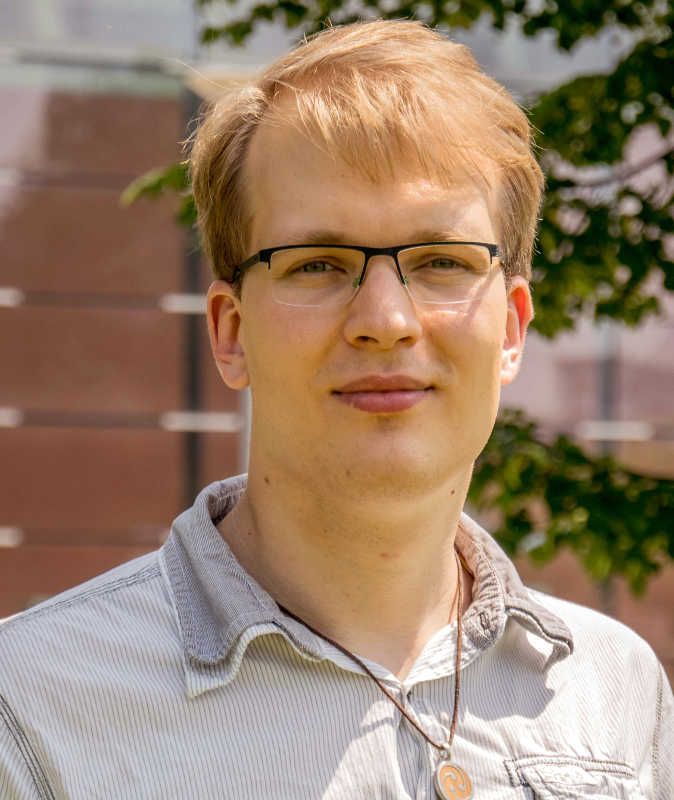
\includegraphics[width=9em]{images/team/marius}

Dr. Marius Lindauer

\column{0.3\textwidth}
\centering
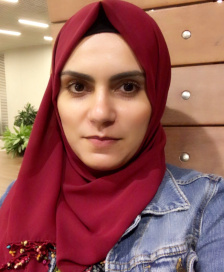
\includegraphics[width=9em]{images/team/awad_small}

Dr. Noor Awad\\
(guest lecturer)


\end{columns}

\end{frame}
%----------------------------------------------------------------------
%----------------------------------------------------------------------
\begin{frame}[c]{Team -- Exercise}

\begin{columns}[T]

\column{0.3\textwidth}
\centering
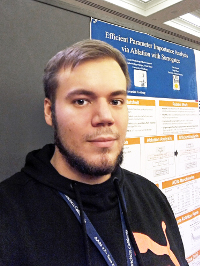
\includegraphics[height=9em]{images/team/biedenkapp}
André Biedenkapp
\column{0.3\textwidth}
\centering
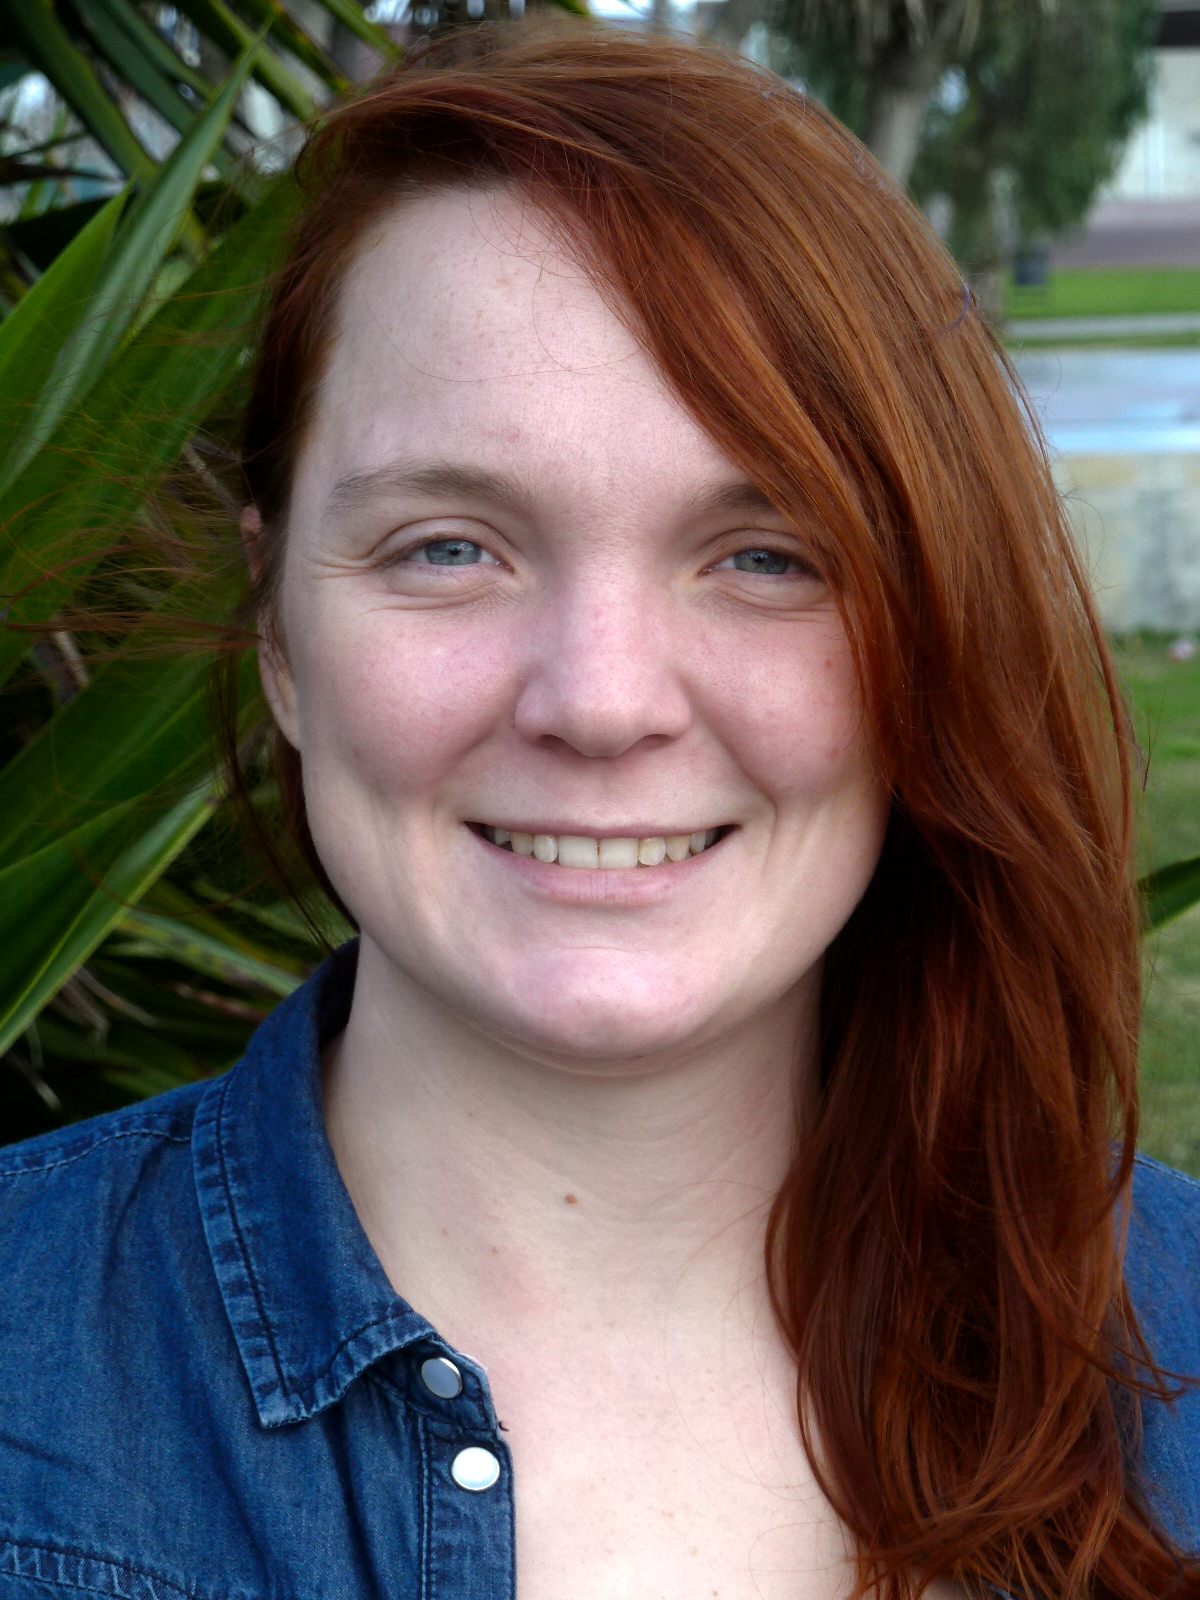
\includegraphics[height=9em]{images/team/eggensperger_small}
Katharina Eggensperger
\column{0.3\textwidth}
\centering
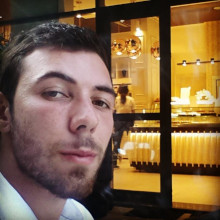
\includegraphics[height=9em]{images/team/arber_small}
Arber Zela

\end{columns}

\end{frame}
%----------------------------------------------------------------------
%----------------------------------------------------------------------
\begin{frame}[c]{Organization (Lectures)}

\begin{itemize}
  \item $6$ ECTS
  \item Every week at Monday: 14:15 (s.t) - 15:45\\ (Building: 106 Room: SR 00 007)
  \item \emph{Interactive} Lecture 
  \begin{itemize}
    \item We will ask you questions in the lectures
    \item Kahoot quiz at the end of each lecture
  \end{itemize}
  \item Course material on our homepage\\
  		{\small \url{ml.informatik.uni-freiburg.de/teaching/ss2019/automl/}}
  \item Slides will be online before the lectures
  \item No video recording!
\end{itemize}

\end{frame}
%-----------------------------------------------------------------------
%----------------------------------------------------------------------
\begin{frame}[c]{Organization (Exercises)}

\begin{itemize}
  \item Every Friday at: 14:15 - 15:45\\ (Building: 106 Room: SR 00 007)
  \begin{itemize}
    \item No meeting this week, but first exercise sheet!
  \end{itemize}
  \item Every week new exercise sheet and discussion of last exercise
  \item Most exercises will be practical, i.e., you have to implement something
  \item Team work allowed, max team size: 2! 
  \item Cheating:
  \begin{itemize}
    \item First time cheating: $0$ points for exercise
    \item Second time cheating: failing the course
  \end{itemize}
  \item You have to obtain at least $50\%$ points in the exercises  
  \item The number of points per sheet will slightly increase over time
  \item Submit via bitbucket (git)
\end{itemize}

\end{frame}
%-----------------------------------------------------------------------
%----------------------------------------------------------------------
% \begin{frame}[c]{Exceptions (tentative)}
% 
% \begin{itemize}
% 	\item No lectures and exercises during vacations and holidays\\ (1. Nov, 25. Dec, 27. Dec, 01. Jan, 03. Jan)
% 	\item Switching lecture and exercise slot 11. Dec and 13. Dec
% 	\item Last lecture at 05. Feb
% \end{itemize}
% 
% \end{frame}
%-----------------------------------------------------------------------
%----------------------------------------------------------------------
\begin{frame}[c]{Requirements}

\begin{itemize}
  \item Knowledge in \alert{Machine Learning} (strongly recommended)
  \begin{itemize}
    \item Classification, regression, clustering, decision tree, training-test split, cross validation, pre-processing \ldots
  \end{itemize}
  \pause
  \item Knowledge in \alert{Deep Learning} (strongly recommended)
  \begin{itemize}
    \item feed-forward network, recurrent network, convolutions, learning rates, regularization, \ldots 
  \end{itemize}
  \pause
  \item Experience in \alert{Python and git} (recommended)
  \begin{itemize}
    \item nearly all exercises will require 
    that you implement something in~Python and submit the solution to a git repo
  \end{itemize}
\end{itemize}

\end{frame}
%-----------------------------------------------------------------------
%----------------------------------------------------------------------
\begin{frame}[c]{Final Oral Exam}

\begin{itemize}
  \item Implement a larger project (worth $1-2$ weeks fulltime)
	\begin{itemize}
		\item No teamwork!
	\end{itemize}
  \item Exam
	\begin{itemize}
		\item Present the project in the first $15$ minutes\\ (including some questions from us)
		\item Answer questions about further course material in the second $15$ minutes
	\end{itemize}	
  \item tentative date: end of September
\end{itemize}

\end{frame}
%----------------------------------------------------------------------
%----------------------------------------------------------------------
\begin{frame}[c]{Resources}

\begin{itemize}
  \item To get a deep understanding of AutoML, you should also read some literature 
  \item We will provide links to papers at the end of each lecture
  \item New AutoML book: \url{https://www.automl.org/book/}
  \begin{itemize}
    \item Draft online available
  \end{itemize}
\end{itemize}

\end{frame}
%----------------------------------------------------------------------
%----------------------------------------------------------------------
\begin{frame}[c]{Chances and Risks}

AutoML is an advanced lecture and we modify it each time.

\bigskip
\pause

Chances:
\begin{itemize}
  \item All presented topics are close to state-of-the-art;\\there is active research on these topics  
  \item The course will provide a solid background\\ for doing a master project/thesis in our group 
\end{itemize}

\medskip

Risks:
\begin{itemize}
  \item You will find some typos and issues in the slides;\\ please tell us if you find something
  %\item Workload could be very high for you -- we have no experience with the exercises yet
\end{itemize}

\medskip
\pause
$\to$ Give us some feedback and we will improve the course!

\medskip
\pause
Note: AutoML was already partially covered in our old lecture ML4AAD. 
If you successfully attended ML4AAD, please don't attend AutoML.

\end{frame}
%-----------------------------------------------------------------------
%----------------------------------------------------------------------
\begin{frame}[c]{Introduce yourself!}

\begin{itemize}
  \item Why have you chosen this course?
  \medskip
  \item Background knowledge? (ML, DL, \ldots)
  \medskip 
  \item Experience with such problems?
\end{itemize}

\bigskip
\centering
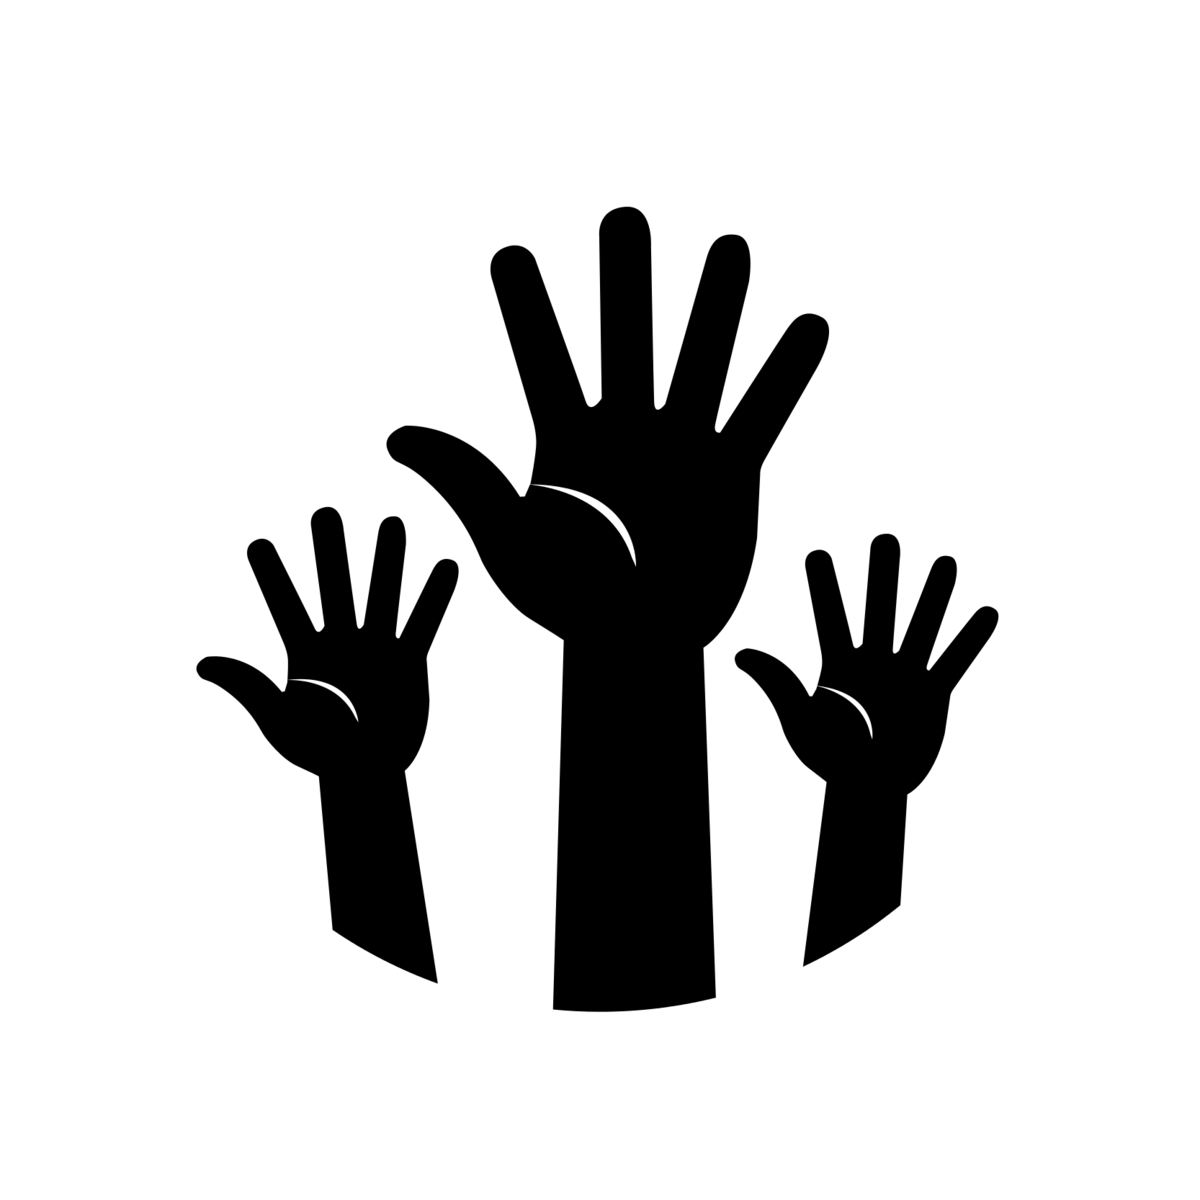
\includegraphics[scale=0.1]{images/hands.png}

\end{frame}
%-----------------------------------------------------------------------
%----------------------------------------------------------------------
% \begin{frame}[c]{Exercise I }
% 
% \begin{block}{Task}
% \begin{enumerate}
% 	\item Identify $2$ (known) algorithms which have tunable parameters and briefly describe these parameters
% 	\item Describe a manual way to tune the parameters and approximate the effort you would need to do this on an example
% 	\item Analyze the runtime complexity of the algorithms
% \end{enumerate}
% \end{block}
% 
% \alert{Submission due 02.11. (23:59 GMT)}\\
% Submit at ILIAS : \url{https://ilias.uni-freiburg.de/goto.php?target=crs_465155&client_id=unifreiburg}
% %Send to: \url{lindauer@cs.uni-freiburg.de}\\
% %with subject: \texttt{[MLOAD Excercise I] $<$your name$>$} 
% 
% \end{frame}
%-----------------------------------------------------------------------
% %----------------------------------------------------------------------
% \begin{frame}[c]{}
% 
% 
% 
% \end{frame}
% %-----------------------------------------------------------------------


%%----------------------------------------------------------------------
\begin{frame}[c]{Where are we? The big picture}

\begin{itemize}
\item[$\to$] Algorithm Selection
  \begin{itemize}
    \item[$\to$] Portfolios
    \item Algorithm selection for runtime
  \end{itemize}
  \item Design Decisions:\\ Local Search + Evo. Algorithms + Machine Learning 
  \item Empirical evaluation
  \item AAD for ML
  \begin{itemize}
    \item Hyperparameter optimization and Bayesian Optimization 
    \item Neural architecture search (lecture given by Prof. Hutter)
  \end{itemize}
  \item Algorithm configuration 
  \begin{itemize}
    \item Basics 
    \item State of the art 
    \item Best Practices 
  \end{itemize}
  \item Combinations of algorithm selection and configurations
  \item Algorithm control 
  \item Algorithm analysis 
  \item Project announcment and questions for exam
\end{itemize}

\end{frame}
%----------------------------------------------------------------------
%----------------------------------------------------------------------
\begin{frame}[c]{}

\centering
\huge
Algorithm Portfolios and\\ Algorithm Selection

\bigskip
\includegraphics[width=0.8\textwidth]{images/algorithm_selection}

\end{frame}
%----------------------------------------------------------------------
%----------------------------------------------------------------------
\begin{frame}[c]{Motivation: Complementarity of Algorithms}

Real-world example (see SAT12-ALL scenario of ASlib):

\begin{itemize}
  \item Algorithm A (``sparrow'') on Instance X took $1.76$ sec
  \item Algorithm B (``glucose2'') on Instance X had a timeout ($\geq 1200$ sec)
  \pause
  \medskip
  \item Algorithm A (``sparrow'') on Instance Y had a timeout ($\geq 1200$ sec)
  \item Algorithm B (``glucose2'') on Instance Y took $24.1$ sec
\end{itemize}

\pause
$\leadsto$ Algorithms have different strengthes and weaknesses!

\pause
\bigskip
\begin{block}{Complementarity of Algorithms}
Two algorithms are complementary if they perform well on different kinds of instances.
\end{block}

\pause
(Definition of complementarity can be extended to sets of algorithms.)


\end{frame}
%-----------------------------------------------------------------------
%----------------------------------------------------------------------
\begin{frame}[c]{Learning Goals}

After this lecture, you will be able to \ldots

\begin{itemize}
  \item \alert{exploit complementarity} of algorithms to improve overall performance
  \item explain \alert{algorithm portfolios} and its different variants
  \begin{itemize}
    \item racing portfolios
    \item parallel portfolios
    \item algorithm schedules
  \end{itemize}
  \item define \alert{per-instance algorithm selection} and to describe one specific implementation 
  \item explain different types of \alert{instance features}
\end{itemize}

\end{frame}
%----------------------------------------------------------------------
%----------------------------------------------------------------------
\begin{frame}[c]{Prerequisite: Instances}

\begin{block}{What are instances?}
``Instances'' are inputs to an algorithm and the algorithm has to process instances.
In the end, the algorithm will return an output to an instance (a.k.a. the instance was ``solved'').
\end{block}

\pause

Synonyms:
\begin{itemize}
  \item Algorithm input
  \item Task
\end{itemize}

\pause

Examples:
\begin{itemize}
  \item Dataset for a machine learning algorithm
  \item Planning problem for an AI planning solver
  \item Mixed-integer program for a MIP solver
  \item CNF instance for a SAT solver
  \item Datatable for a database
\end{itemize}

\end{frame}
%----------------------------------------------------------------------
%----------------------------------------------------------------------
\begin{frame}[c]{Setting (today and next week)}

\includegraphics[width=0.9\textwidth]{images/as_setting}

\end{frame}
%----------------------------------------------------------------------

%----------------------------------------------------------------------
\begin{frame}[c]{Example: SAT Challenge 2012}

\centering
\includegraphics[scale=0.3]{images/satchallenge12_indu.png}

\begin{description}
  \item[green] A single algorithm on each instance
  \item[blue] A fixed set of algorithms solving each instance ``together''
  \item[pink] Algorithm selection approaches: Select the best algorithm for the instance at hand 
\end{description}

\end{frame}
%----------------------------------------------------------------------
%----------------------------------------------------------------------
\begin{frame}[c]{Oracle / Virtual Best Solver (VBS)}

\begin{block}{Intuition}
Given a portfolio (set) of algorithms, the oracle is the portfolio system
that always selects the best component algorithm for a given instance.
\end{block}

\pause
\bigskip

\begin{block}{Definition}
Given 
\begin{itemize}
  \item a portfolio (set) of algorithms $\portfolio$,
  \item a set of instances $\insts$,
  \item a cost metric $c: \portfolio \times \insts \to \perf$, 
\end{itemize} 
the cost of the oracle is $\sum_{\inst \in \insts} \min_{\algo \in \portfolio} c(\algo, \inst)$.
\end{block}

%Note: We do not consider information sharing between the algorithms in this setting.

\end{frame}
%-----------------------------------------------------------------------
%----------------------------------------------------------------------
\begin{frame}[c]{Toy Example: Oracle}

\[
\begin{array}{| r | c  c  c || c |}
  \cline{1-5}
      & \algo_1 & \algo_2 & \algo_3 & oracle\\
  \cline{1-5}
  \inst_1 & 		 1    &         10  &         3    & 1 \\
  \inst_2 &          5    &         10  &  		2 	  & 2 \\
  \inst_3 &          8    &  		1    &         10  & 1 \\
  \inst_4 &         10  &         10  & 		2 	  & 2 \\
  \inst_5 &         10  & 		 6    &         10  & 6 \\
  \inst_6 &         10  &          8    &         10  & 8 \\
  \cline{1-5}
  \onslide<2->{\varnothing & 7.3 & 7.5 & 6.1 & 3.3}\\
  %\text{timeouts} & 3 & 3 & 3 & 0 \\ 
  \cline{1-5}
\end{array}
\]


\end{frame}
%-----------------------------------------------------------------------
%----------------------------------------------------------------------
\begin{frame}[c]{Baseline: Single Best (SB)}

\begin{block}{Intuition}
If we don't use a portfolio, we would simply pick the best single algorithm.
\end{block}

\pause
\bigskip

\begin{block}{Definition}
Given a portfolio (set) of algorithms $\portfolio$, a set of instances $\insts$,
a cost metric $c: \portfolio \times \insts \to \perf$,
the single best (SB) algorithm is $\argmin_{\algo \in \portfolio} \sum_{\inst \in \insts} c(\algo, \inst)$
\end{block}

\pause
\bigskip

$\leadsto$ A portfolio system should have a performance\\ between the SB's performance and the oracle's performance.

\end{frame}
%-----------------------------------------------------------------------
%----------------------------------------------------------------------
\begin{frame}[c]{Toy Example: SB}

\[
\begin{array}{| r | c  c  c || c |}
  \cline{1-5}
      & \algo_1 & \algo_2 & \algo_3 & oracle\\
  \cline{1-5}
  \inst_1 & 		 1    &         10  &         3    & 1 \\
  \inst_2 &          5    &         10  &  		2 	  & 2 \\
  \inst_3 &          8    &  		1    &         10  & 1 \\
  \inst_4 &         10  &         10  & 		2 	  & 2 \\
  \inst_5 &         10  & 		 6    &         10  & 6 \\
  \inst_6 &         10  &          8    &         10  & 8 \\
  \cline{1-5}
  \varnothing & 7.3 & 7.5 & 6.1 & 3.3\\
  %\text{timeouts} & 3 & 3 & 3 & 0 \\ 
  \cline{1-5}
\end{array}
\]

\bigskip

$\to$ $\algo_3$ is the single best algorithm

\end{frame}
%-----------------------------------------------------------------------
\begin{frame}[c]{Oracle and SB in Practice}

\begin{tabular}{lrr}
\toprule
Domain 										& Oracle 	& Single Best \\
\midrule
Structure learning in Bayesian networks 	& $219.86$ 	& $9017.07$\\
Constraint Satisfaction Problem (CSP)		& $26.27$	& $1605.36$ \\
Maximum Satisfiability Problem (MAXSAT) 	& $101.34$	& $1572.00$\\
Mixed Integer Programming (MIP)				& $281.51$	& $3007.92$\\
Quantified Boolean Formula (QBF)			& $9.99$	& $2642.89$	\\
Boolean Satisfiability Problem 	(SAT12-ALL)	& $97.84$	& $2962.29$\\
\midrule
Machine Learning (OPENML-Weka; Error)		& $12.5\%$	& $14.5\%$\\
\bottomrule
\end{tabular}

\lit{Source: Open Algorithm Selection Challenge 2017}

\end{frame}
%----------------------------------------------------------------------
\begin{frame}[c]{Parallel algorithm portfolios~\litw{B. Huberman et al. 1997}}

\begin{block}{Definition}
Given a portfolio (set) of algorithms $\portfolio$ of size $k$ and $k$ parallel computation units (e.g., CPU cores),
a parallel portfolio system runs each $\algo \in \portfolio$ on one parallel computation unit in parallel.
The first $\algo$ that ``solved'' the instance at hand, terminates all other algorithms.  
\end{block}

\pause
$\leadsto$ Cost metric $c$ should relate to runtime of an algorithm. 


\bigskip
\pause

\begin{block}{Performance}
For a given set of instances $\insts$ and
a cost metric $c: \portfolio \times \insts \to \perf$,
the cost of a parallel algorithm portfolio is $\sum_{\inst \in \insts} \min_{\algo \in \portfolio} c(\algo, \inst) + \epsilon_{k}$
where $\epsilon_{k}$ is overhead induced by using $k$ parallel computation units in parallel.
\end{block}

\end{frame}
%-----------------------------------------------------------------------
%----------------------------------------------------------------------
\begin{frame}[c]{Parallel portfolios for SAT~\litw{Lindauer et al. 2017}}

\small
%\onslide<1->{PAR$X$ is the penalized average runtime where each timeout is counted as $X$ times the runtime cutoff.}

\begin{center}
\begin{tabular}{lrrrr}
\toprule
$\#$ Units   & \multicolumn{2}{c}{\lingeling} & \multicolumn{2}{c}{\clasp} \\
	 & \multicolumn{2}{c}{Industrial} & \multicolumn{2}{c}{Crafted}  \\
\midrule
& $\#$Timeouts & $\varnothing_t$ & $\#$Timeouts & $\varnothing_t$\\
\cmidrule{2-3}\cmidrule{4-5}
$1$ & $82$ & $380$ & $136$ & $464$\\
\pause
$2$ & $65$ & $331$ & $118$ & $421$\\
\pause
$3$ & $60$ & $313$ & $115$ & $410$\\
\pause
$4$ & $56$ & $308$ & $115$ & $402$\\
$5$ & $58$ & $312$ & $105$ & $384$\\
$6$ & $60$ & $315$ & $103$ & $380$\\
$7$ & $59$ & $309$ & $102$ & $372$\\
$8$ & $55$ & $303$ & $96$ & $353$\\
\bottomrule
\end{tabular}
\end{center}

\end{frame}
%-----------------------------------------------------------------------
%----------------------------------------------------------------------
\begin{frame}[c]{Overhead $\epsilon_k$}

\small
We ran the \alert{same} (deterministic) configuration of \lingeling{} (\clasp{}, resp.) $k$ times in parallel.

\begin{center}
\begin{tabular}{crrrrrr}
\toprule
$\#$ Units   & \multicolumn{2}{c}{\lingeling} & \multicolumn{2}{c}{\clasp} \\
Set & \multicolumn{2}{c}{Industrial} & \multicolumn{2}{c}{Crafted}  \\
\midrule
& $\#$Timeouts & $\varnothing_t$ & $\#$Timeouts & $\varnothing_t$\\
\cmidrule{2-3}\cmidrule{4-5}
$1$ & $82$ & $380$ & $136$ & $464$\\
\pause
$2$ & $79$ & $376$ & $134$ & $461$\\
\pause
$3$ & $85$ & $376$ & $135$ & $451$\\
\pause
$4$ & $86$ & $382$ & $135$ & $452$\\
$5$ & $89$ & $385$ & $135$ & $463$\\
$6$ & $90$ & $390$ & $135$ & $465$\\
$7$ & $90$ & $390$ & $135$ & $465$\\
$8$ & $92$ & $393$ & $136$ & $467$\\
\bottomrule
\end{tabular}
\end{center}
 
 $\leadsto$ Most algorithms developed for runtime are sensitive to cache misses.
 
\end{frame}
%-----------------------------------------------------------------------
%----------------------------------------------------------------------
\begin{frame}[c]{Sequential portfolios~\litw{B. Huberman et al. 1997, Gomes and Selman 2001}}

\begin{block}{Definition}
Given a portfolio (set) of algorithms $\portfolio$ of size $k$,
a sequential portfolio system runs all $\algo \in \portfolio$ on \alert{the same computation unit} in ``parallel'' (e.g., round robin).
The first $\algo$ that ``solved'' the instance at hand, terminates all other algorithms.  
\end{block}

\bigskip
\pause

\begin{itemize}
  \item each algorithm has only $\frac{1}{k}$ of the overall available time budget (cutoff) and memory
  \item (In practice, the operating system (OS) will use a round-robin schedule)
\end{itemize}

\end{frame}
%-----------------------------------------------------------------------
%----------------------------------------------------------------------
\begin{frame}[c]{Toy Example: Sequential portfolio}

\begin{itemize}
  \item Runtime cutoff $\kappa = 10$
  \item performance metric $m$: runtime
\end{itemize}

%\medskip

\[
\begin{array}{| r | c  c  c || c | c |}
  \cline{1-6}
      & \algo_1 & \algo_2 & \algo_3 & oracle & Seq. \portfolio\\
  \cline{1-6}
  \inst_1 & 		 1    &         10  &         3    & 1  & ?\\
  \inst_2 &          5    &         10  &  		2 	  & 2 & ?\\
  \inst_3 &          8    &  		1    &         10  & 1 & ?\\
  \inst_4 &         10  &         10  & 		2 	  & 2 & ?\\
  \inst_5 &         10  & 		 6    &         10  & 6 & ?\\
  \inst_6 &         10  &          8    &         10  & 8 & ?\\
  \cline{1-6}
\end{array}
\]

\centering
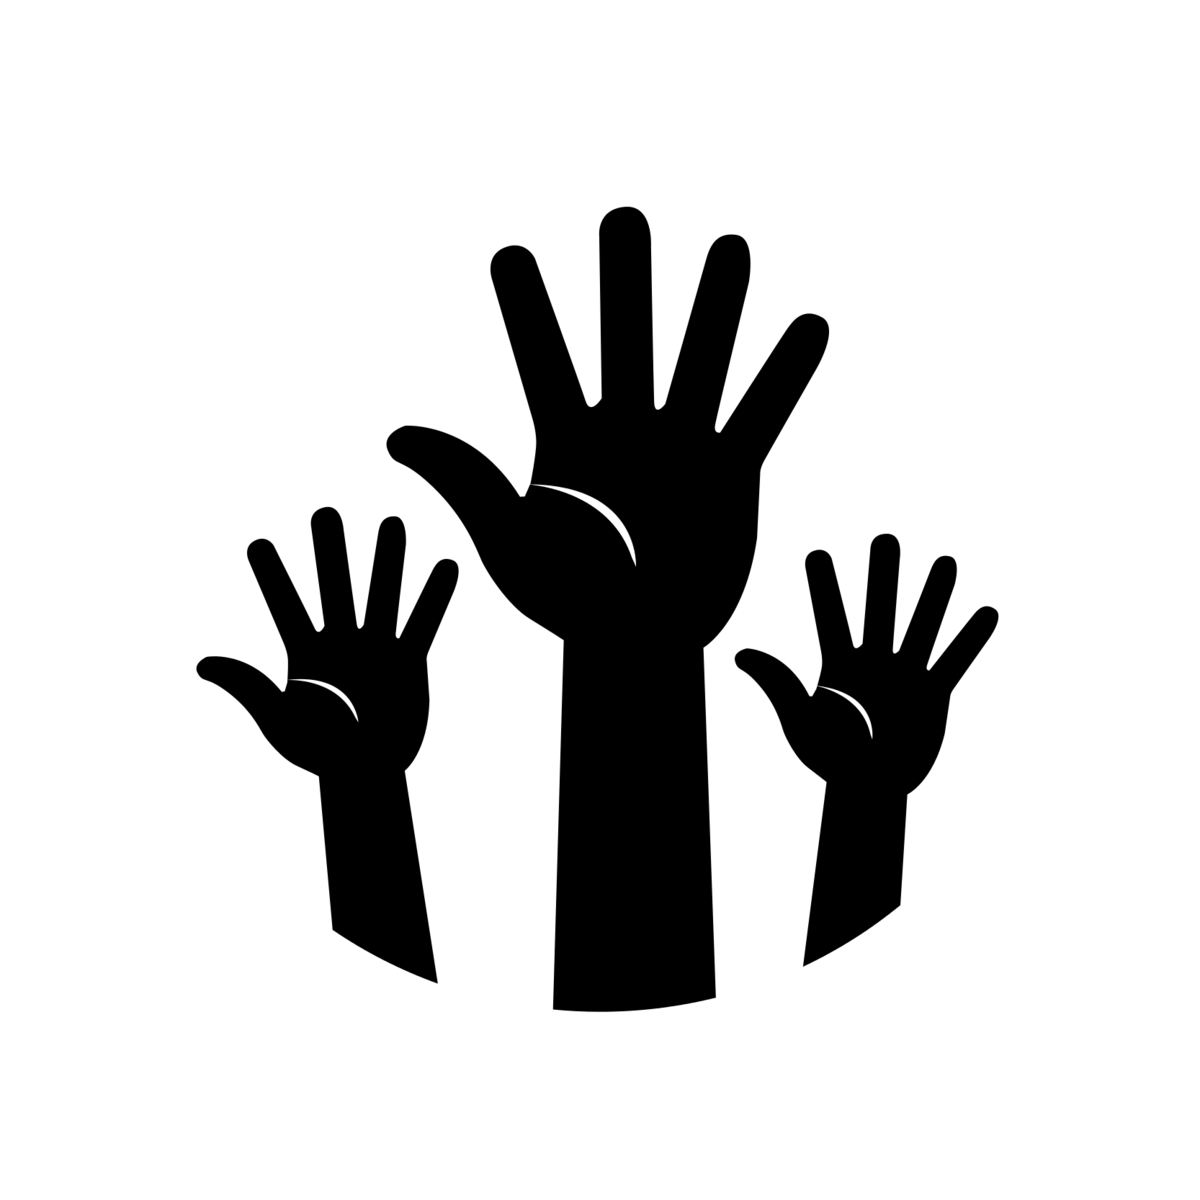
\includegraphics[height=1cm]{images/hands.png}

\end{frame}
%-----------------------------------------------------------------------
%----------------------------------------------------------------------
\begin{frame}[c]{Toy Example: Sequential portfolio}

\begin{itemize}
  \item Runtime cutoff $\kappa = 10$
  \item performance metric $m$: average runtime \onslide<3->{or timeouts}
\end{itemize}

%\medskip

\[
\begin{array}{| r | c  c  c || c | c |}
  \cline{1-6}
      & \algo_1 & \algo_2 & \algo_3 & oracle & Seq. \portfolio\\
  \cline{1-6}
  \inst_1 & 		 1    &         10  &         3    & 1  & 3\\
  \inst_2 &          5    &         10  &  		2 	  & 2 & 6\\
  \inst_3 &          8    &  		1    &         10  & 1 & 3\\
  \inst_4 &         10  &         10  & 		2 	  & 2 & 6\\
  \inst_5 &         10  & 		 6    &         10  & 6 & 10\\
  \inst_6 &         10  &          8    &         10  & 8 & 10\\
  \cline{1-6}
  \onslide<2->{\varnothing & 7.3 & 7.5 & 6.1 & 3.3 & 6.3}\\
  \cline{1-6}
  \onslide<3->{\text{timeouts} & 3 & 3 & 3 & 0 & 2}\\ 
  \cline{1-6}
\end{array}
\]

\onslide<4->{\textit{ppfolio} won many gold medals at the SAT Competition 2011\\ with such a simple approach.}


\end{frame}
%-----------------------------------------------------------------------
%----------------------------------------------------------------------
\begin{frame}[c]{Algorithm Schedules}

\begin{block}{Idea}
Instead of running a uniform schedule with pseudo parallelism (a.k.a. seq. portfolio),
run a non-uniform, ordered schedule of algorithms.
\end{block}

\pause
\begin{itemize}
  \item Runtime cutoff $\kappa = 10$
  \item Schedule: $[\algo_1 \mapsto 1, \algo_3 \mapsto 2, \algo_2 \mapsto 7]$
\end{itemize}

\pause
\[
\begin{array}{| r | c  c  c || c | c c |}
  \cline{1-7}
      & \algo_1 & \algo_2 & \algo_3 & oracle & Seq. \portfolio & Schedule\\
  \cline{1-7}
  \inst_1 & 		 1    &         10  &         3    & 1  & 3 & 1\\
  \inst_2 &          5    &         10  &  		2 	  & 2 & 6 & 3\\
  \inst_3 &          8    &  		1    &         10  & 1 & 3 & 4\\
  \inst_4 &         10  &         10  & 		2 	  & 2 & 6 & 3\\
  \inst_5 &         10  & 		 6    &         10  & 6 & 10 & 9\\
  \inst_6 &         10  &          8    &         10  & 8 & 10 & 10\\
  \cline{1-7}
  \onslide<4->{\varnothing & 7.3 & 7.5 & 6.1 & 3.3 & 6.3 & 5}\\
  \cline{1-7}
  \onslide<5->{\text{timeouts} & 3 & 3 & 3 & 0 & 2 & 1}\\ 
  \cline{1-7}
\end{array}
\]

\end{frame}
%-----------------------------------------------------------------------
%----------------------------------------------------------------------
\begin{frame}[c]{Algorithm Schedules Optimized for Runtime}

\begin{block}{Motivation}
Given a portfolio (set) of algorithms $\portfolio$, a set of instances $\insts$,
runtime as a cost metric and a runtime cutoff $\kappa$
find 
\begin{itemize}
  \item a time slice assignment $\sigma: \portfolio\rightarrow[0,\kappa]$
  \item and a permutation $\rho:\{1,\dots,|\portfolio|\}\rightarrow \portfolio$ 
\end{itemize}
such that the number of timeouts and (average) runtime is minimized.
\end{block}

\pause

\begin{itemize}
  \item Both problems of finding an optimal time slice assignment and a permutation are NP-hard
  \item In practice, too hard to optimize both simultaneously
  \pause 
  \item Two step approach: 
  \begin{enumerate}
    \item find a timeout-minimal time slice assignment $\sigma$
    \item given $\sigma$, find a time-minimal permutation $\rho$
  \end{enumerate}
\end{itemize}
 
\end{frame}
%-----------------------------------------------------------------------
%----------------------------------------------------------------------
\begin{frame}[c]{Time-out minimal Schedule~\litw{Hoos et al. 2015}}

\begin{definition}
Given a portfolio (set) of algorithms $\portfolio$, a set of instances $\insts$,
runtime as a performance metric $t: \portfolio \times \insts \to \perf$,
and a runtime cutoff $\kappa$,
the time-out minimal algorithm scheduling problem 
is to find a schedule $\sigma: \portfolio\rightarrow[0,\kappa]$ such that: 
\[
  \begin{array}{c}
    \sigma
    \in
    \argmax_{\sigma:\portfolio\rightarrow[0,\kappa]}
    |\{\inst \mid t(\algo,\inst)\leq\sigma(\algo), (\algo,\inst)\in{\insts\times \portfolio}\}|
    \\[5pt]
    \text{ such that }\qquad
    \textstyle{\sum}_{\algo \in \portfolio}{\sigma(\algo)} \leq \kappa
  \end{array}
\]
\end{definition}

\medskip
Note: $\sigma$ is an unordered schedule
 
\end{frame}
%-----------------------------------------------------------------------
%----------------------------------------------------------------------
\begin{frame}[c]{Approaches to find a well-performing schedule?}

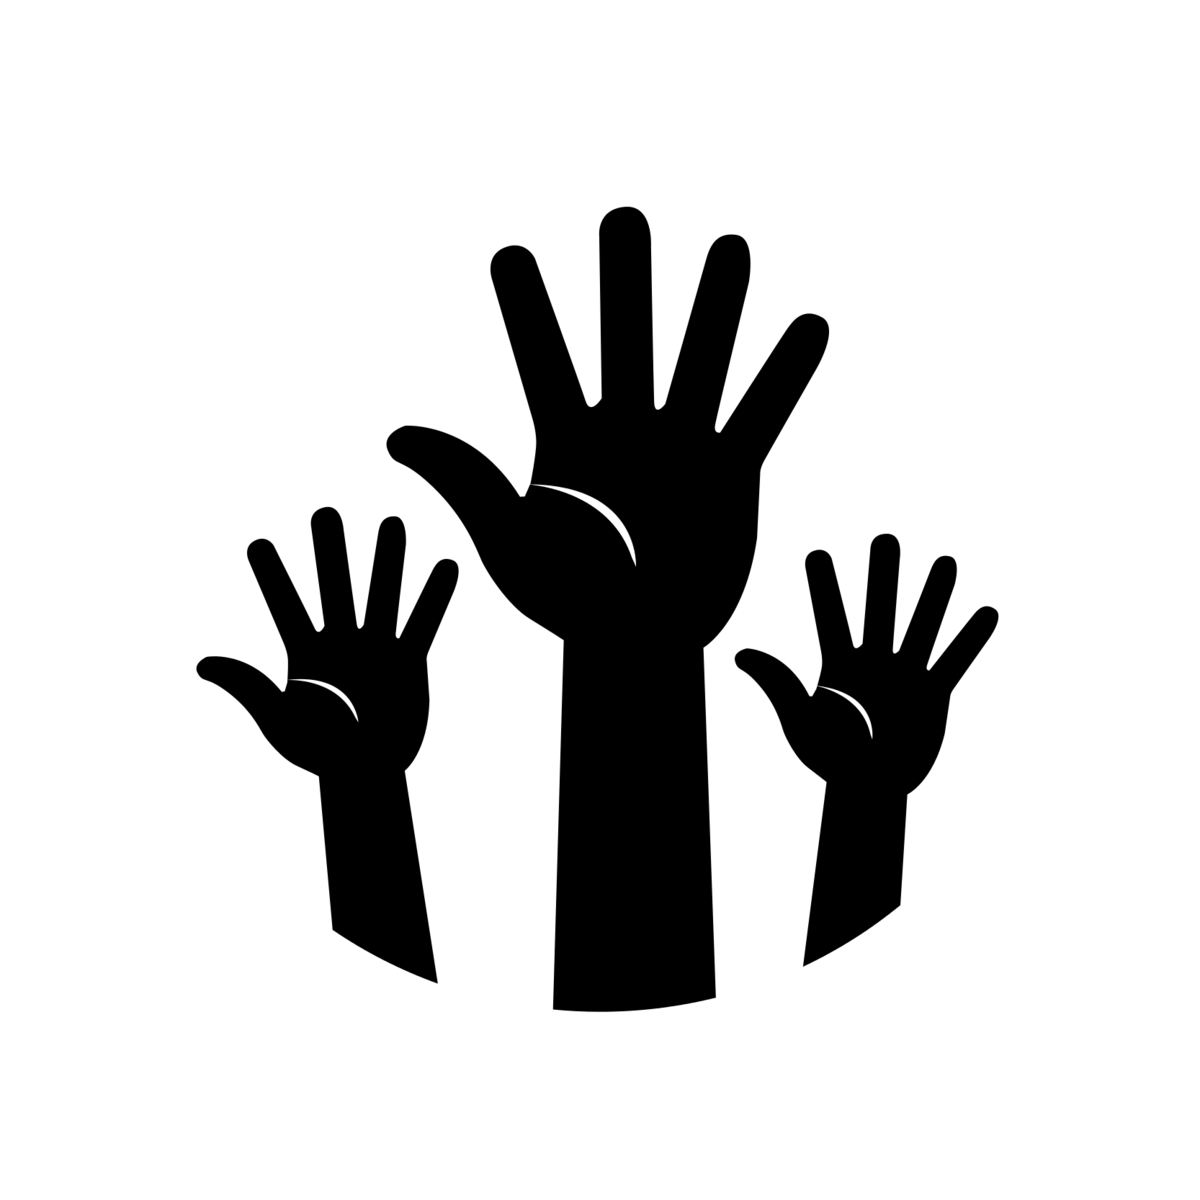
\includegraphics[height=1cm]{images/hands.png}

\bigskip
\pause

\begin{itemize}
  \item Grid search
  \item Random search
  \item Stochastic local search algorithms
  \item Genetic algorithms
  \item Constraint satisfaction problem
  \begin{itemize}
    \item Mixed-Integer Programming
    \item Answer Set Programming
  \end{itemize}
  \item \ldots
\end{itemize}


\end{frame}
%-----------------------------------------------------------------------
%----------------------------------------------------------------------
\begin{frame}[c]{Time-minimal Algorithm Alignment}

\begin{definition}
Given a portfolio (set) of algorithms $\portfolio$, a set of instances $\insts$,
runtime as a cost metric $t: \portfolio \times \insts \to \perf$,
a runtime cutoff $\kappa$,
and an unordered schedule~$\sigma$,
the time-minimal algorithm alignment problem is to find a permutation $\rho$ such that:

	\begin{eqnarray*}
	  \rho
	  & \in & 
	  \argmin_{\rho:\{1,\dots,|\portfolio|\}\rightarrow \portfolio}
	  \textstyle{\sum}_{\inst \in \insts}
	  \tau_{\sigma,\rho}(\inst)\\
%----------------------
	  \tau_{\sigma,\rho}(\inst) & = &
	    \begin{cases} 
	      \left(
	        \textstyle{\sum}_{j=1}^{\min{(P)} - 1}
	        \sigma(\rho(j))
	      \right)
	      +
	      t(\rho(\min{(P)}),\inst)
	       & \text{if $P \not= \emptyset$,}\\
	      \kappa & \text{otherwise}
	    \end{cases}\\
%-----------------------------------
	P & = & \{ l \in \{1,\dots,|\portfolio|\} \mid t(\rho(l),\inst)\leq\sigma(\rho(l)) \}
	\end{eqnarray*}
\end{definition}

\end{frame}
%-----------------------------------------------------------------------
%----------------------------------------------------------------------
\begin{frame}[c,fragile]{Time-minimal Algorithm Alignment: Pseudo-Code}

Pseudo-Python-code to score a permutation $\rho$ given a time slice assignment $\sigma$
and an algorithm portfolio $\portfolio$ of size $k$:

\begin{semiverbatim}
time = 0
for \inst \in \insts:
  for \emph{l} in range(1,k+1):
    if t(\rho(l),\inst) \leq \sigma(\rho(l)):
        time += t(\rho(l),\inst)
        break
    else:
        time += \sigma(\rho(l))
\end{semiverbatim}

\end{frame}
%-----------------------------------------------------------------------
%----------------------------------------------------------------------
\begin{frame}[c]{Algorithm Schedules}

Schedule: $\sigma = \{\algo_1 \mapsto 1, \algo_3 \mapsto 2, \algo_2 \mapsto 7\}$\\
$\rho = \{1 \mapsto \algo_1, 2 \mapsto \algo_3, 3 \mapsto \algo_2\}$


\[
\begin{array}{| r | c  c  c || c | c c |}
  \cline{1-7}
      & \algo_1 & \algo_2 & \algo_3 & oracle & Seq. \portfolio & \sigma\\
  \cline{1-7}
  \inst_1 & 		 1    &         10  &         3    & 1  & 3 & 1\\
  \inst_2 &          5    &         10  &  		2 	  & 2 & 6 & 3\\
  \inst_3 &          8    &  		1    &         10  & 1 & 3 & 4\\
  \inst_4 &         10  &         10  & 		2 	  & 2 & 6 & 3\\
  \inst_5 &         10  & 		 6    &         10  & 6 & 10 & 9\\
  \inst_6 &         10  &          8    &         10  & 8 & 10 & 10\\
  \cline{1-7}
  \varnothing & 7.3 & 7.5 & 6.1 & 3.3 & 6.3 & 5\\
  \cline{1-7}
  \text{timeouts} & 3 & 3 & 3 & 0 & 2 & 1\\ 
  \cline{1-7}
\end{array}
\]

On instance $\inst_2$:\\
$P = \{2\}$\\
\pause
$\tau_{\sigma, \rho} = \sigma(\rho(1)) + t(\inst_2, \rho(2)) = 1 + 2 = 3$

\end{frame}
%-----------------------------------------------------------------------
%----------------------------------------------------------------------
\begin{frame}[c]{Schedules Examples~\litw{Hoos et. al 2015}}

\centering
\begin{tabular}{ l | c  c  c  }
\toprule
   & SAT Crafted & SAT mixed & ASP\\
 \midrule
 Cutoff (sec.) & $5000$ & $5000$ & $900$ \\
 \#Instances  & $300$ & $5467$ & $2432$\\
 \#Algorithms  & $15$ & $37$ & $25$ \\
\bottomrule
\end{tabular}

\bigskip
\pause

\begin{tabular}{ l | r r | r r | r r }
\toprule
 & \multicolumn{2}{c}{SAT Crafted} & \multicolumn{2}{c}{SAT mixed} & \multicolumn{2}{c}{ASP}\\
 \midrule
 Single Best  						& $155$ & $(51.6\%)$ & $1881$ & $(34.4\%)$ & $290$ & $(11.9\%)$\\
 Seq. Schedule       				& $123$ & $(41.0\%)$ & $1001$ & $(18.3\%)$ & $280$ & $(11.5\%)$ \\ 
 \alert{opt. Schedule}				& $98$  & $(32.6\%)$ & $536$ & $(9.8\%)$ & $134$ & $(5.5\%)$\\
 \onslide<3->{\alert{par. Schedule (8)} & $85$  & $(28.3\%)$ & $140$ & $(2.5\%)$ & $56$ & $(2.3\%)$}\\
\bottomrule
\end{tabular}
Number of timeouts (percentage of timeouts)

\end{frame}
%-----------------------------------------------------------------------
%----------------------------------------------------------------------
\begin{frame}[c]{Dynamic Algorithm Portfolios~\litw{Gagliolo and Schmidhuber 2007}}

\begin{block}{Idea}
\begin{itemize}
  \item Collecting training data can be expensive
  \item[$\leadsto$] Try to learn schedule on-the-fly
  \item Adapting time slices over time can be seen as\\ multi-armed bandit problem
\end{itemize}
\end{block}

\pause

\begin{block}{In a nutshell: Multi-Armed Bandit Problem}
\begin{center}
  \includegraphics[width=2.5em]{images/Multi-armed-bandit}
  \includegraphics[width=2.5em]{images/Multi-armed-bandit}
  \includegraphics[width=2.5em]{images/Multi-armed-bandit}
  \includegraphics[width=2.5em]{images/Multi-armed-bandit}
  \includegraphics[width=2.5em]{images/Multi-armed-bandit}
\end{center}
\vspace{-2em}
\begin{itemize}
  \item you are in a casino and have to decide which machine (i.e., arm) to play, how many times and in which order
  \item Each machines provides reward drawn from unknown distribution
  \item Reward distributions are specific to the machine
  \item[$\leadsto$] Trade-off between exploration and exploitation
\end{itemize}
\end{block}

\end{frame}
%-----------------------------------------------------------------------
%----------------------------------------------------------------------
\begin{frame}[c]{Dynamic Algorithm Portfolios~\litw{Gagliolo and Schmidhuber 2007}}

\begin{block}{Idea (cont'd)}
\begin{itemize}
  \item Algorithms are arms in this setting
  \item[$\leadsto$] Play promising arms more often\\ $\approx$ larger time slices for promising algorithms  
\end{itemize}

\pause

\begin{enumerate}
  \item start with a uniform algorithm schedule
  \item for each problem instance $\inst$:
  \begin{enumerate}
    \item run each algorithms $\algo$ with time slice $\sigma(\algo)$ on instance $\inst$
    \item update time slices $\sigma$
    \item if an algorithm solved $\inst$, break
  \end{enumerate}
\end{enumerate}

\pause

Notes: Approach can be improved 
\begin{itemize}
  \item if state of each algorithm is available 
  %\item if intermediate reward signals are available
  \item if similarity between instances is known
\end{itemize}

\end{block}


\end{frame}
%-----------------------------------------------------------------------
%----------------------------------------------------------------------
\begin{frame}[c]{Algorithm Selection~\litw{Rice 1976}}

\begin{block}{Definition}
Given 
\begin{itemize}
  \item a set $\insts$ of problem instances,
  \item a portfolio of algorithms $\portfolio$,
  \item and a cost metric $c:  \portfolio \times \insts \rightarrow \perf$,   
\end{itemize}
 
the \emph{per-instance algorithm selection problem} is to find a mapping 
$s: \insts \rightarrow \portfolio$ 
that optimizes $\sum_{\inst \in \insts} m(s(\inst),\inst)$, 
the sum of performance measures achieved by running the selected algorithm $s(\inst)$ for instance~$\inst$.
\end{block}

\bigskip

\scalebox{0.8}{
\tikzstyle{activity}=[rectangle, draw=black, rounded corners, text centered, text width=8em, fill=white, drop shadow]
\tikzstyle{data}=[rectangle, draw=black, text centered, fill=black!10, text width=8em, drop shadow]
\tikzstyle{myarrow}=[->, thick]
\begin{tikzpicture}[align=center,node distance=3.7cm, thick]
	%PreProcessing
	%\node (PreSolving) [activity, right of=Instance] {Run Pre-Solving Schedule};
	\node (Features) [activity] {Compute\\ Features $\feat(\inst)$};
	\node (Instance) [data, left of=Features] {Instance $\inst$};
	\node (Select) [activity, right of=Features] {Select Algorithm\\ $\feat(\inst) \mapsto \hat{a}$};
	\node (Solve) [activity, right of=Select] {Run $\hat{a}$ on $\inst$};
	\node (Portfolio) [data, above of=Select, yshift=-2.0cm] {Algorithm Portfolio $\portfolio$};

	\draw[myarrow] (Instance) -- (Features);
	%\draw[myarrow] (PreSolving) -- (Features);
	\draw[myarrow] (Features) -- (Select);
	\draw[myarrow] (Select) -- (Solve);
	\draw[myarrow] (Portfolio) -- (Select);
	%\draw[myarrow] (Portfolio) -- (PreSolving);

\end{tikzpicture}
}

\bigskip
\pause
Note: Collecting the training data for the selector can be quite expensive.

\end{frame}
%-----------------------------------------------------------------------
%----------------------------------------------------------------------
\begin{frame}[c]{Instance Features}

\begin{block}{Counting Features}
By analyzing an instance, we can compute some statistics about its characteristics. \\
\end{block}

\bigskip

\begin{block}{Probing Features}
By running an algorithm on an instance for a short amount of time,
we can analyze how the algorithm behaves on this instance.\\
\end{block}

\bigskip
\pause

Please note that there a different names in literature for these types of features.
For example, probing features are related to landmarking features.

\end{frame}
%-----------------------------------------------------------------------
%----------------------------------------------------------------------
\begin{frame}[c]{Instance features: Machine Learning}

\begin{center}
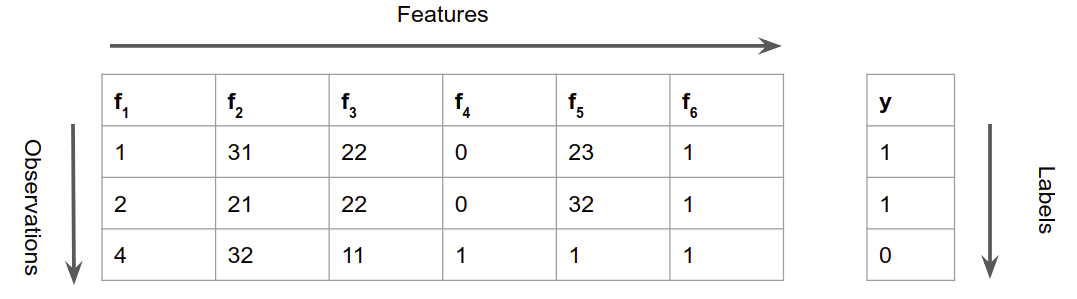
\includegraphics[width=0.9\textwidth]{images/ml_data}
\end{center}


What kind of ``instance features'' could describe a dataset? \hands

\pause
\begin{itemize}
  \item number of observations (samples)
  \item number of features
  \item number of classes
  \item number of categorical features
  \item number of numeric features
  \item percentage of numeric features
  \item number of missing features
  %\item number of observations belonging to most frequent class
  \item Probing: accuracy of a small decision tree
\end{itemize}

\end{frame}
%-----------------------------------------------------------------------
%----------------------------------------------------------------------
\begin{frame}[c]{Instance Features: SAT}

Boolean satisfiability (SAT) instances are encoded as\\ conjunctions of disjunctions of Boolean variables:

$(x_1 \vee x_2)\wedge (x_2 \vee x_3 \vee \neg x_4) \wedge (\neg x_1 \vee x_4) \wedge (\neg x_2 \vee \neg x_3)$

\medskip
\pause
What kind of ``instance features'' could describe such a formula? \hands

\medskip
\pause
\begin{itemize}
  \item number of variables?
  \item number of conjunctions (a.k.a. clauses)
  \item ratio of number of variables and number of clauses
  \pause
  \item Probing feature: number of unsatisfied clauses after running SAT solver for a few seconds 
  \item \ldots
\end{itemize}


\end{frame}
%-----------------------------------------------------------------------
%----------------------------------------------------------------------
\begin{frame}[c]{Instance Features: SAT}

\begin{itemize}
  \item Problem size features (7)
  \item Variable-Clause graph features (10)
  \item Variable graph features (9) (expensive)
  \item Clause graph features (10) (expensive)
  \item Balance features (13)
  \item Proximity to horn formula (7) (expensive)
  \item DPLL Probing Features (7)
  \item LP-based feature (6) (moderate)
  \item Local search probing features (12) (cheap)
  \item Clause learning features (18) (cheap)
  \item Survey propagation feature (18) (moderate)
\end{itemize}

\lit{Algorithm Runtime Prediction: Methods \& Evaluation by Hutter et al. 2014}

\end{frame}
%-----------------------------------------------------------------------
%----------------------------------------------------------------------
\begin{frame}[c]{Instance Features: Runtime~\litw{Xu et al. 2008}}

\centering
\includegraphics[width=1\textwidth]{images/random_indu_feature_rtd.png}

on random instances \hspace{2.2cm}  on industrial instances\

\bigskip
\pause

\flushleft
$\to$ feature computation can be expensive on some instances\\
$\to$ use feature selection to determine an informative but cheap set of features

\end{frame}
%-----------------------------------------------------------------------

%----------------------------------------------------------------------
% \begin{frame}[c]{How to implement an algorithm selector?}
% 
% \begin{center}
% 
\includegraphics[height=1cm]{images/discussion.png}
% \end{center}
% 
% \end{frame}
%-----------------------------------------------------------------------
%----------------------------------------------------------------------
\begin{frame}[c]{\satzilla{}~\litw{Xu et al. 2009}}

\begin{itemize}
  \item one of the prominent approaches for algorithm selection in SAT
  \item won several first places in the SAT competition
  \medskip
  \item Simple idea:
  \begin{enumerate}
    \item use a static algorithm schedule (called pre-solving schedule)
    \item if the pre-solving schedule failed to solve the instance at hand,\\
    		compute the instance features of the instance
    \item run the algorithm with the best predicted performance
    	  \begin{itemize}
    	    \item use a regression model to predict the performance of each algorithm\\
    	    ($\to$ $k$ regression models for $k$ algorithms in the portfolio)
    	  \end{itemize}
  \end{enumerate}
\end{itemize}

\end{frame}
%-----------------------------------------------------------------------
%----------------------------------------------------------------------
\begin{frame}[c]{Literature}

\begin{itemize}
  \item \lit{SATzilla: Portfolio-based Algorithm Selection for SAT. L. Xu, F. Hutter, H. H. Hoos, K. Leyton-Brown - Journal of Artificial Intelligence Research, Volume 32, pp. 565–606, 2008}
  \item \lit{Lars Kotthoff. Algorithm Selection for Combinatorial Search Problems: A Survey. AI Magazine, 2014}
  \item Literature overview: \url{http://larskotthoff.github.io/assurvey/}
\end{itemize}


\end{frame}
%-----------------------------------------------------------------------
%----------------------------------------------------------------------
\begin{frame}[c]{Learning Goals}

After this lecture, you will be able to \ldots

\begin{itemize}
  \item \alert{exploit complementarity} of algorithms to improve overall performance
  \item explain \alert{algorithm portfolios} and its different variants
  \begin{itemize}
    \item racing portfolios
    \item parallel portfolios
    \item algorithm schedules
  \end{itemize}
  \item define \alert{per-instance algorithm selection} and to describe one specific implementation 
  \item explain different types of \alert{instance features}
\end{itemize}

\end{frame}
%-----------------------------------------------------------------------
%%----------------------------------------------------------------------
\begin{frame}[c]{Where are we? The big picture}

\begin{itemize}
\item Algorithm Selection
  \begin{itemize}
    \item Portfolios
    \item Algorithm selection (for runtime)
  \end{itemize}
  \item[$\to$] Design Decisions:\\ Local Search + Evo. Algorithms + Machine Learning 
  \item Empirical evaluation
  \item AAD for ML
  \begin{itemize}
    \item Hyperparameter optimization and Bayesian Optimization 
    \item Neural architecture search (lecture given by Prof. Hutter)
  \end{itemize}
  \item Algorithm configuration 
  \begin{itemize}
    \item Basics 
    \item State of the art 
    \item Best Practices 
  \end{itemize}
  \item Combinations of algorithm selection and configurations
  \item Algorithm control 
  \item Algorithm analysis 
  \item Project announcement and questions for exam 
\end{itemize}

\end{frame}
%----------------------------------------------------------------------
%----------------------------------------------------------------------
\begin{frame}[c]{Preview: Learning Goals}

What will we learn today?

\begin{enumerate}
  \item Recap: Optimization algorithms
  \begin{itemize}
    \item Stochastic local search (SLS)
    \item Evolutionary algorithms
  \end{itemize}
  \item Recap: Machine learning algorithms
  \begin{itemize}
    \item kNN, tree-based algorithms, neural networks
  \end{itemize}
  \item What are typical decisions in algorithm design?
  \medskip
  \item[$\leadsto$] The algorithms discussed today will also be important\\ in later sessions of the course! 
\end{enumerate}

\end{frame}
%-----------------------------------------------------------------------
%----------------------------------------------------------------------
\begin{frame}[c]{}

\vspace{2cm}
\centering
{\huge
Solving Combinatorial Problems:\\
Stochastic Local Search (SLS)
}

\vspace{3cm}
Material partially from\\ ``Stochastic Local Search: Foundations and Applications''\\ by Hoos and Stützle
\end{frame}
%----------------------------------------------------------------------
%----------------------------------------------------------------------
\begin{frame}[c]{Global View on Problems}


\begin{center}
\includegraphics[height=5cm]{images/f01-03-left}
\parbox[t]{5.5cm}{
        \vspace*{-4.5cm}
        \begin{itemize}
        \item vertices: candidate solutions (search positions)
        \bigskip
        \item edges: connect neighbouring positions
        \bigskip
        \onslide<2->
        \item s: (optimal) solution
        \bigskip
        \item c: current search position
        \end{itemize}
}
\end{center}

\note{Birds-eye view of search space}
\end{frame}
%-----------------------------------------------------------------------
%----------------------------------------------------------------------
\begin{frame}[c]{Local View on Problems}

\begin{center}
\includegraphics[height=5cm]{images/f01-03-right}
\end{center}

\bigskip
Next search position is selected from local neighbourhood
  based on local information, \eg{}, heuristic values.

\end{frame}
%-----------------------------------------------------------------------
%----------------------------------------------------------------------
\begin{frame}[c]{Stochastic Local Search}

\onslide<+->
{Many prominent local search algorithms use
\alert{randomized choices} in generating
and modifying candidate solutions.
}

\medskip

\onslide<+->
These \alert{stochastic local search (SLS) algorithms}
are one of the most successful and widely used approaches
for solving hard combinatorial problems.

\medskip

\begin{block}<+->{Some well-known SLS methods and algorithms:}
\begin{itemize}
\item Tabu search, simulated annealing, iterated local search,\\ dynamic local search, \ldots
\end{itemize}
\end{block}

\end{frame}
%-----------------------------------------------------------------------
% %----------------------------------------------------------------------
% \begin{frame}[c]{Definition: SLS}
% 
% For given problem instance $\pi$:
% \begin{itemize}
% \medskip
% \item<+->\alert{search space $S(\pi)$}\\
%         (\eg{}, for SAT: set of all complete truth assignments \\
%         to propositional variables)
% \medskip
% \item<+->\alert{solution set $S'(\pi) \subseteq S(\pi)$}\\
%         (\eg{}, for SAT: models of given formula)
% \medskip
% \item<+->\alert{neighbourhood relation $N(\pi) \subseteq S(\pi) \times S(\pi)$}\\
%         (\eg{}, for SAT: neighbouring variable assignments differ \\
%         in the truth value of exactly one variable)
% \end{itemize}
% 
% \end{frame}
% %-----------------------------------------------------------------------
% %----------------------------------------------------------------------
% \begin{frame}[c]{Definition: SLS}
% 
% \begin{itemize}
% \item<+->\alert{set of memory states $M(\pi)$}\\
%         (may consist of a single state for SLS algorithms that \\
%                 do not use memory)
% \medskip
% \item<+->\alert{initialization function $\mbox{\sl init}: 
%         \emptyset \mapsto {\cal D}(S(\pi) \times M(\pi))$}\\
%         (specifies probability distribution over initial search positions
%                 and memory states)
% \medskip
% \item<+->\alert{step function $\mbox{\sl step}: 
%         S(\pi) \times M(\pi) \mapsto {\cal D}(S(\pi) \times M(\pi))$}\\
%         (maps each search position and memory state onto \\
%                 probability distribution over subsequent, neighbouring \\
%                 search positions and memory states)
% \medskip
% \item<+->\alert{termination predicate $\mbox{\sl terminate}: 
%         S(\pi) \times M(\pi) \mapsto {\cal D}(\{\top,\bot\})$}\\
%         (determines the termination probability for each \\
%                 search position and memory state)
% \end{itemize} 
% 
% \end{frame}
% %-----------------------------------------------------------------------
%----------------------------------------------------------------------
% \begin{frame}[c]{SLS for Decision Problems}
% 
% \begin{columns}
% 
% \column{0.5\textwidth}
% 
% {\small
% \hspace*{0cm}
% \parbox{0cm}{
% \begin{tabbing}
% ----\=----\=----\=----\=----\=----\=----\=----\=\kill
% \onslide<1->
% \pscProc\ {\em SLS-Decision$(\pi)$}\\
% \> {\bf input:} {\em problem instance} $\pi \in \Pi$\\
% \> {\bf output:} {\em solution} $s \in S'(\pi)$ {\bf or} $\emptyset$\\[1mm]
% \onslide<2->
% \> $(s,m) := \func{init(\pi)}$;\\
% \\
% \onslide<3->
% \> \pscWhile\ {\bf not} $\func{terminate(\pi,s,m)}$ \pscDo\\
% \> \> $(s,m) := \func{step(\pi,s,m)}$;\\ 
% \> \pscEnd\\
% \ \\
% \ \\
% \ \\
% \onslide<4->
% \> \pscIf\ $s \in {S'(\pi)}$ \pscThen \\
% \> \> \pscReturn\ $s$\\
% \> \pscElse \\
% \> \> \pscReturn\ $\emptyset$\\
% \> \pscEnd\\
% \onslide<1->
% \pscEnd\ {\em SLS-Decision}
% \end{tabbing}
% }
% }
% 
% \column{0.5\textwidth}
% 
% \begin{description}
%  \item[$\pi$] instance
%  \item[$s$] solution candidate
%  \item[$S'$] set of possible solutions 
%  \item[$m$] memory state
%  \item[init] initialization function
%  \item[step] neighborhood function
%  \item[terminate] termination criterion
% \end{description}
% 
% \end{columns}
% 
% 
% 
% \end{frame}
% %-----------------------------------------------------------------------
% %----------------------------------------------------------------------
% \begin{frame}[c]{SLS for Optimization Problems}
% 
% \begin{columns}
% 
% \column{0.5\textwidth}
% 
% {\small
% \hspace*{0cm}
% \parbox{0cm}{
% \begin{tabbing}
% ----\=----\=----\=----\=----\=----\=----\=----\=\kill
% \onslide<1->
% \pscProc\ {\em SLS-Minimization$(\pi')$}\\
% \> {\bf input:} {\em problem instance} $\pi' \in \Pi'$\\
% \> {\bf output:} {\em solution} $s \in S'(\pi')$ {\bf or} $\emptyset$\\[1mm]
% \onslide<1->
% \> $(s,m) := \func{init(\pi')}$;\\
% \> \alert{{$\hat{s} := s$;}}\\
% \onslide<1->
% \> \pscWhile\ {\bf not} $\func{terminate(\pi',s,m)}$ \pscDo\\
% \> \> $(s,m) := \func{step(\pi',s,m)}$;\\ 
% \> \> \alert{{\pscIf\ $f(\pi',s) < f(\pi',\hat{s})$ \pscThen}} \\
% \> \> \> \alert{{$\hat{s} := s$;}}\\
% \> \> \alert{{\pscEnd}}\\
% \> \pscEnd\\
% \onslide<1->
% \> \pscIf\ ${\hat{s}} \in {S'(\pi')}$ \pscThen \\
% \> \> \pscReturn\ {$\hat{s}$}\\
% \> \pscElse \\
% \> \> \pscReturn\ $\emptyset$\\
% \> \pscEnd \\
% \onslide<1->
% \pscEnd\ {\em SLS-Minimization}
% \end{tabbing}
% }
% }
% 
% \column{0.5\textwidth}
% 
% \begin{description}
%  \item[$\pi$] instance
%  \item[$s$] solution candidate
%  \item[$S'$] set of possible solutions 
%  \item[$m$] memory state
%  \item[$f$] function to be optimized
%  \item[init] initialization function
%  \item[step] neighborhood function
%  \item[terminate] termination criterion
% \end{description}
% 
% \end{columns}
% 
% \end{frame}
% %-----------------------------------------------------------------------
%----------------------------------------------------------------------
\begin{frame}[c]{Applications of SLS?}

\centering
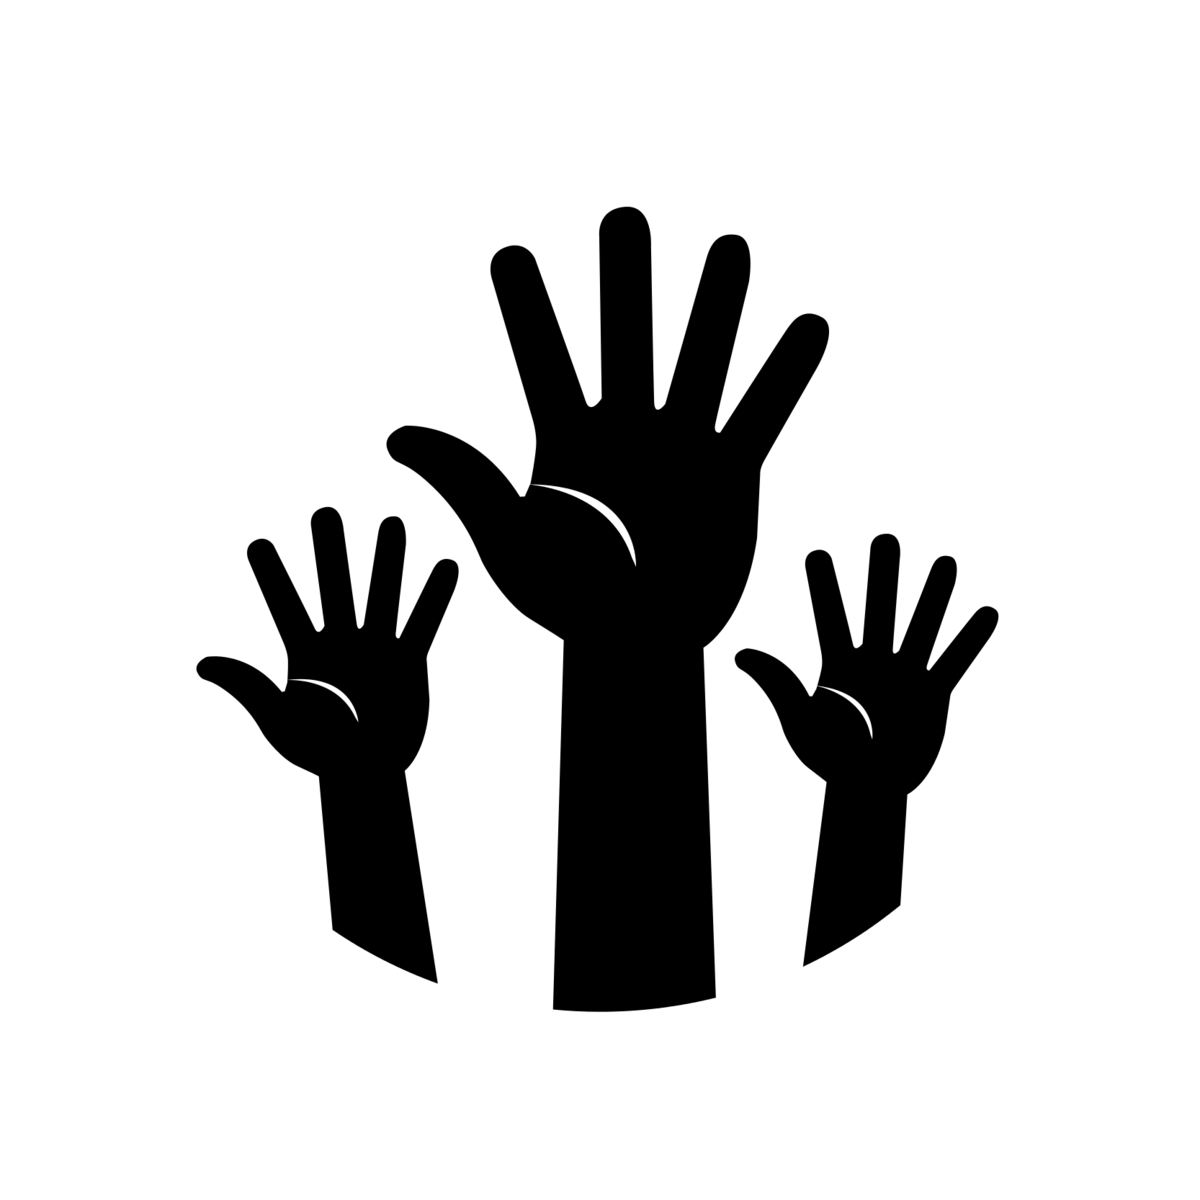
\includegraphics[scale=.1]{images/hands.png}

\end{frame}
%-----------------------------------------------------------------------
%----------------------------------------------------------------------
\begin{frame}[c]{Local Search: Uninformed random walk for SAT}

\begin{block}{SAT}
Boolean satisfiability (SAT) instances are encoded as\\ conjunctions of disjunctions of Boolean variables:

$(x_1 \vee x_2)\wedge (x_2 \vee x_3 \vee \neg x_4) \wedge (\neg x_1 \vee x_4) \wedge (\neg x_2 \vee \neg x_3)$
\end{block}

\pause

{\footnotesize
\begin{tabbing}
----\=----\=----\=----\=----\=----\=----\=----\=\kill
\pscProc\ {\em URW-for-SAT$(F,\mbox{\emph{maxSteps}})$}\\
\> {\bf input:} {\em propositional formula} $F$, \emph{integer} \emph{maxSteps}\\
\> {\bf output:} {\em model of $F$} {\bf or} $\emptyset$\\[1mm]
\onslide<2->
\> choose assignment $a$ of $F$ uniformly at random;\\
\> \emph{steps} := 0; \\
\onslide<3->
\> \pscWhile\ \pscNot(($a$ satisfies $F$)) \pscAnd{}
         (\emph{steps} $<$ \emph{maxSteps}) \pscDo\\
\onslide<4->         
\> \> randomly select variable $x$ in $F$;\\ 
\> \> change value of $x$ in $a$;\\ 
\> \> \emph{steps} := \emph{steps}$+1$;\\
\onslide<5->
\> \> \pscIf\ $a$ satisfies $F$ \pscThen \\
\> \> \> \pscReturn\ $a$\\
\> \pscEnd\\
\onslide<6->
\> \pscReturn\ $\emptyset$\\
\pscEnd\ {\em URW-for-SAT}
\end{tabbing}
}
\end{frame}
%-----------------------------------------------------------------------
%----------------------------------------------------------------------
\begin{frame}[c]{Example: URW for SAT}

\centering

$F:= (\neg x_1 \vee x_2) 
		\wedge (\neg x_2 \vee x_1) 
		\wedge (\neg x_1 \vee \neg x_2 \vee \neg x_3) 
		\wedge ( x_1 \vee x_2) 
		\wedge (\neg x_4 \vee x_3) 
		\wedge(\neg x_5 \vee x_3) 
$

\bigskip

\begin{tabular}{lccccc}
Step & $x_1$ & $x_2$ & $x_3$ & $x_4$ & $x_5$ \\ 
\hline
1 & $\top$ & $\top$ & $\top$ & $\top$ & $\top$ \\
\pause
2 & $\bot$ & $\top$ & $\top$ & $\top$ & $\top$ \\
\pause
3 & $\bot$ & $\top$ & $\bot$ & $\top$ & $\top$ \\
\pause
4 & $\bot$ & $\top$ & $\bot$ & $\top$ & $\bot$ \\
\pause
5 & $\bot$ & $\top$ & $\bot$ & $\top$ & $\top$ \\
\pause
6 & $\bot$ & $\top$ & $\bot$ & $\bot$ & $\top$ \\
\pause
7 & $\bot$ & $\top$ & $\bot$ & $\bot$ & $\bot$ \\
\pause
8 & $\top$ & $\top$ & $\bot$ & $\bot$ & $\bot$ \\
\end{tabular}

\end{frame}
%-----------------------------------------------------------------------
%----------------------------------------------------------------------
% \begin{frame}[c]{URW for SAT}
% 
% \begin{itemize}
% \item {\bf search space $S$:} set of all truth assignments to variables \\
%                 in given formula $F$
% 
% \medskip
% 
% \item {\bf solution set $S'$:} set of all models of $F$
% 
% \medskip
% 
% \onslide<2->
% \item {\bf neighbourhood relation $N$:} \emph{1-flip neighbourhood},
%         \ie{}, assignments are neighbours under $N$     iff they differ in \\
%         the truth value of exactly one variable
% 
% \bigskip
% 
% \onslide<3->
% \item {\bf memory:} not used, \ie{}, $M := \{0\}$
% \end{itemize}
% 
% \end{frame}
% %-----------------------------------------------------------------------
% %----------------------------------------------------------------------
% \begin{frame}[c]{URW for SAT}
% 
% \begin{itemize}
% \item {\bf initialization:} 
%         uniform random choice from $S$, 
%         \ie{}, $\func{init}(): (a',m) := 1/\#S$ for all assignments $a'$ and \\
%                 memory states $m$
% 
% \medskip
% 
% \onslide<2->
% \item {\bf step function:} uniform random choice from current neighbourhood,
%   \ie{}, $\func{step}(a,m): (a',m) := 1/\#N(a)$ \\
%     for all assignments $a$ and memory states $m$, \\
%     where $N(a) := \{a' \in S \mid N(a,a')\}$ is the set of \\
%     all neighbours of $a$.
% 
% \medskip
% 
% \onslide<3->
% \item {\bf termination:} when model is found, \ie{}, \\
%         $\func{terminate}(a,m):(\top) := 1$ if $a$ is a model of $F$,
%                 and $0$ otherwise.
% \end{itemize}
% 
% \end{frame}
%-----------------------------------------------------------------------
%-----------------------------------------------------------------------
\begin{frame}[c]{Improvements of URW?}

{\footnotesize
\begin{tabbing}
----\=----\=----\=----\=----\=----\=----\=----\=\kill
\pscProc\ {\em URW-for-SAT$(F,\mbox{\emph{maxSteps}})$}\\
\> {\bf input:} {\em propositional formula} $F$, \emph{integer} \emph{maxSteps}\\
\> {\bf output:} {\em model of $F$} {\bf or} $\emptyset$\\[1mm]
\> choose assignment $a$ of $F$ uniformly at random;\\
\> \emph{steps} := 0; \\
\> \pscWhile\ \pscNot(($a$ satisfies $F$) \pscAnd{}
         (\emph{steps} $<$ \emph{maxSteps})) \pscDo\\
\> \> randomly select variable $x$ in $F$;\\ 
\> \> change value of $x$ in $a$;\\ 
\> \> \emph{steps} := \emph{steps}$+1$;\\
\> \> \pscIf\ $a$ satisfies $F$ \pscThen \\
\> \> \> \pscReturn\ $a$\\
\> \pscEnd\\
\> \pscReturn\ $\emptyset$\\
\pscEnd\ {\em URW-for-SAT}
\end{tabbing}
}

\centering
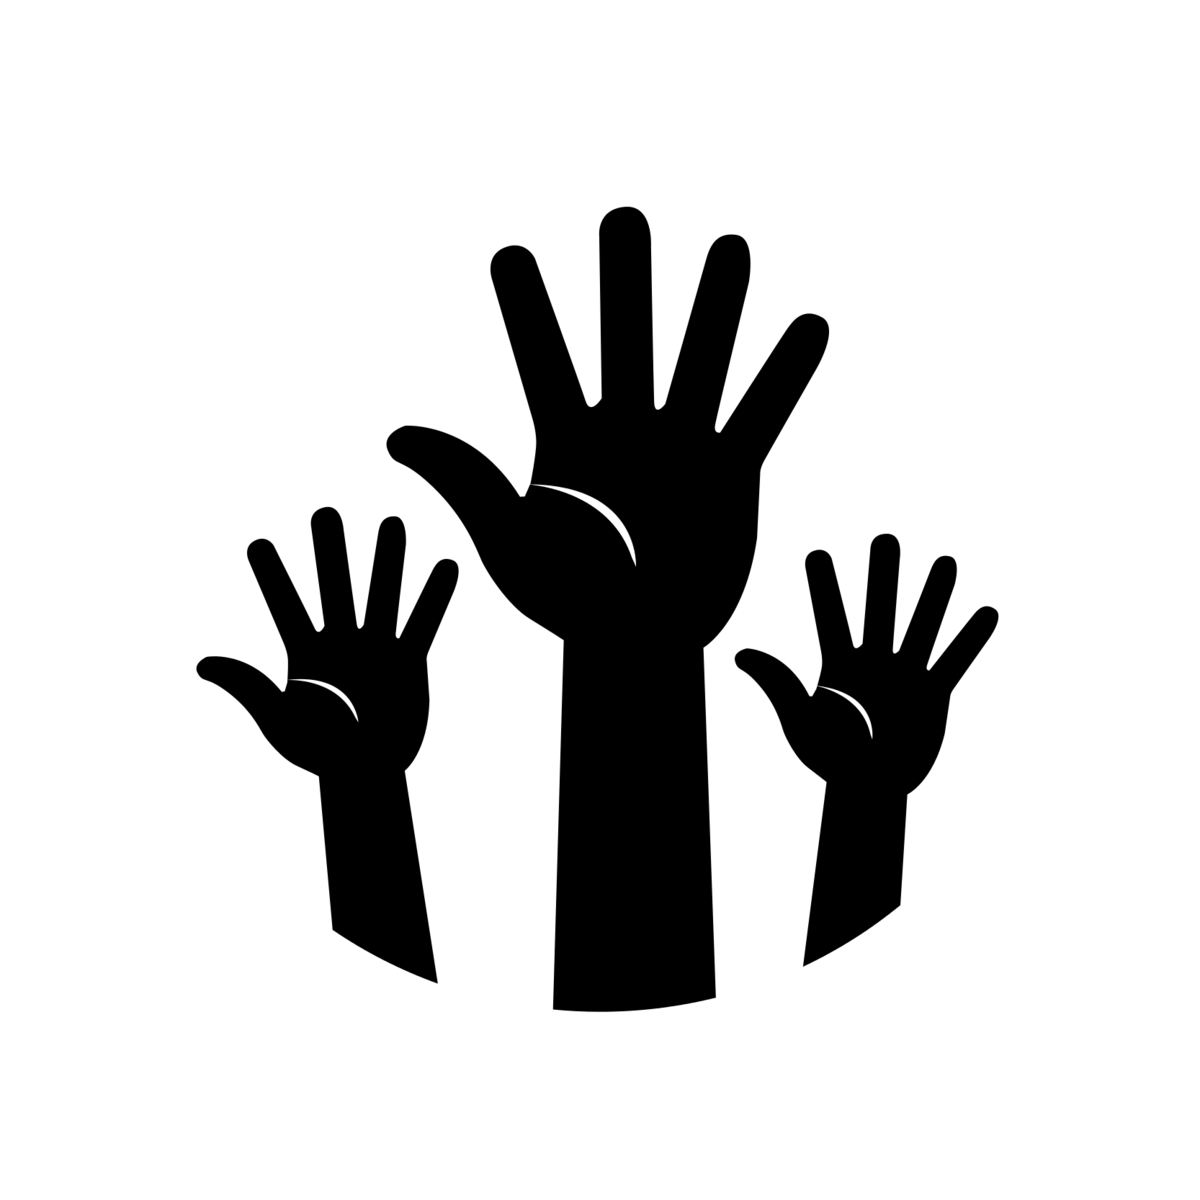
\includegraphics[scale=.05]{images/hands.png}

\end{frame}
%-----------------------------------------------------------------------
%-----------------------------------------------------------------------%-----------------------------------------------------------------------
\begin{frame}[c]{Evaluation function}

\onslide<+->
\begin{block}{Evaluation function:}
\begin{itemize}
\item function $g(\pi): S(\pi) \mapsto \Reals$ that maps candidate solutions of \\
        a given problem instance $\pi$ onto real numbers, \\
        such that global optima correspond to solutions of $\pi$;
\onslide<+->
\item used for ranking or assessing neighbours of current \\
        search position to provide guidance to search process.
\end{itemize}
\end{block}

\medskip

\onslide<+->
\begin{block}{Evaluation \vs{} objective functions:}
\begin{itemize}
\item \emph{Evaluation function}: part of SLS algorithm.
\item \emph{Objective function}: integral part of optimization problem.
\onslide<+->
\item Some SLS methods use evaluation functions different from
        given objective function (\eg{}, dynamic local search).
\end{itemize}
\end{block}

\end{frame}
%-----------------------------------------------------------------------
% %-----------------------------------------------------------------------
% \begin{frame}[c]{Iterative Improvement (II)}
% 
% \onslide<+->
% \begin{itemize}
% \item does not use memory
% \item $\func{init}$: uniform random choice from $S$
% 
% \onslide<+->
% \item $\func{step}$: uniform random choice from improving neighbours, \\
%         \ie{}, $\func{step}(s): (s') := 1/\#I(s)$ if $s' \in I(s)$,
%         and $0$ otherwise, \\
%         where $I(s) := \{s' \in S \mid N(s,s') \wedge g(s') < g(s)\}$
% 
% \medskip
%         \onslide<+->
% \item terminates when no improving neighbour available\\
%         (to be revisited later)
% \medskip
%         \onslide<+->
% \item different variants through modifications of step function\\
%         (to be revisited later)
% 
% \end{itemize}
% 
% \medskip
% 
% \onslide<+->
% \emph{Note:} II is also known as \emph{iterative descent}
%         or \emph{hill-climbing}.
% 
% \end{frame}
% %-----------------------------------------------------------------------
% %-----------------------------------------------------------------------
% \begin{frame}[c]{Iterative Improvement for SAT}
% 
% 
% \begin{itemize}
% \item {\bf search space $S$:} set of all truth assignments to variables \\
%                 in given formula $F$
% \item {\bf solution set $S'$:} set of all models of $F$
% \item {\bf neighbourhood relation $N$:} 1-flip neighbourhood \\
%         (as in Uninformed Random Walk for SAT)
% 
% \medskip
% 
% \onslide<+->
% \item {\bf memory:} not used, \ie{}, $M := \{0\}$
% 
% \item {\bf initialization:} 
%         uniform random choice from $S$, 
%         \ie{}, $\func{init}() : (a',m) := 1/\#S$ for all assignments $a'$\\
%         and memory states $m$
% 
% \end{itemize}
% 
% \end{frame}
% %-----------------------------------------------------------------------
% %-----------------------------------------------------------------------
% \begin{frame}[c]{Iterative Improvement for SAT}
% 
% \begin{itemize}
% \item {\alert
%         {\bf evaluation function:} $g(a) := $ number of clauses in $F$ \\
%         that are \emph{unsatisfied} under assignment $a$\\
%         }
%         (\emph{Note:} $g(a)=0$ iff $a$ is a model of $F$.)
%   
% 
% \medskip
% 
% \onslide<+->
% \item {\bf step function}: uniform random choice from improving neighbours,
%         \ie{}, $\func{step}(a)(a') := 1/\#I(a)$ if $s' \in I(a)$, \\
%         and $0$ otherwise,
%         where $I(a) := \{a' \mid N(a,a') \wedge g(a') < g(a)\}$
% 
% \medskip
% 
% \onslide<+->
% \item {\bf termination}: when no improving neighbour is available \\
%         \ie{}, $\func{terminate}(a)(\top):=1$ if $I(a)=\emptyset{}$,
%                 and $0$ otherwise.
% \end{itemize}
% 
% \onslide<+->
% \medskip
% \alert{Problem}: II will get stuck in local minima.
% 
% \end{frame}
% %-----------------------------------------------------------------------
%----------------------------------------------------------------------
\begin{frame}[c]{Iterative Improvement with Local Search: WalkSAT\\ \litw{B. Selman et al. 2006}}

\smallskip
{\footnotesize
\begin{tabbing}
----\=----\=----\=----\=----\=----\=----\=----\=\kill
\pscProc\ {\em WalkSAT$(F,\mbox{\emph{maxSteps}})$}\\
\> {\bf input:} {\em propositional formula} $F$, \emph{integer} \emph{maxSteps}\\
\> {\bf output:} {\em model of $F$} {\bf or} $\emptyset$\\[1mm]
\> choose assignment $a$ of $F$ uniformly at random;\\
\> \pscIf\ $a$ satisfies $F$ \textbf{then return} $a$\\
\> \emph{steps} := 0; \\
\> \pscWhile\ (\emph{steps} $<$ \emph{maxSteps}) \pscDo\\
\> \> randomly select an unsatisfied clause $C$;\\ 
\> \> randomly select a variable $v$ that appears in $C$;\\ 
\> \> change the value of $v$ and keep the change unless it\\
\> \> increases the number of unsatisfied clauses;\\ 
%\> \> randomly select variable $x$ in $F$;\\ 
%\> \> change value of $x$ in $a$;\\ 
\> \> \emph{steps} := \emph{steps}$+1$;\\
\> \> \pscIf\ $a$ satisfies $F$ \textbf{then return} $a$\\
\> \pscEnd\\
\> \pscReturn\ $\emptyset$\\
\pscEnd\ {\em WalkSAT}
\end{tabbing}
}
\end{frame}
%-----------------------------------------------------------------------
%----------------------------------------------------------------------
\begin{frame}[c]{Example: WalkSAT for SAT}

\centering

$F:= (\neg x_1 \vee x_2) 
		\wedge (\neg x_2 \vee x_1) 
		\wedge (\neg x_1 \vee \neg x_2 \vee \neg x_3) 
		\wedge ( x_1 \vee x_2) 
		\wedge (\neg x_4 \vee x_3) 
		\wedge(\neg x_5 \vee x_3) 
$

\bigskip

\begin{tabular}{lcccccc}
Step & $x_1$ & $x_2$ & $x_3$ & $x_4$ & $x_5$ & Confl. Clauses\\ 
\hline
1 & $\top$ & $\top$ & $\bot$ & $\top$ & $\top$ & $C_5,C_6$\\
\pause
2 & $\top$ & $\top$ & $\bot$ & $\top$ & $\bot$ & $C_5$\\
\pause
3 & $\top$ & $\top$ & $\top$ & $\top$ & $\bot$ & $C_3$ $\to$ rejected\\
\pause
4 & $\top$ & $\top$ & $\bot$ & $\bot$ & $\bot$ & $\checkmark$\\
\end{tabular}

\end{frame}
%-----------------------------------------------------------------------
% %-----------------------------------------------------------------------
% \begin{frame}[c]{Global vs. Local Optima}
% 
% \onslide<+->
% \begin{block}{Global Optima}
% A global optimum is a search position $s$ with the optimal value of $g(s)$ in the entire search space.
% \end{block}
% 
% \medskip
% 
% \onslide<+->
% \begin{block}{Local Optima}
% A local optima is a search position $s$ with the best value of $g(s)$ in the neighbourhood of $s$.
% \end{block}
% 
% \medskip
% 
% \onslide<+->
% \begin{block}{Plateau}
% Plateaus is a region of search positions with identical evaluation function values.
% \end{block}
% 
% \end{frame}
% %-----------------------------------------------------------------------
% %-----------------------------------------------------------------------
% \begin{frame}{Global vs. Local Optima}
% 
% Extra Space for diagram 
% 
% \end{frame}
% %-----------------------------------------------------------------------
%-----------------------------------------------------------------------
\begin{frame}[c]{Escaping from local optima}

\onslide<+->
\begin{itemize}
\item \emph{Restart:} re-initialize search\\ whenever a local optimum 
        is encountered.\\
         (Sometimes rather ineffective due to cost of initialization.)

\medskip

\onslide<+->
\item \emph{Non-improving steps}:  allow selection of \\
        candidate solutions with equal or worse evaluation function value,
        \eg{}, using minimally worsening steps.\\
        (Can lead to long walks in \emph{plateaus}.)
        
\end{itemize}

\bigskip

\onslide<+->
\emph{Note:} None of these mechanisms is guaranteed to always \\
        effectively escape from local optima.
        
\end{frame}
%-----------------------------------------------------------------------
% %-----------------------------------------------------------------------
% \begin{frame}[c, fragile]{Task: Improved SLS Algorithms}
% 
% \begin{columns}
% \column{0.6\textwidth}
% 
% \includegraphics[scale=0.3]{images/uncle_sam}
% 
% \begin{enumerate}
%   \item each group (at most 3 students) one algorithm
%   \item 10 minutes for understanding
%   \item each group presents the algorithm
%   \item application of algorithm to SAT?
% \end{enumerate}
% 
% \column{0.4\textwidth}
% 
% Algorithms: 
% 
% \begin{enumerate}
%   \item Randomized Iterative Improvement,
%   \item Variable Neighbourhood Descent, 
%   \item Simulated Annealing,
%   \item Tabu Search,
%   \item Dynamic Local Search,
%   \item Iterated Local Search,
%   \item Greedy Randomized ``Adaptive'' Search Procedure
% \end{enumerate}
% 
% \end{columns}
% 
% 
% \end{frame}
% %-----------------------------------------------------------------------
%-----------------------------------------------------------------------
\begin{frame}[c]{Randomized Iterative Improvement (RII)}

\begin{tabbing}
----\=----\=----\=----\=----\=----\=----\=----\=\kill
\> determine initial candidate solution $s$\\
\> \pscWhile\ termination condition is not satisfied:\\
\> \vbar \> With probability \param{wp}:\\[-0.55ex]
\> \vbar \> \>  choose a neighbour $s'$ of $s$ uniformly at random\\[-0.55ex]
\> \vbar \> Otherwise:\\[-0.55ex]
\> \vbar \> \>  choose a neighbour $s'$ of $s$ such that $g(s') < g(s)$ or,\\[-0.55ex]
\> \vbar \> \>  \hspace*{0.4em} if no such $s'$ exists, 
                                                                choose $s'$ such that $g(s')$ is minimal\\[-0.55ex]
\> \vend \> $s$ := $s'$
\end{tabbing}

\pause

\medskip
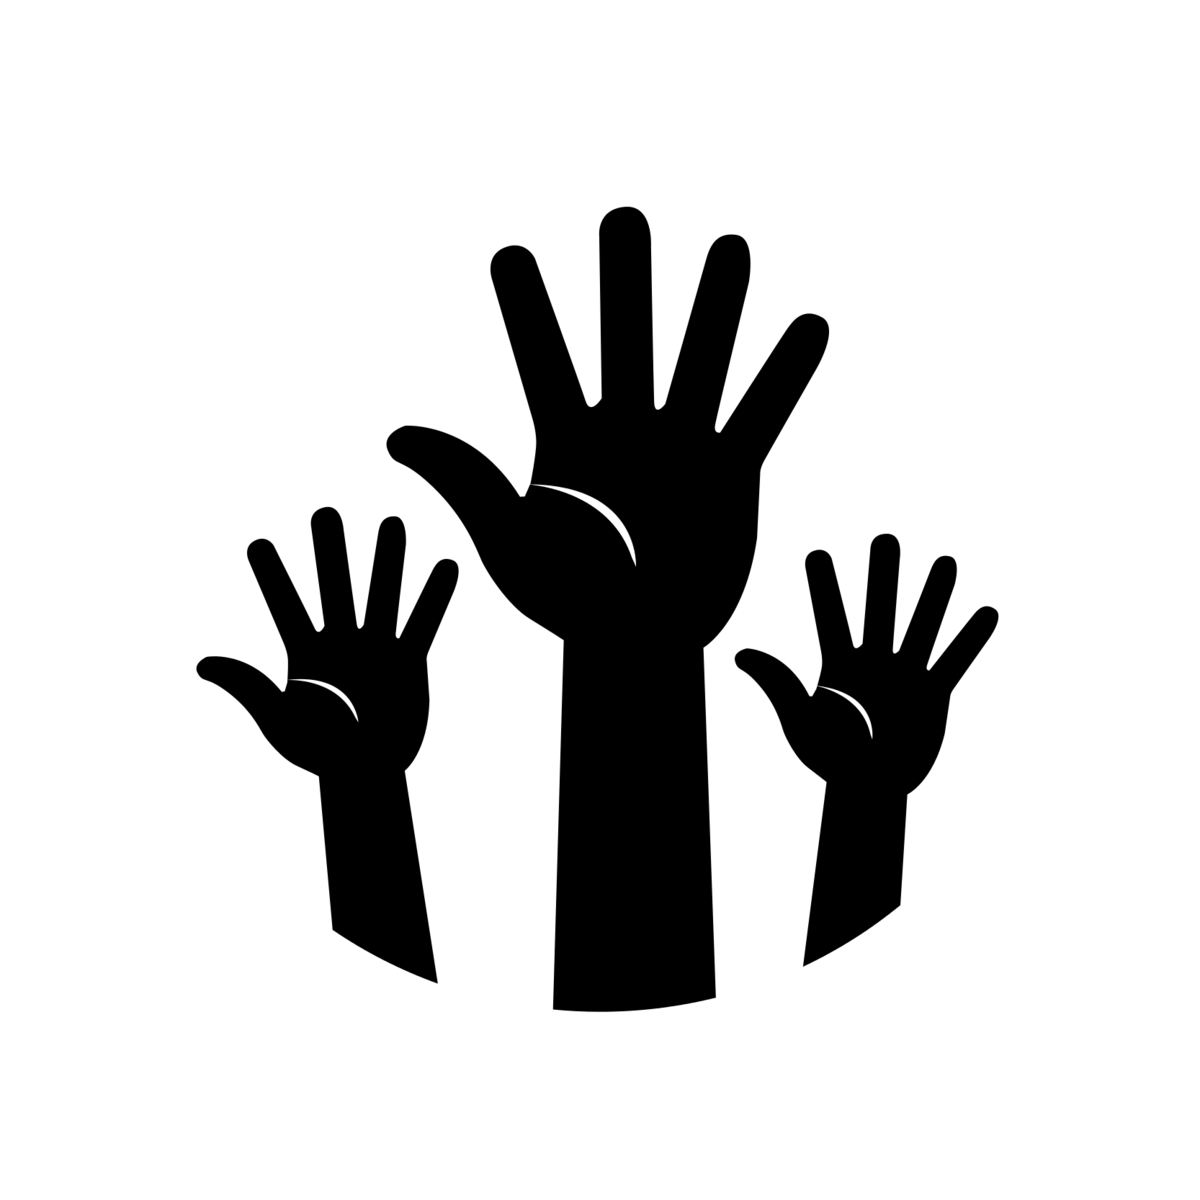
\includegraphics[scale=.03]{images/hands.png}
\alert{Design decisions?}:\\
\pause Probability parameter wp, evaluation function~$g$,\\ construction method of initial candidate

\end{frame}
%-----------------------------------------------------------------------
%----------------------------------------------------------------------
\begin{frame}[c]{Example: RII for SAT}

\centering

$F:= (\neg x_1 \vee x_2) 
		\wedge (\neg x_2 \vee x_1) 
		\wedge (\neg x_1 \vee \neg x_2 \vee \neg x_3) 
		\wedge ( x_1 \vee x_2) 
		\wedge (\neg x_4 \vee x_3) 
		\wedge(\neg x_5 \vee x_3) 
$

\bigskip

\begin{tabular}{lccccccc}
Step. & $x_1$ & $x_2$ & $x_3$ & $x_4$ & $x_5$ & Confl. Clauses & $g(s)$\\ 
\hline
1 Init & $\top$ & $\top$ & $\top$ & $\top$ & $\top$ & $C_3$ & $1$\\
\pause
2 Non-Impr. & $\top$ & $\top$ & $\bot$ & $\top$ & $\top$ & $C_5,C_6$ & $2$\\
\pause
3 Random & $\top$ & $\bot$ & $\bot$ & $\top$ & $\top$ & $C_1,C_4,C_5,C_6$ & $4$\\
\pause
4 Impr. & $\top$ & $\bot$ & $\bot$ & $\bot$ & $\top$ & $C_1,C_4,C_6$ & $3$\\
\pause
5 Impr. & $\top$ & $\bot$ & $\bot$ & $\bot$ & $\bot$ & $C_1,C_4$ & $2$\\
\pause
6 Random & $\top$ & $\bot$ & $\top$ & $\bot$ & $\bot$ & $C_1,C_4$ & $2$\\
\pause
7 Impr. & $\top$ & $\top$ & $\top$ & $\bot$ & $\bot$ & $C_3$ & $1$\\
\pause
8 Impr. & $\top$ & $\top$ & $\bot$ & $\bot$ & $\bot$ & $\checkmark$ & $0$\\
\end{tabular}

\end{frame}
%-----------------------------------------------------------------------
%-----------------------------------------------------------------------
\begin{frame}[c]{Variable Neighbourhood Descent (VND)}

\begin{block}{Idea}
Change (typically increase) the size of the neighbourhood relation over time. 
%I.e., $N_1,\ldots,N_{imax}$ is a set of neighbourhood relations, 
%typically ordered according to increasing size of the respective local neighbourhoods.
\end{block}

\begin{tabbing}
----\=----\=----\=----\=----\=----\=----\=----\=\kill
\> determine initial candidate solution $s$\\
\> $i$ := $1$\\
\> \pscRepeat\\
\> \vbar \> choose most improving neighbour $s'$ of $s$ in $N_i$\\[-0.55ex]
\> \vbar \> \pscIf\ $g(s') < g(s)$:\\[-0.55ex]
\> \vbar \> \> $s$ := $s'$\\[-0.55ex]
\> \vbar \> \> $i$ := $1$\\[-0.55ex]
\> \vbar \> \pscElse\ \\[-0.55ex]
\> \vendbar \> \> $i$ := $i+1$\\[-0.55ex]
\> \pscUntil\ $i > \param{k}$
\end{tabbing}

\pause

\vspace{-0.5cm}
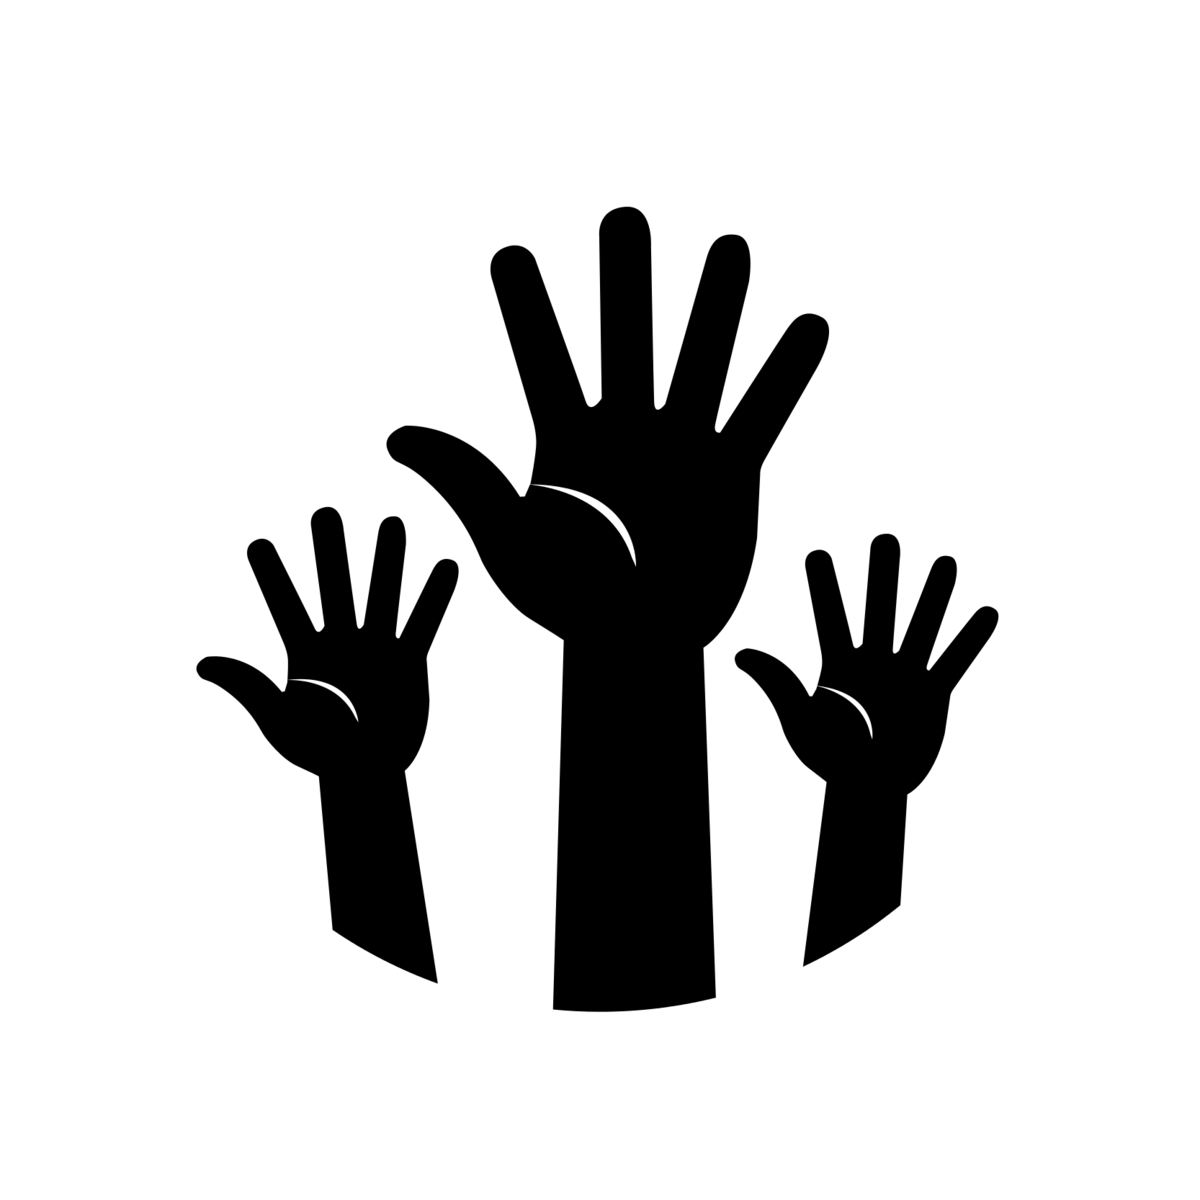
\includegraphics[scale=.03]{images/hands.png}
\alert{Design decisions?}:
\pause Design of increasing neighbourhood relation, evaluation function $g$,
construction method of initial candidate

\end{frame}
%-----------------------------------------------------------------------
%----------------------------------------------------------------------
\begin{frame}[c]{Example: VND for SAT}

\centering

$F:= (\neg x_1 \vee x_2) 
		\wedge (\neg x_2 \vee x_1) 
		\wedge (\neg x_1 \vee \neg x_2 \vee \neg x_3) 
		\wedge ( x_1 \vee x_2) 
		\wedge (\neg x_4 \vee x_3) 
		\wedge(\neg x_5 \vee x_3) 
$

\bigskip

\begin{tabular}{lccccccc}
Step. & $x_1$ & $x_2$ & $x_3$ & $x_4$ & $x_5$ & Confl. Clauses & $g(s)$\\ 
\hline
1 Init $i=1$ & $\top$ & $\top$ & $\top$ & $\top$ & $\top$ & $C_3$ & $1$\\
\pause
2 No Impr. $i=2$ & $\top$ & $\top$ & $\top$ & $\top$ & $\top$ & $C_3$ & $1$\\
\pause
3 No Impr. $i=3$ & $\top$ & $\top$ & $\top$ & $\top$ & $\top$ & $C_3$ & $1$\\
\pause
4 Impr. $i=1$ & $\top$ & $\top$ & $\bot$ & $\bot$ & $\bot$ & $\checkmark$ & $0$\\
\end{tabular}

\bigskip
\pause

Note: With large neighborhoods sizes, you have to check more potential solution candidates
to find the most improving neighbour. 

\end{frame}
%-----------------------------------------------------------------------
%-----------------------------------------------------------------------
\begin{frame}[c]{Simulated Annealing (SA)}

\begin{tabbing}
----\=----\=----\=----\=----\=----\=----\=----\=\kill
\> determine initial candidate solution $s$\\
\> set initial temperature $T$ according to annealing schedule\\
\> \pscWhile\ termination condition is not satisfied:\\
\> \vbar \> probabilistically choose a neighbour $s'$ of $s$ \\[-0.55ex]
\> \vbar \> \> using proposal mechanism\\[-0.55ex] 
\> \vbar \> \pscIf\ $s'$ satisfies probabilistic acceptance criterion ($p_{accept}(T,s,s')$):\\[-0.55ex]
\> \vbar \> \> $s$ := $s'$\\[-0.55ex]
\> \vend \> update $T$ according to annealing schedule
\end{tabbing}

\begin{equation}
p_{accept}(T,s,s')= \begin{cases}
					1 & \text{if } g(s') \leq g(s)\\
					\exp\left(\frac{g(s)-g(s')}{T}\right)  & \text{otherwise}
\end{cases}\nonumber
\end{equation}

\pause

Note: The annealing schedule may keep $T$ constant for a number of search steps.

\medskip
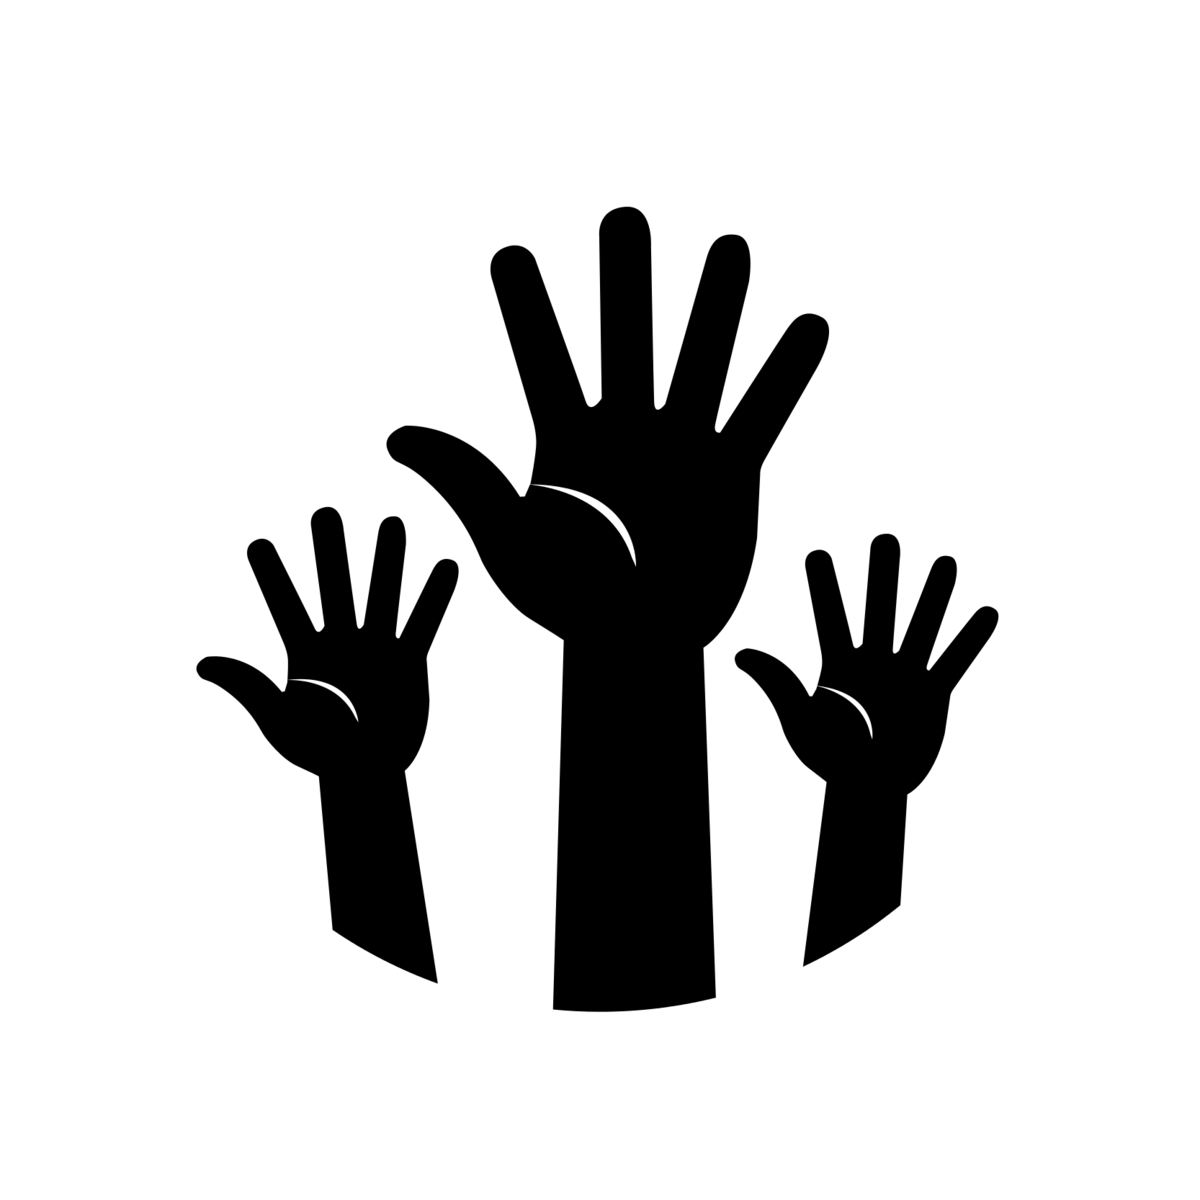
\includegraphics[scale=.01]{images/hands.png}
\alert{Design decisions?}:\\
\pause annealing schedule, proposal mechanism,\\ 
construction method of initial candidate

\end{frame}
%-----------------------------------------------------------------------
%-----------------------------------------------------------------------
\begin{frame}[c]{Tabu Search}

\begin{tabbing}
----\=----\=----\=----\=----\=----\=----\=----\=\kill
\> determine initial candidate solution $s$\\
\> \pscWhile\ \emph{termination criterion} is not satisfied:\\
\> \vbar \> determine set $N'$ of non-tabu neighbours of $s$\\[-0.55ex]
\> \vbar \> choose a best improving candidate solution $s'$ in $N'$\\[-0.55ex]
\> \vbar \\[-1.5ex]
\> \vbar \> update tabu attributes based on $s'$\\[-0.55ex]
\> \vend \> $s$ := $s'$ 
\end{tabbing}

Note: Tabu attributes are associated with solution components.

\medskip
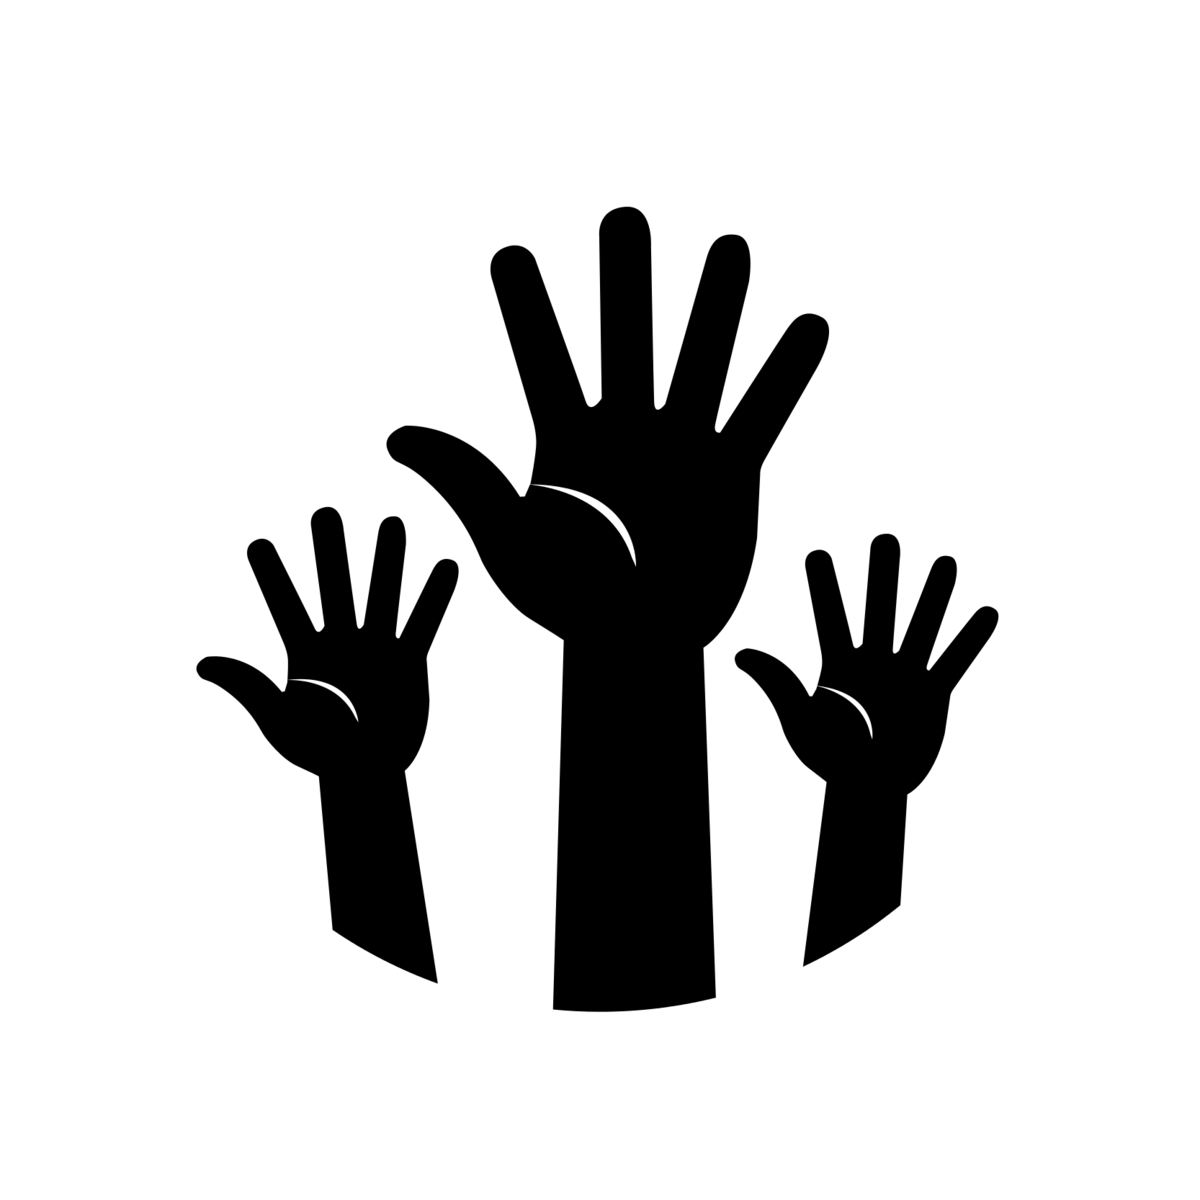
\includegraphics[scale=.03]{images/hands.png}
\alert{Design decisions?}:\\
\pause Design of tabu mechanism,\\ 
construction method of initial candidate

\end{frame}
%-----------------------------------------------------------------------
%----------------------------------------------------------------------
\begin{frame}[c]{Example: Tabu-Search for SAT}

\centering

$F:= (\neg x_1 \vee x_2) 
		\wedge (\neg x_2 \vee x_1) 
		\wedge (\neg x_1 \vee \neg x_2 \vee \neg x_3) 
		\wedge ( x_1 \vee x_2) 
		\wedge (\neg x_4 \vee x_3) 
		\wedge(\neg x_5 \vee x_3) 
$

\bigskip

\begin{tabular}{lccccccc}
Step. & $x_1$ & $x_2$ & $x_3$ & $x_4$ & $x_5$ & Confl. Clauses & Tabu\\ 
\hline
1 & $\bot$ & $\bot$ & $\bot$ & $\bot$ & $\bot$ & $C_4$ & $\emptyset$\\
\pause
2 & $\top$ & $\bot$ & $\bot$ & $\bot$ & $\bot$ & $C_1$ & $\{x_1\}$\\
\pause
3 & $\top$ & $\top$ & $\bot$ & $\bot$ & $\bot$ & $\checkmark$ & $\{x_1,x_2\}$\\
\end{tabular}


\end{frame}
%-----------------------------------------------------------------------
%-----------------------------------------------------------------------
\begin{frame}[c]{Dynamic Local Search (DLS)}

\begin{tabbing}
----\=----\=----\=----\=----\=----\=----\=----\=\kill
\> determine \emph{initial candidate solution $s$}\\
\> initialize penalties\\
\> \pscWhile\ \emph{termination criterion} is not satisfied:\\
\> \vbar \> compute modified evaluation function $g'$ from $g$ \\[-0.55ex]
\> \vbar \> \>                          based on penalties\\[-0.55ex]
\> \vbar \\[-1.5ex]
\> \vbar \> perform subsidiary local search on $s$ \\[-0.55ex]
\> \vbar \> \>        using evaluation function $g'$ \\[-0.55ex]
\> \vbar \\[-1.5ex]
\> \vend \> update penalties based on $s$
\end{tabbing}

Note: Penalties are associated with solution components; 
the subsidiary local search ends in a local optimum of $g'$.

\medskip
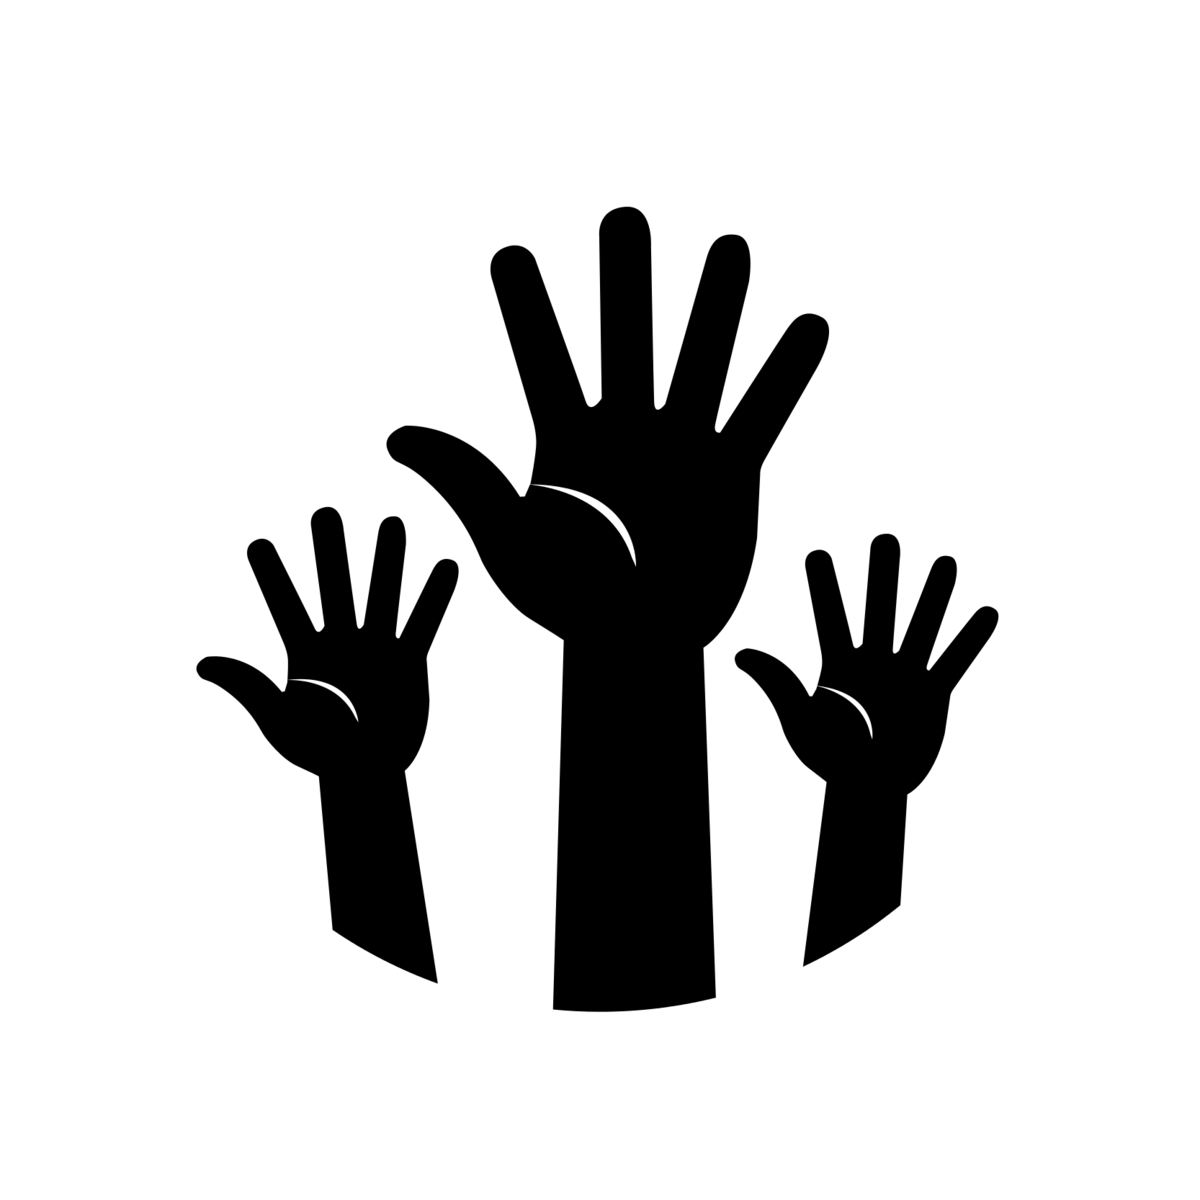
\includegraphics[scale=.03]{images/hands.png}
\alert{Design decisions?}:\\
\pause Design of $g$ (penalties), subsidiary local search \\ 
construction method of initial candidate

\end{frame}
%-----------------------------------------------------------------------
%-----------------------------------------------------------------------
\begin{frame}[c]{Iterated Local Search (ILS)}

\begin{tabbing}
----\=----\=----\=----\=----\=----\=----\=----\=\kill
\> determine initial candidate solution $s$\\
\> perform subsidiary local search on $s$\\
\> \pscWhile\ termination criterion is not satisfied:\\
\> \vbar \> $r$ := $s$\\[-0.55ex]
\> \vbar \> perform perturbation on $s$ \hspace{0.8em} \texttt{\% n random steps in neighbourhood}\\[-0.55ex]
\> \vbar \> perform subsidiary local search on $s$\\[-0.55ex]
\> \vbar \\[-1.5ex]
\> \vbar\> based on acceptance criterion, \\[-0.55ex]
\> \vend \> \> keep $s$ or revert to $s:=r$
\end{tabbing}

Note: The search history may additionally influence the perturbation phase
and the acceptance criterion.

\medskip
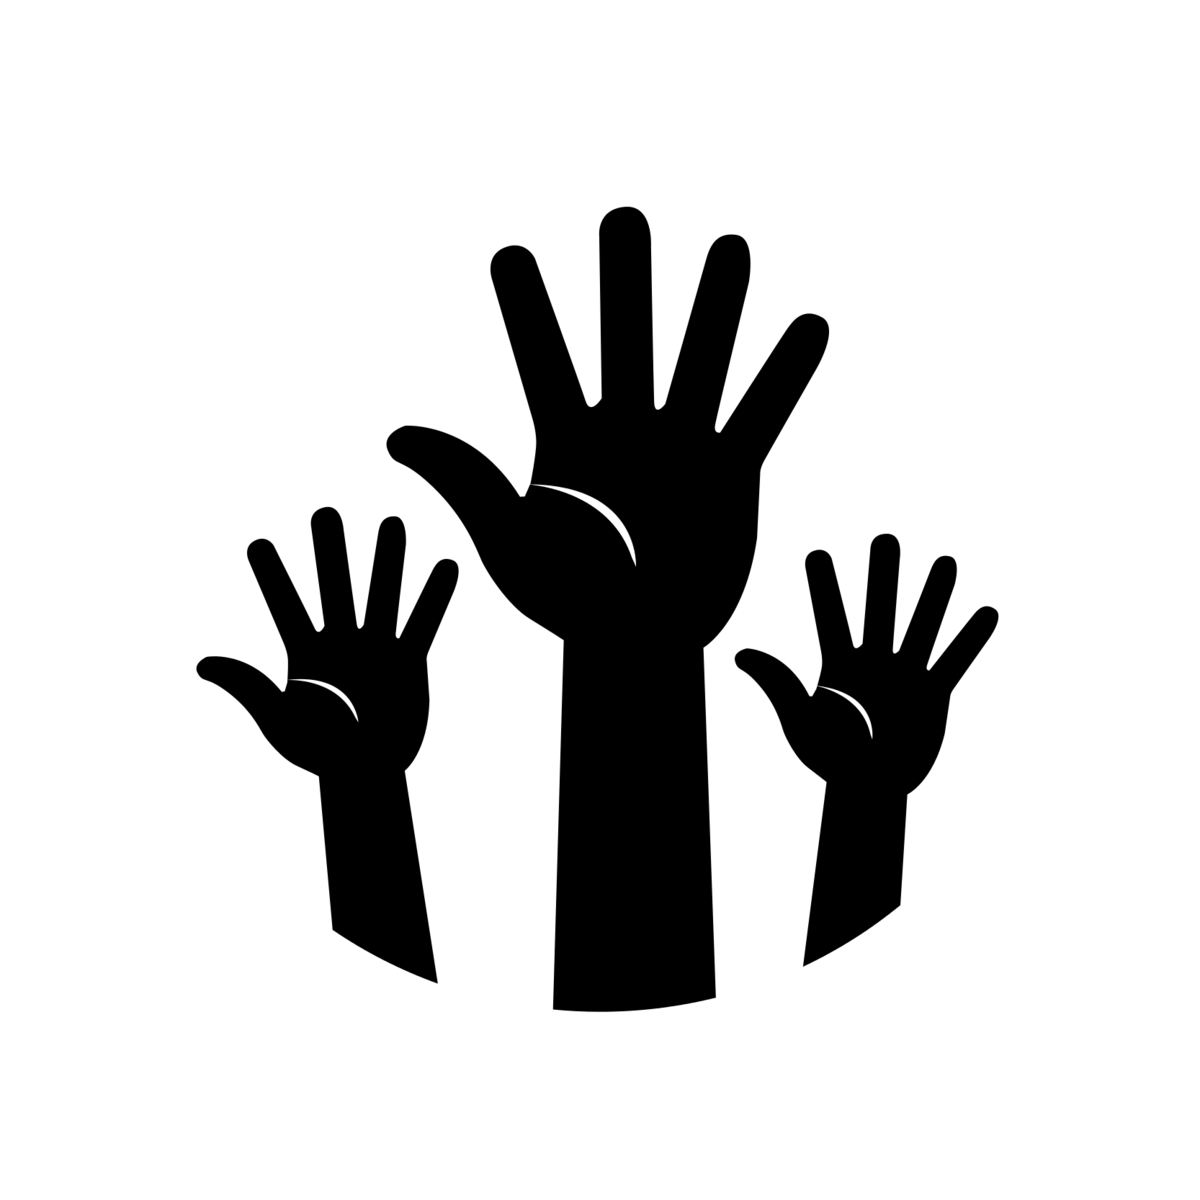
\includegraphics[scale=.03]{images/hands.png}
\alert{Design decisions?}:\\
\pause Strength of perturbation, subsidiary local search, acceptance criterion\\ 
construction method of initial candidate

\end{frame}
%-----------------------------------------------------------------------
% %-----------------------------------------------------------------------
% \begin{frame}[c]{Greedy Randomized ``Adaptive'' Search Procedure (GRASP)}
% 
% \begin{tabbing}
% ----\=----\=----\=----\=----\=----\=----\=----\=\kill
% \> \pscWhile\ \emph{termination criterion} is not satisfied:\\
% \> \vbar \> generate candidate solution $s$ using \\[-0.55ex]
% \> \vbar \> \>  subsidiary greedy randomized constructive search\\[-0.55ex]
% \> \vbar \\[-1.5ex]
% \> \vend \> perform subsidiary local search on $s$
% \end{tabbing}
% 
% Note: Randomization in \emph{constructive search} ensures that a large number
%         of good starting points for \emph{subsidiary local search} is obtained.
% 
% \begin{block}{Constructive Search:}
% \begin{enumerate}
%   \item Start with an empty candidate solution
%   \item Repeatedly, extend the current solution until a complete solution is constructed
%   \item Use heuristics to extend in such a way that the final solution is a good one
% \end{enumerate}
% \end{block}
% 
% \end{frame}
% %-----------------------------------------------------------------------
%----------------------------------------------------------------------
\begin{frame}[c]{}

\centering
\huge
Solving Combinatorial Problems:\\
Evolutionary Algorithms

\end{frame}
%----------------------------------------------------------------------
%----------------------------------------------------------------------
\begin{frame}[c]{Population-based Algorithms}

\begin{block}{Population:}
\begin{itemize}
  \item Set of candidate solutions $=$ population of individuals
  \item Evolve population over time such that ``fitness'' of population improves
  \item Fitness: can either correspond to objective function $f$ or evaluation function $g$
\end{itemize}
\end{block}

\pause

\begin{block}{Comparison to SLS:}
\begin{itemize}
  \item SLS typically converges faster to good intermediate solution
  \item Population-based algorithms are less often trapped in local optima
  \item Population-based algorithms are even easier to parallelize
  \begin{itemize}
    \item evaluate $f$ (or $g$) of each individual in parallel
  \end{itemize}
\end{itemize}
\end{block}

\end{frame}
%----------------------------------------------------------------------
%----------------------------------------------------------------------
\begin{frame}[c]{Genetic Algorithms}

\begin{center} 
	\includegraphics[width=0.50\textwidth]{images/ea.png}  
\end{center}
{\tiny Source: ``Introduction to Evoluationary Computing'' by Eiben and Smith }

\bigskip
\pause

\begin{block}{Central Idea}
A solution candidate can be described by its solution components\\ (also called genes),
for example, variable assignment of each variable.
\end{block}

\bigskip
\pause
Note: Each step of a genetic algorithm implies new design choices!

\end{frame}
%----------------------------------------------------------------------
%----------------------------------------------------------------------
\begin{frame}[c]{Genetic Algorithms: Mutation}

\begin{block}{Mutation:}
\begin{itemize}
  \item With probability $p$, mutate a given individual.
  \item Mutation: perturbate a solution candidate 
\end{itemize}
\end{block}

\pause
\bigskip

\centering
\begin{tabular}{lccccc}
& $x_1$ & $x_2$ & $x_3$ & $x_4$ & $x_5$\\
\hline
Parent & $\bot$ & $\bot$ & $\bot$ & $\bot$ & $\bot$ \\
\pause
Offspring & $\bot$ & $\top$ & $\bot$ & $\bot$ & $\bot$ \\
\end{tabular}

\pause
\medskip
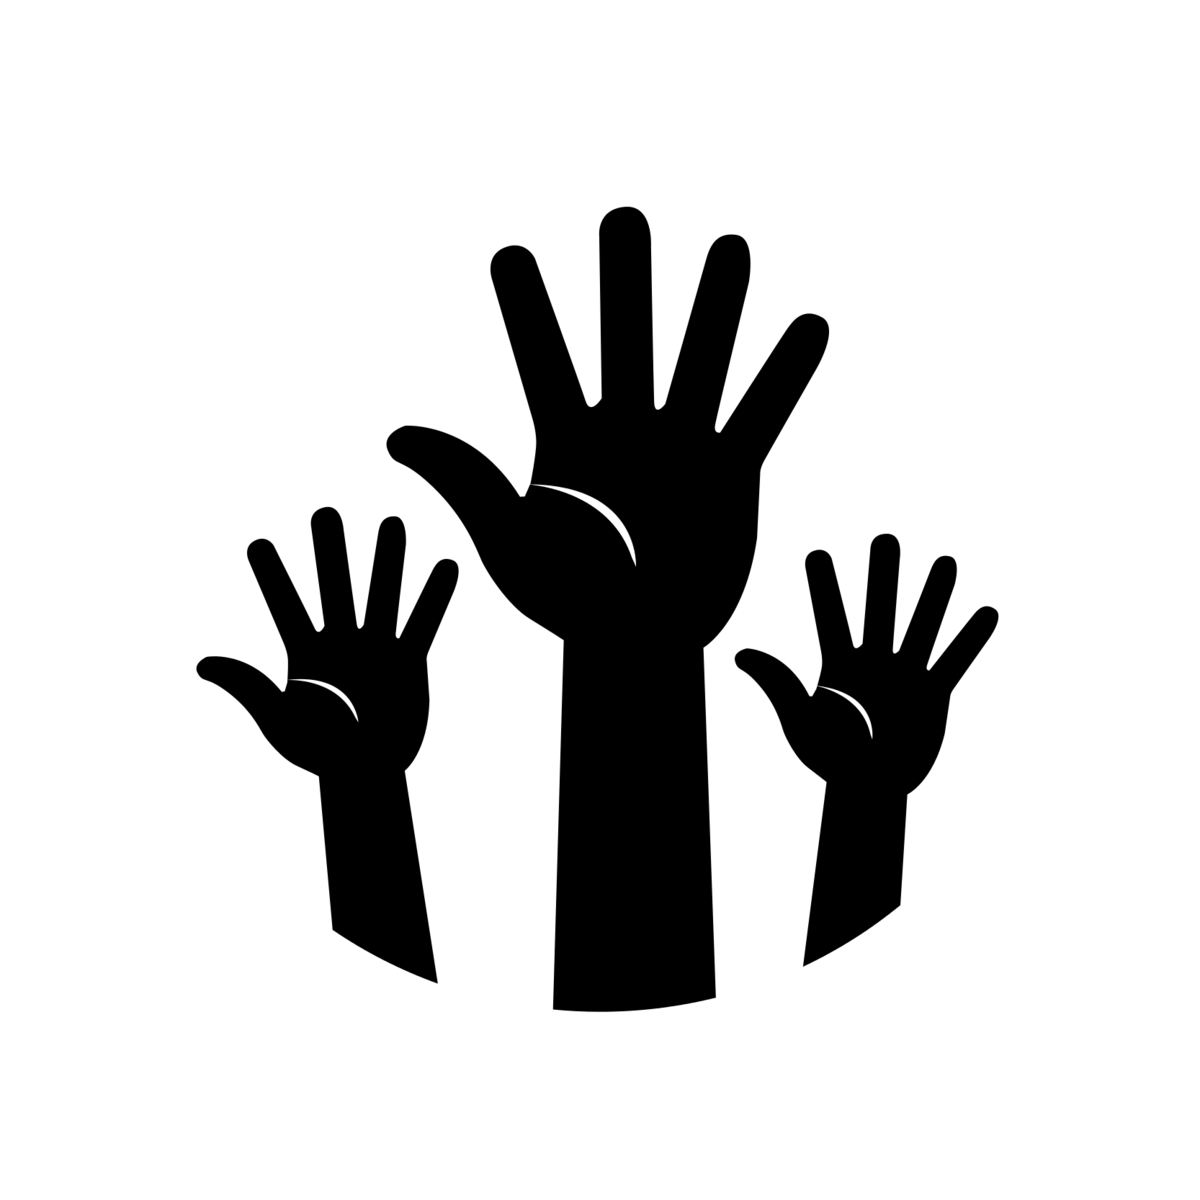
\includegraphics[scale=.03]{images/hands.png}
\alert{Design decisions?}:\\
\pause Strength of mutation, probability of mutation,\\
mutation operator (e.g., bit-wise or swaps)


\end{frame}
%----------------------------------------------------------------------
%----------------------------------------------------------------------
\begin{frame}[c]{Genetic Algorithms: Recombination}

\begin{block}{Mutation:}
\begin{itemize}
  \item Selection of two parents
  \item Recombine them to obtain off-spring
\end{itemize}
\end{block}

\pause
\bigskip

\centering
\begin{tabular}{lcccccc}
& $x_1$ & $x_2$ & & $x_3$ & $x_4$ & $x_5$\\
\hline
Parent 1 & $\bot$ & $\bot$ & & $\bot$ & $\bot$ & $\bot$ \\
Parent 2 & $\top$ & $\bot$ & & $\top$ & $\bot$ & $\top$ \\
\pause
Offspring & $\bot$ & $\bot$ & $\mid$ & $\top$ & $\bot$ & $\top$ \\
\end{tabular}

\pause
\medskip
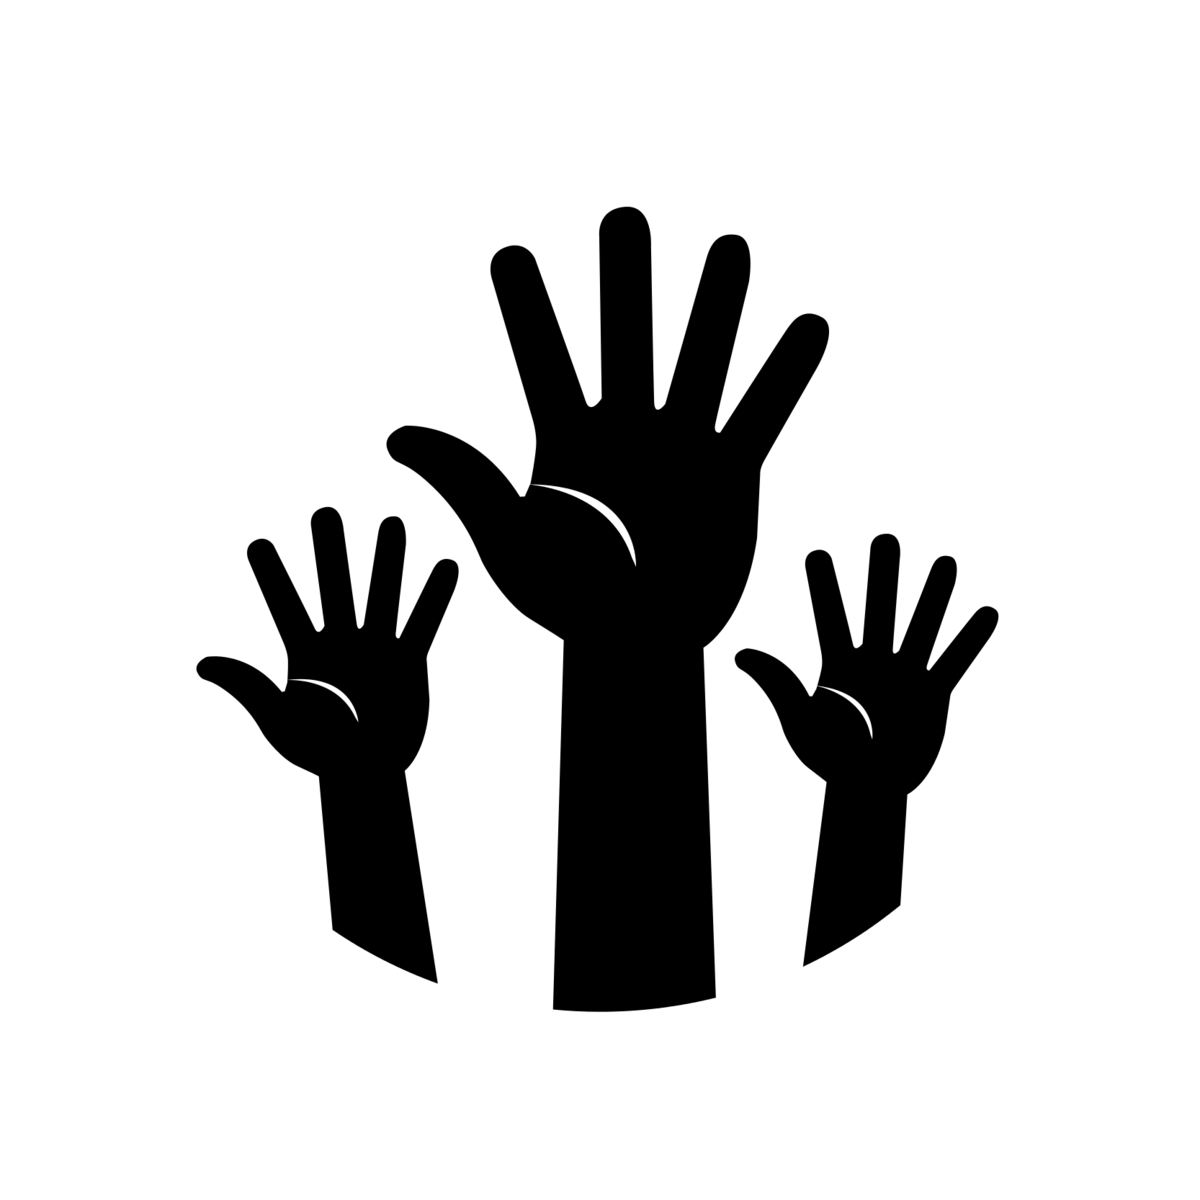
\includegraphics[scale=.03]{images/hands.png}
\alert{Design decisions?}:\\
\pause recombination (e.g., how many split points), parent selection

\end{frame}
%----------------------------------------------------------------------
%----------------------------------------------------------------------
\begin{frame}[c]{Genetic Algorithms: Selection and Evaluation}

\begin{block}{Design decisions:}
\begin{itemize}
  \item Evaluate all individuals and select best ones (also called tournament)
  \begin{itemize}
    \item how many to select?
  \end{itemize}
  \pause
  \item Evaluate only half of population (competitive half) and use selection on these
  \begin{itemize}
    \item Stronger diversification; less risk of local optima
    \item How to split population?
  \end{itemize}
  \pause
  \item Remove individuals only if they have certain age\\ (survived $n$ iterations)
  \begin{itemize}
    \item Stronger diversification; slower convergence to local optima
    \item $n$?
  \end{itemize}
  \pause
  \item \ldots
\end{itemize}
\end{block}

$\leadsto$ Again many design choices

\end{frame}
%----------------------------------------------------------------------
%----------------------------------------------------------------------
\begin{frame}[c]{}

\centering
\huge
Machine Learning Algorithms

\end{frame}
%----------------------------------------------------------------------
\begin{frame}[c]{k-Nearest Neighbor}

\includegraphics[width=0.8\textwidth]{images/kNN}

\end{frame}
%-----------------------------------------------------------------------
%----------------------------------------------------------------------
\begin{frame}[c]{k-Nearest Neighbor}

\begin{block}{Training}
Nothing to do (na\"ive implementation)
\end{block}

\bigskip

\begin{block}{Predict (Classification)}
\begin{enumerate}
  \item Determine the $k$ nearest neighbors in feature space $\mathcal{X}$
  \item Return the most often used class of the neighbors
\end{enumerate}
\end{block}

\pause
\begin{block}{Predict (Regression)}
\begin{enumerate}
  \item Determine the $k$ nearest neighbors in feature space $\mathcal{X}$
  \item Return the average value of the neighbors
\end{enumerate}
\end{block}

\end{frame}
%-----------------------------------------------------------------------
%----------------------------------------------------------------------
\begin{frame}[c]{Design Decisions in k-Nearest Neighbor}

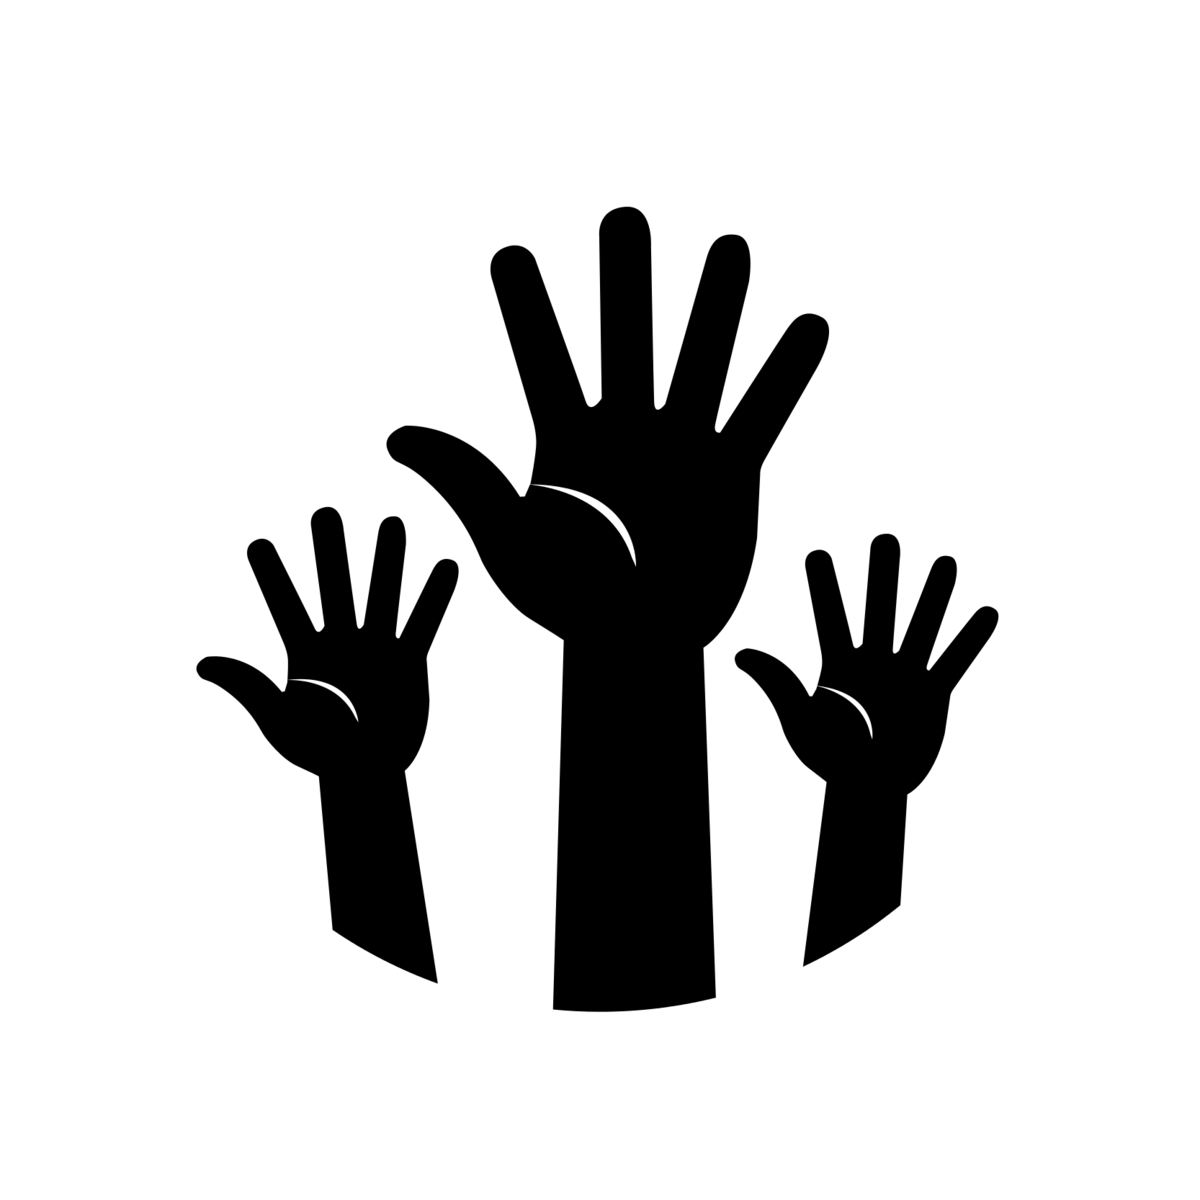
\includegraphics[scale=0.05]{images/hands}
\pause

\begin{itemize}
  \item $k$: size of neighborhood
  \item distance metric (e.g., euclidean or manhattan)
  \item (search algorithm to determine neighbors)
\end{itemize}

\end{frame}
%-----------------------------------------------------------------------
%----------------------------------------------------------------------
\begin{frame}[c]{Tuning of $k$}

\centering
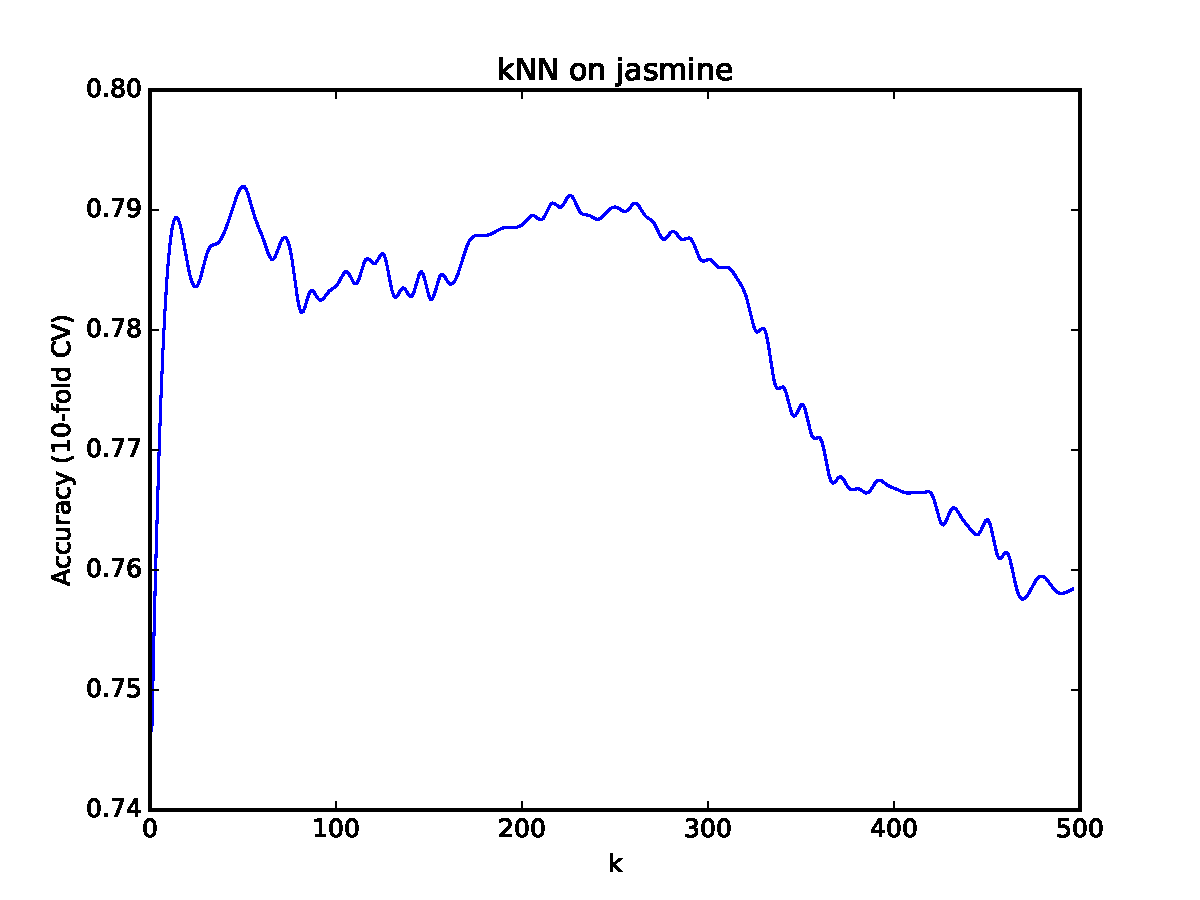
\includegraphics[scale=.5]{images/kNN-jasmine}

\end{frame}
%-----------------------------------------------------------------------
%----------------------------------------------------------------------
\begin{frame}[c]{Decision Trees}

\begin{itemize}
  \item One of the most basic ML algorithms
\end{itemize}

\centering
\includegraphics[width=0.7\textwidth]{images/iris_tree}

(source: scikit-learn)
\end{frame}
%-----------------------------------------------------------------------
%----------------------------------------------------------------------
\begin{frame}[c]{Regression Trees}

\begin{itemize}
  \item Same kind of splits, but with continuous values in leafs\\ (instead of classes)
\end{itemize}

\centering
\includegraphics[width=0.7\textwidth]{images/regression_tree_pred.png}

(source: scikit-learn)
\end{frame}
%-----------------------------------------------------------------------
%----------------------------------------------------------------------
\begin{frame}[c]{Build Decision Tree}

\begin{algorithm}[H]
\Input{$D = \{(\vec{x}^{(i)}, y^{(i)})\}_{i\in \{1\ldots|D|\}}$, attributes A}
\BlankLine
\If{all $y^{(i)}$ have the same class} {
	  \Return{Leaf with class $y$}
}
\pause
\If{attributes $=$ $\emptyset$}{
	\Return{Leaf with most frequent class}
}
\pause
let $a \in A$ be the \emph{best attribute};\\ 
\For{all values $v$ of $a$ in $D$}{
	Create edge with  constraint $a = v$;\\
	BuildTree($\{ (\vec{x}^{(i)}, y^{(i)}) \in D | \vec{x}^{(i)}.a = v\}$, $A - \{a\}$);
}
	
\Return{current node}
\caption{\texttt{BuildTree()} with categorical attributes}
\end{algorithm}

\footnotesize
\pause
Note: ``best attribute'' determined by a loss function\\ (e.g., RMSE for regression problems)\\
\pause
Note(2): loss function can be weighted by sample weights\\ (e.g., can be used for cost-sensitive algorithm selection)

\end{frame}
%-----------------------------------------------------------------------
%----------------------------------------------------------------------
\begin{frame}[c]{Design Decisions in Decision/Regression Trees?}

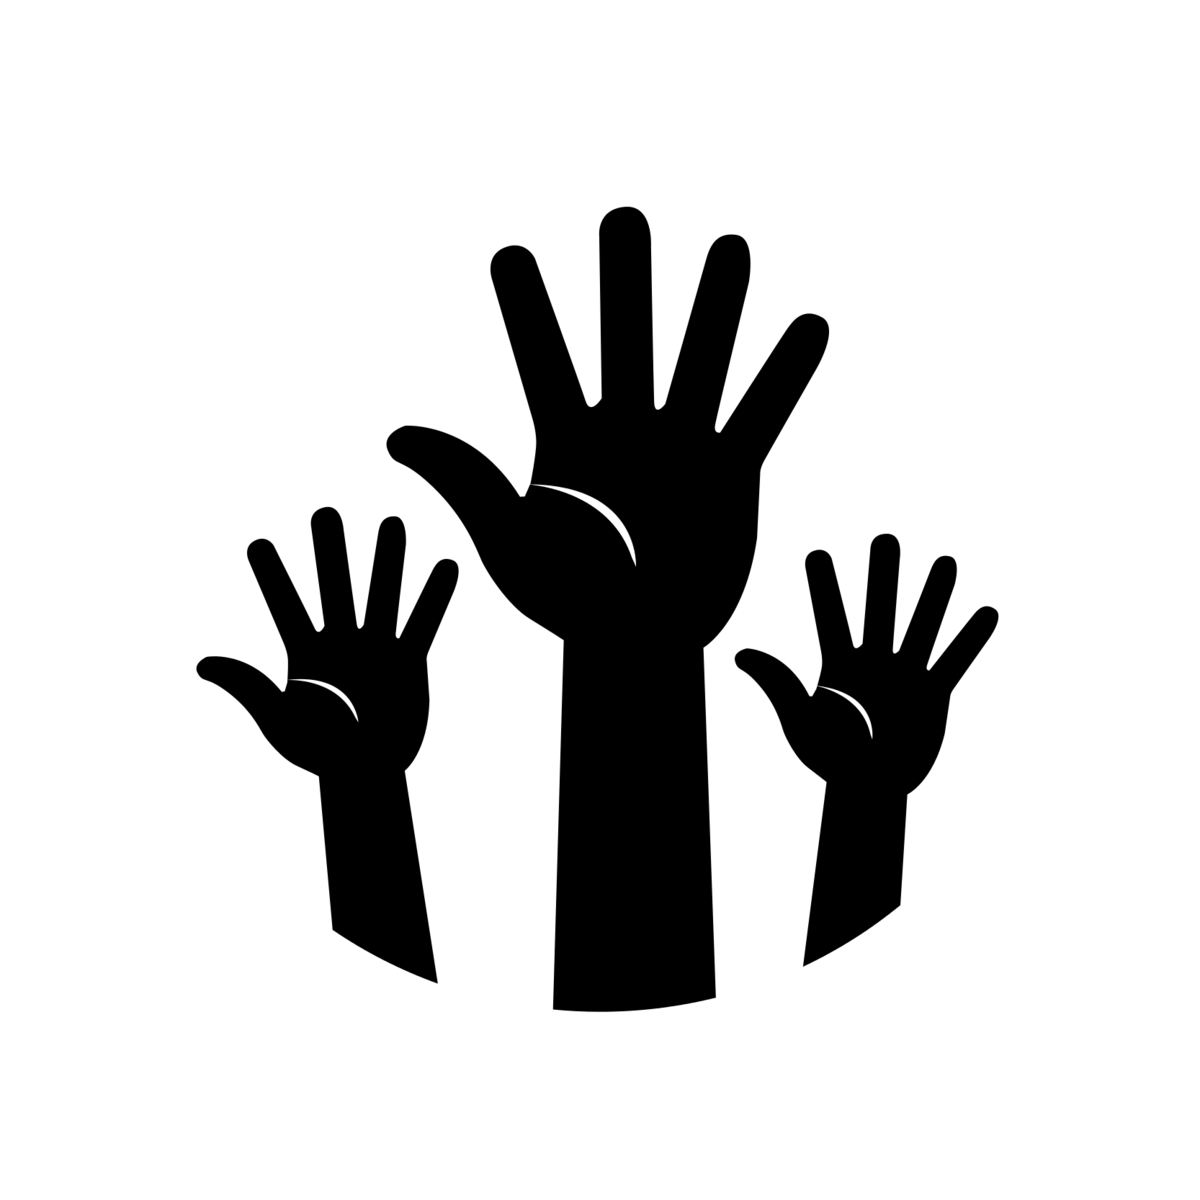
\includegraphics[scale=0.05]{images/hands}
\pause

\begin{itemize}
  \item splitting criterion (Gini, entropy, mse, \ldots)
  \item max depth
  \item min samples to split
  \item min samples in leaf
  \item max leaf nodes
  \item minimal impurity 
\end{itemize}

\end{frame}
%-----------------------------------------------------------------------
%----------------------------------------------------------------------
\begin{frame}[c]{Random Forest (Regression)}

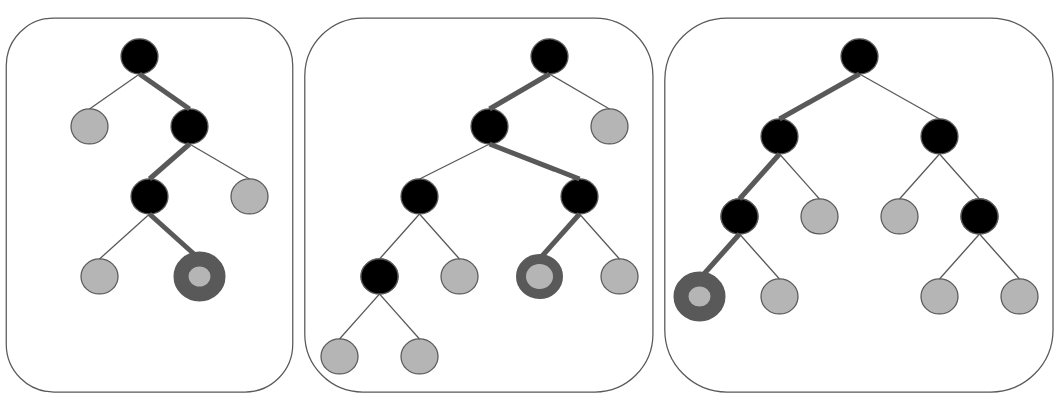
\includegraphics[width=0.9\textwidth]{images/random_forest_pic}

\begin{itemize}
  \item train several trees
  \item subsample observations and features in each tree
  \pause
  \item Prediction: average across tree predictions
  \pause
  \item Uncertainty: stdev across tree predictions
\end{itemize}

\end{frame}
%-----------------------------------------------------------------------
%----------------------------------------------------------------------
\begin{frame}[c]{Design Decisions in Random Forest}

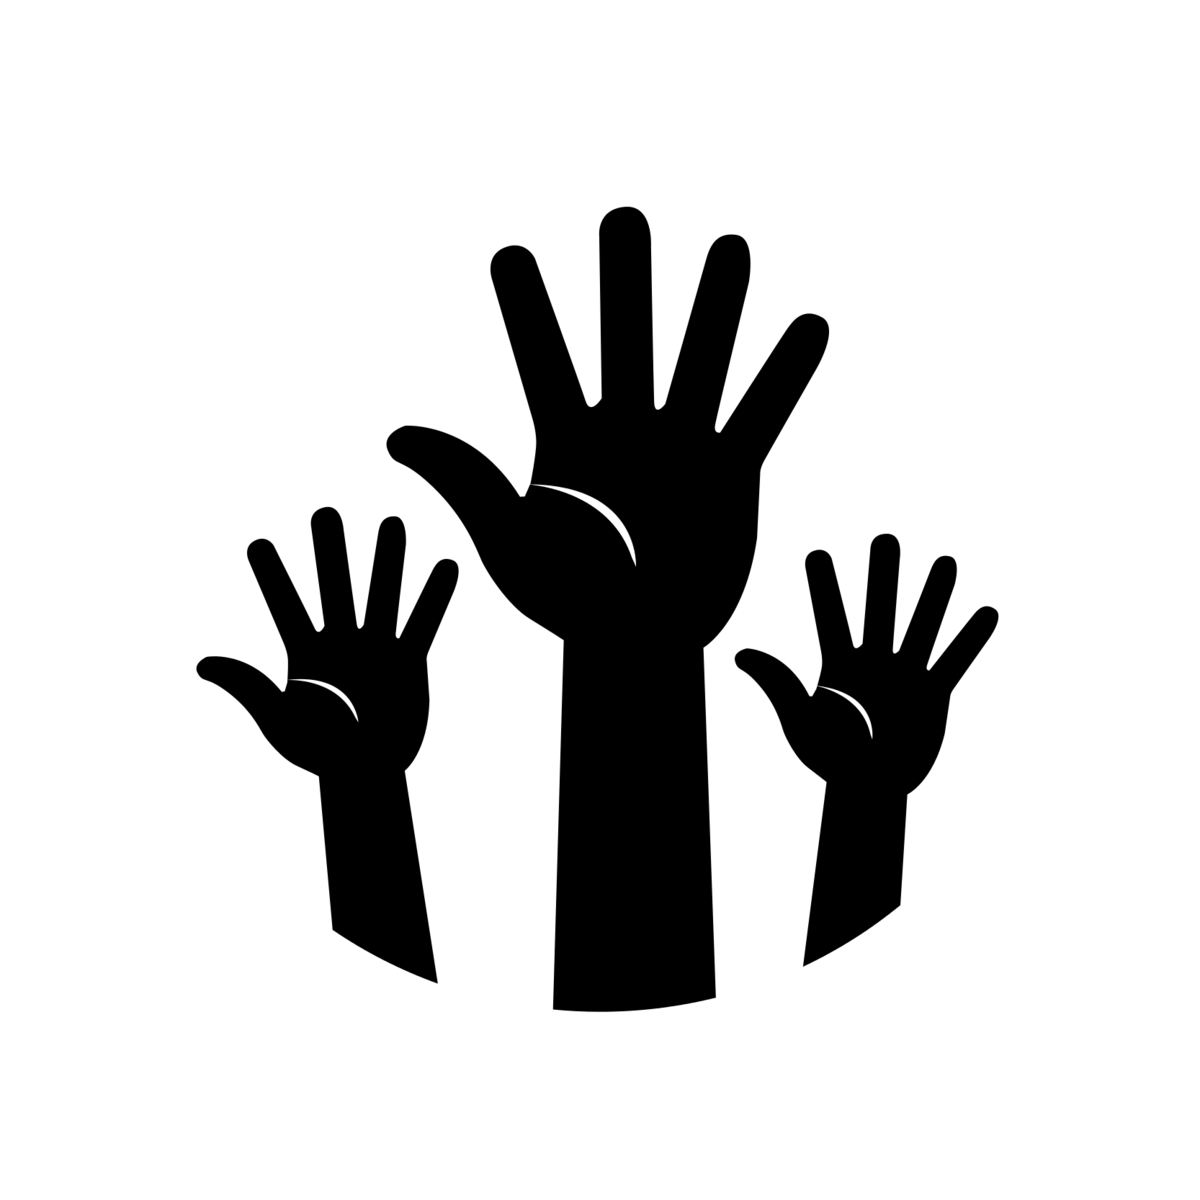
\includegraphics[scale=0.05]{images/hands}
\pause

\begin{itemize}
  \item same as for decision/regression trees
  \item aggregation strategy
  \item use of bootstrapping for sampling observations
  \item subsampling strength of observations
  \item subsampling strength of features
\end{itemize}

\end{frame}
%-----------------------------------------------------------------------
%----------------------------------------------------------------------
\begin{frame}[c]{Deep Neural Network}

\begin{itemize}
  \item most famous ML algorithm these days
  \item each layer of neurons applies a linear transformation\\
   and a non-linear activation function  $g$ on top 
\end{itemize}

\begin{eqnarray}
z_i = \vec{W}_i\vec{h_i} + \vec{b}_i\\
h_{i+1} = g(z_i)
\end{eqnarray}



\centering
\includegraphics[width=0.8\textwidth]{images/dnn_pic}

\begin{itemize}
  \item last neuron can use a softmax for $g$ (classification problem)
\end{itemize}

\end{frame}
%-----------------------------------------------------------------------
%----------------------------------------------------------------------
\begin{frame}[c]{Training of Deep Neural Network}

\begin{block}{Loss function}
\begin{itemize}
  \item Optimal weights are defined by a loss function
  \item Example of squared error (for regression)
\end{itemize}

\begin{equation}
L(\vec{W}) = \frac{1}{2} \sum_{n=1}^N \left( \hat{y}(\vec{x}_n, \vec{W}) - y_n  \right)
\end{equation}
\end{block}

\pause

\begin{block}{Optimization of loss function}
\begin{itemize}
  \item typically, we use stochastic gradient descent (SGD)\\
  (or variants of SGD)
  \item chain rule over layers to use it efficiently for deep learning
  \item Iteratively update weights (on batches of samples):
\end{itemize}

\begin{equation}
\vec{W} = \vec{W} - \eta \nabla L(\vec{W})
\end{equation}

\end{block}

\end{frame}
%-----------------------------------------------------------------------
%----------------------------------------------------------------------
\begin{frame}[c]{Design Decisions in Deep Neural Network}

\includegraphics[scale=0.05]{images/hands}

\end{frame}
%-----------------------------------------------------------------------
\begin{frame}[c]{Summary: Learning Goals}

What have we learned today?

\begin{enumerate}
  \item Recap: Optimization algorithms
  \begin{itemize}
    \item Stochastic local search (SLS)
    \item Evolutionary algorithms
  \end{itemize}
  \item Recap: Machine learning algorithms
  \begin{itemize}
    \item kNN, tree-based algorithms, neural networks
  \end{itemize}
  \item What are typical decisions in algorithm design?
\end{enumerate}

\end{frame}
%-----------------------------------------------------------------------
%\newcommand{\answer}[1]{\textcolor{black}{#1}}

\newcommand{\rt}{T}
\newcommand{\RT}{T}
\newcommand{\sq}{Q}
\newcommand{\SQ}{Q}
\newcommand{\sr}{r}
%----------------------------------------------------------------------
\begin{frame}[c]{Where are we? The big picture}

\begin{itemize}
\item Algorithm Selection
  \begin{itemize}
    \item Portfolios
    \item Algorithm selection (for runtime)
  \end{itemize}
  \item Design decisions:\\ Local Search + Evo. Algorithms + Machine Learning 
  \item[$\to$] Empirical evaluation
  \item AAD for ML
  \begin{itemize}
    \item Hyperparameter optimization and Bayesian optimization 
    \item Neural architecture search (lecture given by Prof. Hutter)
  \end{itemize}
  \item Algorithm configuration 
  \begin{itemize}
    \item Basics 
    \item State of the art 
    \item Best practices 
  \end{itemize}
  \item Combinations of algorithm selection and configurations
  \item Algorithm control 
  \item Algorithm analysis 
  \item Project announcement and questions for exam 
\end{itemize}

\end{frame}
%----------------------------------------------------------------------
%----------------------------------------------------------------------
\begin{frame}[c]{}

\centering
\huge
Empirical Evaluation

\end{frame}
%----------------------------------------------------------------------
%----------------------------------------------------------------------
\begin{frame}[c]{Motivation}

\begin{itemize}
  \item Ultimately, we'll discuss how to \alert{improve empirical performance}
  \bigskip
  \item We first need a solid understanding of\\how to \alert{measure empirical performance}
  \begin{itemize}
    \item Comparing algorithms or parameter configurations
    \begin{itemize}
      \item[$\to$] Focus today!
    \end{itemize}
    \item Algorithm configurations\\ (empirical performance of parameter configurations)
    \item Data collection to train algorithm selection models 
  \end{itemize}  
\end{itemize}

\end{frame}
%-----------------------------------------------------------------------
%----------------------------------------------------------------------
\begin{frame}[c]{Learning Goals}

After this lecture, you will be able to \ldots

\begin{itemize}
  \item explain how computer science (CS) differs from other empirical sciences
  \item compare performances of algorithms by using \alert{visualization techniques}
  \begin{itemize}
    \item tabular comparison
    \item runtime distributions
    \item scatter plots
    \item box plots
  \end{itemize}
  \item explain how \alert{statistical tests} can be used 
  \item \alert{apply all these techniques} to algorithms\\ from hard combinatorial optimizations and machine learning
\end{itemize}

\pause

\alert{Note:} We assume today that we already measured the performance values.\\
In a later session, we will discuss pitfalls and best practices concerning the measurement itself.

\end{frame}
%-----------------------------------------------------------------------

%----------------------------------------------------------------------
\begin{frame}{How CS differs from other empirical sciences}

\begin{itemize}
	\item We have a complete and precise \alert{mathematical description}\\of the object under study
	\smallskip
	
	\item We have complete and precise \alert{control} of the object under study\\ 
  (and to some degree also the experimental environment)
	\begin{itemize}
	  	\item as a result, experiments can be \alert{reproduced perfectly}
	  	\pause
	 	\item what do we need for experiments to be reproducible? 
	  	\only<2-2>{\includegraphics[height=1.5em]{images/hands}
	  	}
	  	\only<3->{
		  \begin{itemize}
		  	\item  \answer{Code \& dependencies, inputs, environment ($\rightarrow$ VM \& cloud)}
		  \end{itemize}
	  	\pause
		}
	\end{itemize}
  \medskip
	  	\pause
	
%\only<4->{
  \item We often have quite \alert{cheap} experiments
  \begin{itemize}
  	\item price for computers is monotonically decreasing
  	\item often maximal runtimes of 1h; exception: deep learning (up to a week)
  	\item compare e.g., experimental physics: 1 week of beam time per year % Still different from observing new species in the field for half a year / 
  \end{itemize}
  \smallskip
  \pause
%}
%\only<5->{
  \item We can conduct and analyze experiments fully \alert{automatically} 
  \begin{itemize}
    \item we can gather large amounts of data quickly (e.g., 100 repetitions)
  	\item but: don't confuse statistical significance and relevance
  \end{itemize}
%}	
\end{itemize}

\end{frame}
%-----------------------------------------------------------------------
%----------------------------------------------------------------------
\begin{frame}[c]{Outliers are quite different in computer experiments}

Is the following statement correct? \includegraphics[height=1.5em]{images/hands}

``As usual in other empirical sciences, we (in CS) should take care to \alert{detect and remove outliers} before further analysis.''

\pause
\bigskip

\begin{block}{Outliers in CS}
\begin{itemize}
  \item outliers should be investigated closely -- why is there an outlier?
  \item outliers are (hopefully) reproducible -- narrow down their reason!
  \pause
  \begin{itemize}
    \item \textbf{Algorithm:} When characterizing runtimes of a randomized algorithm on a single instance of a hard combinatorial problem, \alert{outliers with large values can indicate deep local optima}
    \pause
    \item \textbf{Environment:} Outliers with large runtimes can indicate a \alert{problem with the runtime environment} (e.g., file system or network issues)
    \pause
    \item \textbf{Instances:}  When characterizing runtimes across a distribution of instances, outliers with small values can indicate trivial instances.
  \end{itemize}
\end{itemize}
\end{block}

\end{frame}
%-----------------------------------------------------------------------
%----------------------------------------------------------------------
\begin{frame}[c]{Application scenarios and evaluation criteria}

Evaluation criteria for algorithms depend on the application context:

\bigskip

\begin{itemize}
\item {\bf Type 1:} \alert{No time limits} 
	\begin{itemize}
		\item Algorithm can be run until a (optimal) solution is found\\(off-line computations, \eg{}, configuration of production facility)
        
        \medskip
        \item[$\leadsto$] evaluation criterion (to minimize): \alert{expected run-time}
	\end{itemize}
        
\pause
\bigskip

\item {\bf Type 2:} \alert{Hard time limit $t_{max}$} 
	\begin{itemize}
		\item Solutions found later than $t_{max}$ are useless\\
        (real-time environments with strict deadlines,\\ \eg{}, dynamic task scheduling or on-line robot control)
        
        \medskip
        \item[$\leadsto$] evaluation criterion (to maximize): \alert{solution probability at time $t_{max}$}
	\end{itemize}
\end{itemize}

\end{frame}
%-----------------------------------------------------------------------

%----------------------------------------------------------------------
\begin{frame}[c]{Application scenarios and evaluation criteria}


In many real applications, utility of solutions depends in more complex ways on time required for finding them:

\medskip

\begin{itemize}
\item {\bf Type 3:}
        Characterized by \alert{utility function $U: \Reals^+ \mapsto [0,1]$},
        where $U(t)$ = utility of solution found at time $t$.
        
  \pause
  \bigskip

	\begin{itemize}
 	  \item \emph{Example:} Direct benefit $u_0$ of solution is invariant over time, \\
        but compute time costs a fixed rate: $U(t) := u_0 - c \cdot t$
        
        \pause
        \bigskip

       \item \alert{Decision-theoretic evaluation criterion} (to maximize): \\
                {utility-weighted solution probability} $U(t) \cdot P_s(\rt \leq t)$       \\
                $\leadsto$ requires detailed knowledge of $P_s(\rt \leq t)$ for arbitrary $t$
	\end{itemize}
        
\end{itemize}

\pause
\bigskip

{\small{Note: Type 3 is a generalization of Types 1 and 2.}}% We'll show that in an exercise.}}
%\note{Let students write down $U(t)$ for type 1 and 2 scenarios.}


\end{frame}
%-----------------------------------------------------------------------



%%%%%%%%%%%%%%%%%%%%%%%%%%%%%%%%%%%%%%%%%%%%%%%%%%%%%%%%%%%%%%%%%%%%%%%%%%%%%%5555
%\section{Runtime Distributions (RTDs)}
%%%%%%%%%%%%%%%%%%%%%%%%%%%%%%%%%%%%%%%%%%%%%%%%%%%%%%%%%%%%%%%%%%%%%%%%%%%%%%5555

% ---------------------------------------------------
%\frame{
%\frametitle{Lecture Outline}
%\tableofcontents
%}
% ---------------------------------------------------


%----------------------------------------------------------------------
%\begin{frame}[c]{Runtime Distributions (RTDs)}
%
%Las Vegas algorithms are often designed and evaluated without \\
%\emph{a priori} knowledge of the application scenario; therefore:
%
%\pause
%\bigskip
%
%\begin{itemize}
%
%\item assume most general scenario:\\type 3 with unknown utility function
%       
%\pause
%\medskip
%
%\item evaluate based on solution probabilities $P_s(\rt \leq t)$ for arbitrary runtimes $t$
%
%\pause
%\bigskip
%
%\item[$\leadsto$] study distributions of \alert{random variables} characterizing the algorithm's runtime on a given problem instance
%\end{itemize}
%
%\end{frame}
%-----------------------------------------------------------------------



%----------------------------------------------------------------------
\begin{frame}[c]{Running examples of algorithms to compare}

\begin{itemize}
  \item Taken from the \alert{Configurable SAT Solver Challenge}
  \refstyle{(\url{http://aclib.net/cssc2014/})}
  \medskip
  \pause
  \item Example 1:
  \begin{itemize}
	  \item Algorithm: Lingeling \refstyle{[Biere, 2013]}
	  \begin{itemize}
	    \item[-] 2 versions: default vs.\ configured on training instances
	  \end{itemize}  
	  \pause
	  \item Benchmark set: Circuit-Fuzz \refstyle{[Brummayer et al, 2013]}
  \end{itemize}
  \bigskip
  \pause
  \item Example 2:
  \begin{itemize}
	  \item Algorithm: Clasp \refstyle{[Gebser et al, 2012]}
	  \begin{itemize}
	    \item[-] 2 versions: default vs.\ configured on training instances
	  \end{itemize}  
	  \item Benchmark set: N-Rooks \refstyle{[Manthey \& Steinke, 2014]}
  \end{itemize}
  
\pause
\medskip
  \item Comparing runtimes on \alert{test instances not used for configuration}
\end{itemize}

\end{frame}
%-----------------------------------------------------------------------


%----------------------------------------------------------------------
\begin{frame}[c]{Comparing Algorithms based on Summary Statistics}


Clasp on N-Rooks, $t_{max} = 300s$\\
\begin{tabular}{| l | l | l |}
  \hline
  ~ & Default & Configured\\
  \hline
  Average runtime [s] & $81.8$ & $4.68$\\
  PAR10 [s] & $704$ & $4.68$\\
  Timeouts (out of 351) & $81$ & $0$\\
  \hline
\end{tabular}
~\\~\\
\alert{PAR10}: penalized average runtime, counting timeouts at $t_{max}$
as $10 \cdot t_{max}$ 
~\\~\\~
\pause

Lingeling on Circuit-Fuzz, $t_{max} = 300s$\\
\begin{tabular}{| l | l | l |}
  \hline
  ~ & Default & Configured\\
  \hline
  Average runtime [s] & $47.8$ & $32.0$\\
  PAR10 [s] & $186$ & $115$\\
  Timeouts (out of 585) & $30$ & $18$\\
  \hline
\end{tabular}

%Training:
%Average runtime: $81.84 \rightarrow $
%PAR10: $704.92 \rightarrow 4.68$
%Timeouts: $81/351  \rightarrow 0/351$
\end{frame}
%-----------------------------------------------------------------------


%----------------------------------------------------------------------
\begin{frame}[c]{Runtime Distributions (RTDs)}

A typical run-time distribution for an SLS algorithm applied to a hard instance of a combinatorial decision problem:

\only<1>{
\begin{center}
\hspace*{-10mm}
\includegraphics[width=8cm]{images/hh_images_ch4/f04-01a}
\end{center}
}
\only<beamer>{
\only<2>{
\begin{center}
\hspace*{-10mm}
\includegraphics[width=8cm]{images/hh_images_ch4/f04-01a-2}
\end{center}
}
\only<3>{
\begin{center}
\hspace*{-10mm}
\includegraphics[width=8cm]{images/hh_images_ch4/f04-01a-3}
\end{center}
}
\only<4>{
\begin{center}
\hspace*{-10mm}
\includegraphics[width=8cm]{images/hh_images_ch4/f04-01a-4}
\end{center}
}
}

\end{frame}
%-----------------------------------------------------------------------


%----------------------------------------------------------------------
\begin{frame}[c]{Empirically measuring RTDs}


\begin{itemize}

\item In practice, RTDs are measured empirically 
\begin{itemize}
  \item except for very simple cases, where they can be derived analytically
 \end{itemize}
        
\pause
\medskip

\item Empirical RTDs are \alert{approximations} of an algorithm's true RTD
	\begin{itemize}
	  \item based on $N$ independent runs of the algorithm %on a given problem instance
	  \item these runs define \alert{samples of the theoretical RTD}
	  \item larger \alert{sample sizes} $N$ yield more accurate approximations 
	\end{itemize}

\end{itemize}



\end{frame}
%-----------------------------------------------------------------------

%----------------------------------------------------------------------
\begin{frame}[c]{Empirically measuring RTDs}

Typical sample of run-times for an SLS algorithm applied to an instance of a hard decision problem:

\begin{center}
\hspace*{-7mm}
\includegraphics[width=7.6cm]{images/hh_images_ch4/f04-04a}
\end{center}
\vspace*{-6mm}

\begin{itemize}
  \item Each spike is one independent run (with a different random seed)
  \item Note the high variability in runtime
\end{itemize}


\end{frame}
%-----------------------------------------------------------------------

%----------------------------------------------------------------------
\begin{frame}[c]{Empirically measuring RTDs}

\begin{multicols}{3}
\vspace*{2.5cm}
\includegraphics[width=4.0cm]{images/hh_images_ch4/f04-04a}
%\columnbreak$\xrightarrow[]{\text{sort by runtimes}}$ \\~\\~\\~\\~\\~\\~\\~\\~\\~\\~\\~\\~\\~\\~\\~\\~\\~\\~\\~\\
\columnbreak
\vspace*{1.0cm}
~~~~~~\\~~~~~~\includegraphics[width=4.0cm,angle=90,origin=c]{images/hh_images_ch4/f04-04b}
\columnbreak
~~
\\\includegraphics[width=4.0cm,origin=c]{images/hh_images_ch4/f04-04b}\\
\begin{center}
Corresponding empirical RTD
\end{center}
\end{multicols}

\vspace*{-0.2cm}
\begin{itemize}
  \item Sort by runtimes
  \item Rotate
\end{itemize}

\end{frame}
%-----------------------------------------------------------------------


%----------------------------------------------------------------------
\begin{frame}[c]{Empirically measuring RTDs}


Corresponding empirical RTD:

\begin{center}
\hspace*{-13mm}
\includegraphics[width=7.6cm]{images/hh_images_ch4/f04-04b}
\end{center}

\end{frame}
%-----------------------------------------------------------------------
%----------------------------------------------------------------------
\begin{frame}[c]{Comparing algorithms based on their runtime distributions}

\begin{center}
\includegraphics[height=6cm]{scripts/runtime_plots/cdf_test_clasp_queens.png}\\~\\
\vspace*{-0.3cm}
Distributions of runtime \alert{across benchmark instances}\\
(Clasp on N-Rooks) %(351 test instances)
\end{center}

\end{frame}
%-----------------------------------------------------------------------

%----------------------------------------------------------------------
\begin{frame}[c]{Comparing algorithms based on their runtime distributions}

\begin{center}
\includegraphics[height=6cm]{scripts/runtime_plots/cdf_test_lingeling_circuitfuzz.png}\\~\\
\vspace*{-0.3cm}
~\\
(Lingeling on Circuit-Fuzz) %(585 test instances)
\end{center}

\end{frame}
%-----------------------------------------------------------------------




%----------------------------------------------------------------------
\begin{frame}[c]{Comparing algorithms based on scatter plots}

\begin{center}
\includegraphics[height=6cm]{scripts/runtime_plots/scatter_test_clasp_queens}\\~\\
\vspace*{-0.5cm}
Each marker represents one instance; note the \alert{log-log axis}!\\
\vspace*{0.2cm}
(Clasp on N-Rooks; 81 vs.\ 0 timeouts)
 
\end{center}

\end{frame}
%-----------------------------------------------------------------------

%----------------------------------------------------------------------
\begin{frame}[c]{Comparing algorithms based on scatter plots}

\begin{center}
\includegraphics[height=6cm]{scripts/runtime_plots/scatter_test_lingeling_circuitfuzz.png}\\~\\
\vspace*{-0.5cm}
~\\
\vspace*{0.2cm}
(Lingeling on Circuit-Fuzz; 30 vs.\ 18 timeouts)
\end{center}

\end{frame}
%-----------------------------------------------------------------------



%----------------------------------------------------------------------
\begin{frame}[c]{Comparing algorithms based on scatter plots}

Scatter plots can reveal clear patterns in the data

\begin{multicols}{2}
\begin{center}
\includegraphics[height=5cm]{images/CSSC_Results/SparrowToRiss-K3-300-scatter_test.png}
\end{center}
\columnbreak
~\\
Example: an algorithm in default mode that
\begin{itemize}
  \item first runs algorithm A\\(good for satisfiable instances)\\for $t$ seconds
  \item then runs algorithm B (good for unsatisfiable instances) until time is up 
\end{itemize} 
\end{multicols}
\vspace*{-0.2cm}

\begin{center}

\pause
\smallskip
There are 2 instance clusters: satisfiable and unsatisfiable instances\\
\vspace*{0.1cm}
Which cluster is which? \raisebox{-0.2cm}{\includegraphics[height=0.6cm]{images/hands}}\\
%\vspace*{0.1cm}
%\pause Satisfiable instances are ~\voteblue{} left ~ \voteyellow{} right
\end{center}

%Average Runtime	19.75	9.53
%PAR10	52.15	9.53
%Timeouts	3 / 250	0 / 250


\end{frame}
%-----------------------------------------------------------------------


%----------------------------------------------------------------------
\begin{frame}[c]{Comparing algorithms with boxplots (box-and-whisker plot)}

\vspace*{-0.5cm}
\begin{center}
\includegraphics[height=5cm]{scripts/runtime_plots/crafted_CSSC-Queens-300s-2day_clasp-3_0_4-p8_paramils-2_TEST_csv_boxplot.pdf}~
\includegraphics[height=4cm]{scripts/runtime_plots/scatter_test_clasp_queens}\\~\\
\vspace*{-0.3cm}
Box: 25\% quantile -- 75\% quantile; red line: median\\
Dashed line to ends of ranges, outliers as `+' symbols\\~\\
\pause
Note the wide variation (due to instance hardness)!\\
Visually not obvious that \emph{configured} performs much better than
\emph{default}
\end{center}

\end{frame}
%-----------------------------------------------------------------------


%----------------------------------------------------------------------
\begin{frame}[c]{Comparing algorithms with boxplots (box-and-whisker plot)}

\vspace*{-0.5cm}
\begin{center}
\includegraphics[height=5cm]{scripts/runtime_plots/crafted_CSSC-Queens-300s-2day_clasp-3_0_4-p8_paramils-2_TEST_csv_boxplot_ratio.pdf}~
\includegraphics[height=4cm]{scripts/runtime_plots/scatter_test_clasp_queens}\\~\\
\vspace*{-0.3cm}
\alert{Ratio} of \emph{default} and \emph{configured} runtime\\ (distribution of that ratio across instances) \pause\\~\\
Now most points lie above 1 $\rightarrow$ \emph{configured} better on almost all instances 
\end{center}

\end{frame}
%-----------------------------------------------------------------------



%----------------------------------------------------------------------
\begin{frame}[c]{Comparing algorithms with boxplots (box-and-whisker plot)}

\vspace*{-0.5cm}
\begin{center}
\includegraphics[height=5cm]{scripts/runtime_plots/industrial_CSSC-CircuitFuzz-300s-2day_lingeling_paramils-1_TEST_csv_boxplot.pdf}~
\includegraphics[height=4cm]{scripts/runtime_plots/scatter_test_lingeling_circuitfuzz.png}\\~\\
\vspace*{-0.3cm}

(Lingeling on Circuit-Fuzz)
\end{center}

\end{frame}
%-----------------------------------------------------------------------


%----------------------------------------------------------------------
\begin{frame}[c]{Comparing algorithms with boxplots (box-and-whisker plot)}

\vspace*{-0.5cm}
\begin{center}
\includegraphics[height=5cm]{scripts/runtime_plots/industrial_CSSC-CircuitFuzz-300s-2day_lingeling_paramils-1_TEST_csv_boxplot_ratio.pdf}~
\includegraphics[height=4cm]{scripts/runtime_plots/scatter_test_lingeling_circuitfuzz.png}\\~\\
\vspace*{-0.3cm}
\alert{Ratio} of \emph{default} and \emph{configured} runtime\\
(Lingeling on Circuit-Fuzz)
\end{center}

\end{frame}
%-----------------------------------------------------------------------


%----------------------------------------------------------------------
\begin{frame}[c]{Algorithm Footprints~\litw{Smith-Miles et al.}}

\begin{block}{Idea}
Visualize performance in instance space (not in performance space!)
\begin{enumerate}
  \item Use PCA to project instance features in 2d
  \item Mark all instances for which algorithm $\algo$ performs similar as oracle
\end{enumerate}
\end{block}

\begin{center}
\includegraphics[height=5cm]{images/footprint_march_rw_2011-03-02}
\end{center}

\end{frame}
%-----------------------------------------------------------------------




% ---------------------------------------------------
%----------------------------------------------------------------------
\begin{frame}[c]{Background: statistical hypothesis tests}

\begin{itemize}
  \item When we have a lot of data, we need to summarize it
  \begin{itemize}
	  \item But we already saw that summarization hides a lot of data
%	  \item E.g., a single outlier might explain the difference in means
	  \item Ideally, we want to draw high-level conclusions\\
	  (e.g., ``A outperforms B on instances of type X'')
  \end{itemize}

\pause
\bigskip

  \item Problem: we only have a finite number of observations
  \begin{itemize}
	  \item Can we attribute observed performance differences to chance?
	  \item Are we reasonably sure that a claim we make is reproducible?
	  \item[$\leadsto$] Statistical tests can help
  \end{itemize}


\end{itemize}

\medskip

\end{frame}
%-----------------------------------------------------------------------
%----------------------------------------------------------------------
\begin{frame}[c]{Statistical hypothesis testing}

\begin{enumerate}
  \item Define initial research hypothesis
  \pause
  \item Derive null $H_0$ and alternative $H_1$ hypothesis
  \begin{itemize}
    \item Alternative hypothesis should be your research hypothesis
  \end{itemize}
  \pause
\end{enumerate}	

\end{frame}
%-----------------------------------------------------------------------
%----------------------------------------------------------------------
\begin{frame}[c]{First example: Courtroom Tiral}

\begin{itemize}
	\item A prosecutor tries to prove the guilt of the defendant
	\item $H_0$: \includegraphics[height=1em]{images/hands} \only<2->{The defendant is not guilty
	\begin{itemize}
	  \item Accepted for the moment\\ (``not guilty as long as their guilt is not proven'') 
	\end{itemize}
	}
	\item $H_1$: \includegraphics[height=1em]{images/hands} \only<2->{The defendant is guilty
	\begin{itemize}
	  \item prosecutor hopes to support that
	\end{itemize}
	}
	\pause
\end{itemize}

\medskip
\pause
\bigskip
\centering
\begin{tabular}{c|cc}
\toprule
 			& Truly not guilty 	& Truly guilty\\
 \hline
 Acquittal 	& Right decision	& Type II Error\\
 Conviction & Type I Error		& Right decision\\
\bottomrule
\end{tabular}	

\bigskip
$\leadsto$ We want to minimize Type I error!

\end{frame}
%-----------------------------------------------------------------------
%----------------------------------------------------------------------
\begin{frame}[c]{Statistical hypothesis testing (cont'd)}

\begin{enumerate}
  \item Define initial research hypothesis
  \item Derive null $H_0$ and alternative $H_1$ hypothesis
  \begin{itemize}
    \item Alternative hypothesis should be your research hypothesis
  \end{itemize}
  \item Consider statistical assumptions
  \begin{itemize}
    \item E.g., is your data Gaussian distributed?
  \end{itemize}
  \pause
  \item Decide test and test statistic $T$
  \begin{itemize}
    \item The correct test depends on your statistical assumptions.
    \item Typically: if you use more assumptions, the test is more powerful\\ (i.e., less Type-I error)
  \end{itemize}
  \pause
  \item Decide significance level $\alpha$\\ (i.e., acceptable Type-I error to reject null hypothesis)
  \pause
  \item Compute observed $t_{obs}$ of test statistic $T$
  \item Calculate $p$-value given $t_{obs}$
  \begin{itemize}
    \item i.e., probability under the null hypothesis of sampling a test statistic as extreme as observed (probability of Type-I error)
  \end{itemize} 
  \pause
  \item If $p < \alpha$, reject null hypothesis in favor of alternative hypothesis
  \begin{itemize}
    \item If $p > \alpha$, it doesn't tell you anything about the null hypothesis!
  \end{itemize}
\end{enumerate}	

\end{frame}
%-----------------------------------------------------------------------
%----------------------------------------------------------------------
\begin{frame}[c]{Second example for a statistical test}

\begin{itemize}
  \item IQ values are known to be normally distributed with $X \sim
  \mathcal{N}(100,15)$
  \begin{itemize}
    \item$\to$ statistical assumption
  \end{itemize}
  % \\with mean $100$ and variance $15$: $X \sim \mathcal{N}(100,15)$
  \item Claim: \alert{``the students in this class are more intelligent
  than average''}
  \bigskip
  \pause
  \item \alert{Null Hypothesis $H_0$}: $\mu=100$ ($\mu$ is the population
  mean of this class)
  \item \alert{Alternative Hypothesis $H_1$}: $\mu>100$ (\alert{one-sided} hypothesis)

\bigskip
\pause

  \item Let's say we observed IQ values $x_i$ of 9 students in the class:
    \begin{itemize}
	  \item $\{x_1,\dots,x_9\} = \{116, 128, 125, 119, 89, 99, 105, 116, 118\}$.
	  \item The \alert{sample mean} is $\bar{x}=112.8$
	  \item Does this data support the claim?
	\end{itemize}	

\end{itemize}	

\end{frame}
%-----------------------------------------------------------------------


%----------------------------------------------------------------------
\begin{frame}[c]{Example continued}

\begin{itemize}

  \item \alert{Distribution of the test statistic} 
  \begin{itemize}
	  \item Under $H_0$, we know that each $x_i \sim \mathcal{N}(100,15)$
	  \smallskip
	  \item The \alert{test statistic} that we measure is the sample
	  mean $\bar{x} = \frac{1}{9} \sum_{i=1}^9 x_i$
%    \item[-] $\bar{x} \sim  \mathcal{N}(\mu=100,\sigma^2=15/\sqrt{n})=\mathcal{N}(100,5)$
	  \bigskip
	  \pause
	  \item Under $H_0$, the distribution of $\bar{x}$ is
	  $\mathcal{N}(100,15/\sqrt{9})$
	  \begin{itemize}
	    \item[-] Our observation $\bar{x}=112.8$ is quite extreme under that
	    distribution
	  \end{itemize}
	\end{itemize}	
\end{itemize}

\begin{center}
\includegraphics[height=3cm]{images/z_test_1.png}
\end{center}

\end{frame}
%-----------------------------------------------------------------------

%----------------------------------------------------------------------
\begin{frame}[c]{General principle}

\vspace*{-0.2cm}
\begin{center}
\includegraphics[height=3cm]{images/z_test_2.png}
\end{center}
\vspace*{-0.2cm}

\begin{itemize}
  \item Compare the test statistic (here: $\bar{x}$)\\to its sampling
  distribution under $H_0$
 \pause 
\medskip
  \item \alert{P-value}: probability $p$ of observing values \alert{at least as extreme as $\bar{x}$}\\
%  $\leadsto$ this is the %(computed through cumulative distribution function)
 \pause 
\medskip
  \item Compare $p$ to pre-defined confidence level $\alpha$ (usually
  $\alpha=0.05$);\\\alert{if $p < \alpha$, reject $H_0$}
 \pause 
\medskip
  \item With $\alpha = 0.01$, would we reject $H_0$ in this case? \hands
\end{itemize}

\end{frame}
%-----------------------------------------------------------------------


%----------------------------------------------------------------------
\begin{frame}[c]{Summary of example}

\begin{itemize}
  \item We just used a so-called \alert{$Z$-test}
  \item $H_0$: $\mu=\mu_0$, $H_1$: $\mu>\mu_0$  
  \item Assumptions: $X \sim \mathcal{N}(\mu,\sigma^2)$ , with known $\mu$ and $\sigma^2$
    
\medskip
\pause
  \item \alert{Test statistic}: sample mean $\bar{x}$; evaluate under 
  $\mathcal{N}(\mu=\mu_0,s=\sigma^2/\sqrt{n})$
  \pause
  \smallskip
  \item Equivalent: compute the \alert{Z-statistic}: $Z = (\bar{x}-\mu_0)/s$
  and\\
  evaluate cumulative density $\Phi(Z)$ of $Z$
  under $\mathcal{N}(0,1)$
\medskip
\pause
  \begin{itemize}
    \item There are standard tables to look up $\Phi(Z)$ for different values of $Z$
    \item Nowadays, there are standard libraries to compute $\Phi(Z)$
  \end{itemize}
    
\end{itemize}

\end{frame}
%-----------------------------------------------------------------------


%----------------------------------------------------------------------
\begin{frame}[c]{Two-sided tests}


\vspace*{-0.2cm}
\begin{center}
\includegraphics[height=3.5cm]{images/z_test_3.png}
\end{center}
\vspace*{-0.2cm}

\begin{itemize}
  \item Similar to one-sided tests, but testing for extreme values in both tails
  \item Example Z-test: two-sided alternative hypothesis $H_1$:
  $\mu \neq \mu_0$
  \pause
  \smallskip
  \item Compute $Z = (\bar{x}-\mu_0)/s$ as before
  \item Compute $p$-value as $p = 2\Phi(Z)$, to account for both tails
 \pause 
\medskip
  \item With $\alpha = 0.01$, would we reject $H_0$ in this case? \hands
\end{itemize}

\end{frame}
%-----------------------------------------------------------------------


%----------------------------------------------------------------------
\begin{frame}[c]{General points about statistical hypothesis tests}

\begin{itemize}
  \item What if $p > \alpha$?
  \begin{itemize}
	  \item \alert{Failure to reject $H_0$}
	  \item \alert{This does not mean that we accept $H_0$}
  \end{itemize}


\pause
\bigskip
  \item Beware: most tests make some assumptions
  \begin{itemize}
	  \item E.g., $Z$-test and popular $t$-test assume \alert{normality}
	  \item Our data is often far from normally-distributed
	  \begin{itemize}
	    \item[$\leadsto$] E.g., exponential runtime distributions of SLS solvers for SAT
	    \item[$\leadsto$] E.g., distribution of fitting a neural network\\ with different random seeds is not well studied
	  \end{itemize}
  \end{itemize}

\end{itemize}

\end{frame}
%-----------------------------------------------------------------------


%----------------------------------------------------------------------
\begin{frame}[c]{The permutation test: a better test for non-normal data}

\begin{itemize}
  \item Framework for testing several types of claims
  \item E.g., $H_0$: $X$ and $Y$ have \alert{equal means}
  \item Test statistic: \alert{$t = \frac{1}{n}\sum_{i=1}^n x_i  - 
  \frac{1}{m}\sum_{j=1}^m y_j$}
  \pause
  \medskip
  \item The sampling distribution to compare $t$ against:
  \begin{itemize}
    \item Put $x_1, \dots, x_n$ and $y_1, \dots, y_m$ into a single pool
    \item S = []; repeat, e.g., 10\,000 times
    \begin{itemize}
      \item[-] draw a random permutation \& permute pool with it
      \item[-] add test statistic over permuted pool to $S$
    \end{itemize}
  \end{itemize}
  \pause
  \medskip
  \item $p$-value: percentile of $s$ in $S$:\\
  fraction of samples $s$ in $S$ with $s < t$

\end{itemize}

\end{frame}
%-----------------------------------------------------------------------

\hide{
%----------------------------------------------------------------------
\begin{frame}[c]{The Wilcoxon rank-sum test for non-normal data}

  \begin{itemize}
    \item Compare the distributions of random variables $X$ and $Y$ 
    \begin{itemize}
      \item[-] based on samples $x_1, \dots, x_n$ and $y_1, \dots, y_m$
    \end{itemize}
\smallskip
    \item Assumptions
    \begin{itemize}
      \item[-] All of $x_1, \dots, x_n$ and $y_1, \dots, y_m$ are independent
      from each other 
      \item[-] Responses are ordinal (we can compare them)
    \end{itemize}  
    \pause
    \item $H_0$: $P(X > Y) = P(Y > X)$
    \pause
    \item $H_1$: $P(X > Y) > P(Y > X)$ (one-sided)
    \medskip
    \pause
    \item Test statistic
    \begin{itemize}
      \item[-] Order all elements $x_i$ and $y_j$ and give them ranks
    (1 for smallest)
      \item[-] Compute the sum of ranks of $x_i$ and of $y_j$
\smallskip
\pause
    \end{itemize}
    \item Under $H_0$, the distribution of that test statistic is known\\
      $\leadsto$ can evaluate how extreme the observed test statistic is
  \end{itemize}

\end{frame}
%-----------------------------------------------------------------------
}


%----------------------------------------------------------------------
\begin{frame}[c]{Example for Permutation test}

\begin{center}
\includegraphics[height=4cm]{scripts/runtime_plots/crafted_CSSC-Queens-300s-2day_clasp-3_0_4-p8_paramils-2_TEST_csv_boxplot.pdf}~
\includegraphics[height=3cm]{scripts/runtime_plots/scatter_test_clasp_queens}\\~\\
\vspace*{-0.3cm}
\end{center}

\begin{itemize}
  \item $X$: runtime of \emph{configured} on a random instance; $Y$: of  \emph{default}
  \item Data: $x_1, \dots, x_{351}$ vs.\ $y_1, \dots, y_{351}$
\pause
  \item Based on all 351 instances: $p = 0.0000$
\pause
  \item Based on just first 10 instances: $p = 0.073$  
\end{itemize}

\end{frame}
%-----------------------------------------------------------------------

%----------------------------------------------------------------------
\begin{frame}[c]{Paired vs.\ unpaired tests}

\begin{center}
\includegraphics[height=4cm]{scripts/runtime_plots/crafted_CSSC-Queens-300s-2day_clasp-3_0_4-p8_paramils-2_TEST_csv_boxplot_ratio.pdf}~
\includegraphics[height=3cm]{scripts/runtime_plots/scatter_test_clasp_queens}\\~\\
\vspace*{-0.7cm}
\end{center}

\begin{itemize}
  \item Data sometimes comes in pairs
  \item Here: We have runtimes $x_i$ and $y_i$ for the \alert{same} instance
  \item \alert{Paired statistical tests} take this pairing into account 
\pause
  \item Paired version of permutation test
  \begin{itemize}
    \item[-] Similar to unpaired version, but permute pools $\{x_i,y_i\}$ for all $i$
    \item[-] Based on just first 10 instances: $p = 0.0000$  (vs.\ 0.073 for
    rank-sum)
  \end{itemize}
\end{itemize}

\end{frame}
%-----------------------------------------------------------------------

%----------------------------------------------------------------------
\begin{frame}[c]{Cost over Time}

\begin{itemize}
  \item All algorithms run for some time $t$
  \item What would happen if we terminate it after $t' \leq t$?
  \item Time limits are arbitrary 
  \item[$\leadsto$] better to compare \emph{anytime} performance of algorithms
  \begin{itemize}
    \item most optimization algorithms are anytime algorithms
  \end{itemize}
\end{itemize}

\pause

\begin{center}
\includegraphics[height=5.5cm]{images/sklearn_over_time}~
\end{center}


\end{frame}

\hide{
%----------------------------------------------------------------------
\begin{frame}[c]{Permutation test}

\begin{itemize}
  \item Framework for testing several types of claims
  \item E.g., $H_0$: $X$ and $Y$ have \alert{equal means}
  \item Test statistic: \alert{$t = \frac{1}{n}\sum_{i=1}^n x_i  - 
  \frac{1}{m}\sum_{j=1}^m y_j$}
  \pause
  \item The sampling distribution to compare $t$ against:
  \begin{itemize}
    \item[-] Put $x_1, \dots, x_n$ and $y_1, \dots, y_m$ into a single pool
    \item[-] S = []; repeat, e.g., 10\,000 times
    \begin{itemize}
      \item[+] draw a random permutation \& permute pool with it
      \item[+] add test statistic over permuted pool to $S$
    \end{itemize}
  \end{itemize}
  \pause
  \item $p-value$: fraction of samples $s$ in $S$ with $s < t$

\end{itemize}

\end{frame}
%-----------------------------------------------------------------------
}


\hide{
%----------------------------------------------------------------------
\begin{frame}[c]{A runtime distribution for combinatorial optimization}

\begin{center}
\hspace*{-10mm}
\only<1>{%
\includegraphics[width=8cm]{images/hh_images_ch4/f04-01b}
}%
\only<beamer>{%
\only<2>{%
\includegraphics[width=8cm]{images/hh_images_ch4/f04-01b-2}
}%
\only<3>{%
\includegraphics[width=8cm]{images/hh_images_ch4/f04-01b-3}
}%
}%
\end{center}

\end{frame}
%-----------------------------------------------------------------------


%----------------------------------------------------------------------
\begin{frame}[c]{Qualified runtime distributions for various solution qualities}

\vspace*{3mm}

\begin{center}
\hspace*{-10mm}
\includegraphics[height=5cm]{images/hh_images_ch4/f04-02a}
\end{center}


\end{frame}
%-----------------------------------------------------------------------
}

%----------------------------------------------------------------------
\begin{frame}[c]{Running example: stochastic gradient descent (SGD)}

\begin{itemize}
  \item Most machine learning models internally optimize $n$ weights
  \medskip
  \pause
  \item Stochastic gradient descent (SGD) is very popular for this problem
  \medskip
  \pause
  \item \alert{Gradient descent} is just like local search:
  \begin{itemize}
    \item Given a loss function $\psi: \mathds{R}^n \rightarrow \mathds{R}$ for
    each data point in training set $\mathcal{D}$
    \item Loss across $\mathcal{D}$ is $f(\vec{x}) := \mathds{E}_{\vec{x} \sim
    \mathcal{D}}\left[ \psi(\vec{x}) \right]$
    \item We locally follow the gradient; \alert{learning rate} % $\eta$}
    determines step size
  \end{itemize}
  \medskip
  \pause
  \item \alert{Stochastic gradient descent} considers batches of data subsets
  \begin{itemize}
    \item Draw a batch $\mathcal{B}$ of data points from $\mathcal{D}$
    \item Compute local gradients based only on $\mathcal{B}$
    \item Randomness due to differences between $\mathcal{B}$ and $\mathcal{D}$
  \end{itemize}

\end{itemize}
  

\end{frame}
%-----------------------------------------------------------------------

%----------------------------------------------------------------------
\begin{frame}[c]{Stochastic gradient descent: a representative learning curve}


\begin{multicols}{2}
\begin{center}
\includegraphics[height=4.5cm]{scripts/sgd_plots/train_first.png}\\
Training accuracy
\end{center}
\columnbreak
\begin{center}
\includegraphics[height=4.5cm]{scripts/sgd_plots/test_first.png}\\
Test accuracy
\end{center}
\end{multicols}

\begin{itemize}
  \item \alert{Learning curve}: accuracy as a function of time
\end{itemize}
  
\end{frame}
%-----------------------------------------------------------------------

%----------------------------------------------------------------------
\begin{frame}[c]{Stochastic gradient descent: many learning curves}


\begin{multicols}{2}
\begin{center}
\includegraphics[height=4.5cm]{scripts/sgd_plots/train_all.png}\\
Training accuracy
\end{center}
\columnbreak
\begin{center}
\includegraphics[height=4.5cm]{scripts/sgd_plots/test_all.png}\\
Test accuracy
\end{center}
\end{multicols}

%\begin{itemize}
%  \item Performance in a single representative run
%\end{itemize}
  
\end{frame}
%-----------------------------------------------------------------------


%----------------------------------------------------------------------
\begin{frame}[c]{Stochastic gradient descent: distribution of learning curves}


\begin{multicols}{2}
\begin{center}
\includegraphics[height=4.5cm]{scripts/sgd_plots/train_mean.png}\\
Training accuracy
\end{center}
\columnbreak
\begin{center}
\includegraphics[height=4.5cm]{scripts/sgd_plots/test_mean.png}\\
Test accuracy
\end{center}
\end{multicols}

%\begin{itemize}
%  \item Performance in a single representative run
%\end{itemize}
  
\end{frame}
%-----------------------------------------------------------------------

%----------------------------------------------------------------------
\begin{frame}[c]{Stochastic gradient descent: different
hyperparameters}


\begin{multicols}{2}
\begin{center}
\includegraphics[height=4cm]{scripts/sgd_plots/train_mean_comparison.png}\\
Training accuracy
\end{center}
\columnbreak
\begin{center}
\includegraphics[height=4cm]{scripts/sgd_plots/test_mean_comparison.png}\\
Test accuracy
\end{center}
\end{multicols}

\begin{itemize}
  \item Most important hyperparameter: \alert{initial learning rate} $\eta_0$
\end{itemize}
  
\end{frame}
%-----------------------------------------------------------------------

%----------------------------------------------------------------------
\begin{frame}[c]{Qualified runtime distributions}


\begin{center}
\includegraphics[height=4cm]{scripts/sgd_plots/eta0001_eta0002_cdf.png}\\
\end{center}

\begin{itemize}
  \item Distributions of runtime \alert{to reach a specified solution quality}\\
  (here, 0.62)
\end{itemize}
  
\end{frame}
%-----------------------------------------------------------------------

%----------------------------------------------------------------------
\begin{frame}[c]{Boxplots and statistical tests}

\begin{center}
\includegraphics[height=4cm]{scripts/sgd_plots/eta0001_eta0002_boxplot.pdf}\\
\end{center}

\begin{itemize}
  \item Runtime to obtain accuracy of 0.62
  \item Difference statistically significant\\
  (unpaired permutation test, p-value 0.0000)
\end{itemize}
  
\end{frame}
%-----------------------------------------------------------------------

%----------------------------------------------------------------------
\begin{frame}[c]{Summary: Learning Goals}

After this lecture, you are able to \ldots

\begin{itemize}
  \item explain how computer science (CS) differs from other empirical sciences
  \item compare performances of algorithms by using \alert{visualization techniques}
  \begin{itemize}
    \item tabular comparison
    \item runtime distributions
    \item scatter plots
    \item box plots
  \end{itemize}
  \item explain how \alert{statistical tests} can be used 
  \item \alert{apply all these techniques} to algorithms from hard combinatorial optimizations and machine learning
\end{itemize}

\end{frame}
%-----------------------------------------------------------------------
%\begin{frame}[c]{Where are we? The big picture}

\begin{itemize}
\item Algorithm Selection
  \begin{itemize}
    \item Portfolios
    \item Algorithm selection (for runtime)
  \end{itemize}
  \item Design decisions:\\ Local Search + Evo. Algorithms + Machine Learning 
  \item Empirical evaluation
  \item[$\to$] AAD for ML
  \begin{itemize}
    \item[$\to$] Hyperparameter optimization and Bayesian optimization 
    \item Neural architecture search (lecture given by Prof. Hutter)
  \end{itemize}
  \item Algorithm configuration 
  \begin{itemize}
    \item Basics 
    \item State of the art 
    \item Best practices 
  \end{itemize}
  \item Combinations of algorithm selection and configurations
  \item Algorithm control 
  \item Algorithm analysis 
  \item Project announcement and questions for exam 
\end{itemize}

\end{frame}
%----------------------------------------------------------------------
%----------------------------------------------------------------------
\begin{frame}[c]{}

\huge
\centering
Bayesian Optimization and Hyperparameter Optimization

\end{frame}
%----------------------------------------------------------------------
%----------------------------------------------------------------------
\begin{frame}[c]{Learning Goals}

After this lecture, you will be able to \ldots

\begin{itemize}
  \item explain the \alert{challenges in hyperparameter optimization}
  \item efficiently optimize black box functions via \alert{Bayesian Optimization}
  \begin{itemize}
    \item discuss the advantages of different \alert{surrogate models}
    \item explain the idea of \alert{acquisition functions} to trade off exploration and exploitation
  \end{itemize}
  \item define \alert{configuration spaces}
  \item understand \alert{grey-boxes} for hyperparameter optimization (HPO)
\end{itemize}


\end{frame}
%-----------------------------------------------------------------------
%----------------------------------------------------------------------
\begin{frame}[c]{How to Optimize Black Box Functions?}

\centering
\includegraphics[width=0.7\textwidth]{images/black_box_manual_opt.png}

Only interaction: Query of function at $x$ to obtain $f(x)$

\end{frame}
%-----------------------------------------------------------------------
%----------------------------------------------------------------------
\begin{frame}[c]{How to Optimize Black Box Functions?}

\centering
\includegraphics[width=0.9\textwidth]{images/black_box_aut_opt.png}

\end{frame}
%-----------------------------------------------------------------------
%----------------------------------------------------------------------
\begin{frame}[c]{Why Black Box Functions for AAD?}

\begin{itemize}
  \item Internals of algorithms are often not known\\
  (or well understood)
  \item Extreme: Only way of interaction is running the algorithms
\end{itemize}

\pause
\begin{block}{Example: Hyperparameter Optimization (HPO)}
Let 
\begin{itemize}
  \item $\lambda$ be the hyper-parameters of an ML algorithm $A$ with domain $\Lambda$,
  \item $D_{opt}$ be a training set which is split into $D_{train}$ and $D_{valid}$ 
  \item $\mathcal{L}(A_\lambda, D_{train}, D_{valid})$ denote the loss of $A_\lambda$ trained on $D_{train}$ and evaluated on $D_{valid}$.
\end{itemize}
The \emph{hyper-parameter optimization (HPO)} problem is to find hyper-parameter configuration that minimizes this loss:

\begin{equation}
\lambda^* \in \argmin_{\lambda \in \Lambda} \mathcal{L}(A_\lambda, D_{train}, D_{valid}) \nonumber  
\end{equation}

\end{block}

\end{frame}
%----------------------------------------------------------------------
%----------------------------------------------------------------------
\begin{frame}[c]{Challenges in HPO}
\only<1>
{%
	\centering
	
	\vspace*{2.25cm}
	
	What could be challenges in hyperparameter optimization?
	
	\bigskip
	
	\includegraphics[width=0.2\textwidth]{images/hands.png}
}%
\pause
\begin{itemize}
  \item function evaluations are very expensive
  \begin{itemize}
    \item training a single ML-pipeline can require minutes (or even hours) 
    \item[$\leadsto$] exhaustive search is not feasible
  \end{itemize}
  \pause
  \medskip
  \item complex, structured search space
  \begin{itemize}
    \item small continuous parameter spaces already challenging to optimize
    \item typically, we talk about large configuration spaces\newline ($\gg 10$ hyper-parameters)
    \begin{itemize}
      \item typical HPO benchmarks only consider a few continuous parameters
    \end{itemize}
    \item mixed parameter types
    \item conditional structures
  \end{itemize}
  \pause
  \medskip
  \item resembles a black-box optimization problem
  \begin{itemize}
    \item Input: hyperparameter configuration
    \item Black box: ML pipeline 
    \item Output: loss
    \item Note: no gradient information available
  \end{itemize}
\end{itemize}

\end{frame}
%----------------------------------------------------------------------
%----------------------------------------------------------------------
\begin{frame}[c]{Notation}

\begin{itemize}
  \item ML-Community: 
  \begin{itemize}
    \item ``Parameters'' are part of the trained model;\\
    	  e.$\,$g., weights of a linear model;\\
    	  denoted as $\theta$
    \item ``Hyperparameters'' are parameters of the ML algorithm\\
    		e.$\,$g., $k$ of $k$-NN\\
    		denoted as $\lambda$
    \item[$\leadsto$] We are interested in optimizing $\lambda$;\\
    \item[$\leadsto$] The optimization of $\theta$ is handled by the black-box     			 
  \end{itemize}
  \pause
  \item General algorithm configuration community:
  \begin{itemize}
    \item Different notation:\\
     	  Parameters of an algorithm are denoted as $\theta$
  \end{itemize}
  \pause
  \item \alert{In the following, we use $\theta$ (and not $\lambda$) for hyperparameters of\\ ML algorithms}
\end{itemize}

\end{frame}
%-----------------------------------------------------------------------
\begin{frame}[c]{How to Optimize Black Box Functions?}

\centering
\includegraphics[width=0.9\textwidth]{images/black_box_aut_opt.png}

\end{frame}
%-----------------------------------------------------------------------
%-----------------------------------------------------------------------
\begin{frame}[c,fragile]{Grid Search \litw{Bergstra et al. '12}}

\begin{center}
\includegraphics[width=0.28\textwidth]{plots/grid_search}%
\includegraphics[width=0.28\textwidth]{plots/gs-vs-rs/gs}
\end{center}

\begin{block}{Pros and Cons}

\only<1-2>{\hands What are potential pros and cons of grid search?}
\pause

\begin{columns}
\column{0.4\textwidth}
Pros:
\begin{itemize}
  \item easy to implement
  \item easy to parallelize 
\end{itemize}

\column{0.6\textwidth}
Cons:
\begin{itemize}
  \item how to discretize space $\pcs$?
  \item does not scale with $\#$hyper-parameters
  \item inefficient if not all hyper-parameters are important
\end{itemize}


\end{columns}

\end{block}

\end{frame}
%-----------------------------------------------------------------------
%-----------------------------------------------------------------------
\begin{frame}[c,fragile]{Random Search \litw{Bergstra et al. '12}}

\begin{center}
\includegraphics[width=0.28\textwidth]{plots/random_search}%
\includegraphics[width=0.28\textwidth]{plots/gs-vs-rs/rs}
\end{center}

\begin{block}{Pros and Cons}

\only<1-2>{\hands What are potential pros and cons of random search?}
\pause

\begin{columns}
\column{0.4\textwidth}
Pros:
\begin{itemize}
  \item even easier to implement
  \item easy to parallelize 
  \item more evaluations along each parameter
\end{itemize}

\column{0.6\textwidth}
Cons:
\begin{itemize}
  \item does not scale with $\#$hyper-parameters
  \item purely explorative
\end{itemize}


\end{columns}

\end{block}

\end{frame}
%-----------------------------------------------------------------------

%-----------------------------------------------------------------------
\begin{frame}[c,fragile]{Bayesian Optimization \litw{J. Mockus 1977}}

\begin{columns}

\column{0.4\textwidth}

\includegraphics[width=\textwidth]{images/my_lecture12/bo_pic1.png}\\
\pause
\includegraphics[width=\textwidth]{images/my_lecture12/bo_pic2.png}\\
\pause
\includegraphics[width=\textwidth]{images/my_lecture12/bo_pic3.png}
\pause

\column{0.55\textwidth}
General Approach:
\begin{enumerate}
  \item Fit model on collected observations $\langle{}\conf, f(\conf)\rangle{}$
  \pause
  \item use acquisition function $a$ to trade off exploration and exploitation
  \pause
  \item maximize acquisition function: $x^* \in \argmin a(x)$
  \pause
  \item obtain new observation at $x^*$
\end{enumerate}

\pause
Moving pieces:
\begin{itemize}
  	\item Which \alert{model family} to use 
	\item How to use the model to guide optimization
	\begin{itemize}
		\item Determined by $a(x)$\\
		(Which data point should I \emph{acquire} next?) 
	\end{itemize}
\end{itemize}

\end{columns}

\end{frame}
%-----------------------------------------------------------------------

%-----------------------------------------------------------------------
\begin{frame}[c,fragile]{Bayesian Optimization}

\begin{block}{Pros and Cons}

Pros:
\begin{itemize}
  \item sample efficient
  \item can be applied to many black-box functions with expensive function evaluations (not only HPO)
\end{itemize}

Cons:
\begin{itemize}
  \item overhead because of model training in each iteration
  \item hard to parallelize
  \item (requires good model (EPM))
\end{itemize}

\end{block}

\end{frame}
%-----------------------------------------------------------------------


%%%%%%%%%%%%%%%%%%%%%%%%%%%%%%%%%%%%%%%%%%%%%%%%%%%%%%%%%%%%%%%%%%%%%%%%%
\begin{frame}[c,fragile]{The Role of the Acquisition Function}
\begin{itemize}
  \item Given: a model $\hat{f}:\confs \rightarrow \mathds{R}$ that predicts the quality $\mu(\conf)$ for each configuration $\conf$ and its standard deviation $\sigma(\conf)$ ($\leadsto$ uncertainty)
  \myit{
  	\item Assume w.l.o.g. that we want to \emph{maximize} $f$
  } 
  \medskip
  \mypause
  \item Which configuration should we select next? Need to trade off: 
  \begin{itemize}
    \item \alert{Exploitation}\\(sampling where the predicted mean $\mu(\conf)$ is high)
    \item \alert{Exploration}\\(sampling where we're uncertain about f; i.e., $\sigma(\conf)$ is high)
  \end{itemize}
  \medskip
  \mypause
  \item Various acquisition functions achieve this trade-off
\end{itemize}

\end{frame}
%%%%%%%%%%%%%%%%%%%%%%%%%%%%%%%%%%%%%%%%%%%%%%%%%%%%%%%%%%%%%%%%%%%%%%%%%


%%%%%%%%%%%%%%%%%%%%%%%%%%%%%%%%%%%%%%%%%%%%%%%%%%%%%%%%%%%%%%%%%%%%%%%%%
\begin{frame}[c,fragile]{Probability of Improvement}
\begin{itemize}
\vspace*{-0.2cm}
  \item Let $f(\theta^+)$ denote the best (here: max) function value known so far.
\vspace*{-0.2cm}  
  \begin{eqnarray}
\nonumber{}  PI(\conf) & = & P(f(\conf) \ge f(\theta^+))) = \Phi \left( \frac{\mu(\theta) - f(\theta^+)}{\sigma(\theta)} \right)
  \end{eqnarray}
  \item Here, $\Phi$ is the cumulative distribution function of the standard normal distribution. (There are $\mathcal{O}(1)$ lookup tables for this.)
\end{itemize}
\centering
\includegraphics[width=0.55\textwidth]{plots/Acquisition-PI.png} 

\end{frame}
%%%%%%%%%%%%%%%%%%%%%%%%%%%%%%%%%%%%%%%%%%%%%%%%%%%%%%%%%%%%%%%%%%%%%%%%%

%%%%%%%%%%%%%%%%%%%%%%%%%%%%%%%%%%%%%%%%%%%%%%%%%%%%%%%%%%%%%%%%%%%%%%%%%
\begin{frame}[c,fragile]{Expected Improvement}

\begin{itemize}
\vspace*{-0.2cm}
  \item Like probability of improvement, but also takes into account the \alert{magnitude} of the improvement.
  \item Define the improvement at a point $\conf$ as:\\
\vspace*{-0.2cm}
  \begin{equation}
  \nonumber{}I(\conf) = \max (f(\conf) - f(\conf^+), 0)
  \end{equation}
  \mypause
\vspace*{-0.4cm}  
  \item Then, we can compute the expectation of this improvement across the predictive distribution
  \begin{eqnarray}
\nonumber{} \mathds{E}[I(x)] = \int_{-\infty}^{\infty} \max (f(\conf) - f(\conf^+), 0) \cdot \norm( f(\conf) ; \mu(\conf), \sigma^2(\conf) )  df(\conf) 
  \end{eqnarray}
  \mypause
\vspace*{-0.2cm}
  \item This turns out to have a closed form solution:
  \small
  \begin{eqnarray}
\nonumber{} \mathds{E}[I(x)] = (\mu(\conf) - f^+) \Phi\left( \frac{\mu(\conf) - f(\conf^+)}{\sigma(\conf)} \right)  + \sigma(\conf) \phi \left( \frac{\mu(\conf) - f(\conf^+)}{\sigma(\conf)} \right)
  \end{eqnarray}
\end{itemize}

\end{frame}
%%%%%%%%%%%%%%%%%%%%%%%%%%%%%%%%%%%%%%%%%%%%%%%%%%%%%%%%%%%%%%%%%%%%%%%%%

%%%%%%%%%%%%%%%%%%%%%%%%%%%%%%%%%%%%%%%%%%%%%%%%%%%%%%%%%%%%%%%%%%%%%%%%%
\begin{frame}[c,fragile]{Upper Confidence Bound}
\begin{itemize}
\vspace*{-0.2cm}
  \item UCB$(\conf) = \mu(\conf) + \kappa\sigma(\conf)$, with exploration parameter $\kappa$
\end{itemize}
\vspace*{-0.2cm}  
\centering
\includegraphics[width=0.55\textwidth]{plots/Acquisition-UCB.png} 
\vspace*{0.2cm}  
\begin{itemize}
\item Which point would we pick next with UCB and $\kappa = 1$? \hands
\mypause
 \item GP-UCB$(\conf) = \mu(\conf) + \sqrt{\beta_t} \sigma(\conf)$, with $\beta_t$ \alert{increasing} over time
\end{itemize}

\end{frame}
%%%%%%%%%%%%%%%%%%%%%%%%%%%%%%%%%%%%%%%%%%%%%%%%%%%%%%%%%%%%%%%%%%%%%%%%%

%%%%%%%%%%%%%%%%%%%%%%%%%%%%%%%%%%%%%%%%%%%%%%%%%%%%%%%%%%%%%%%%%%%%%%%%%
\begin{frame}[c,fragile]{Empirical Performance Model}

Required features

\begin{itemize}
  \item Mandatory:
  \begin{itemize}
    \item Regression model
	\item Uncertainty estimates
  \end{itemize}
  \pause
  \item Preferable:
  \begin{itemize}
    \item accurate predictions
    \item cheap-to-train
    \item scales with the complexity of the data\\ (number of features and observations)
    \item can handle different types of features\\ (categorical and continuous)
  \end{itemize}
\end{itemize}

\pause
Our choice: Random Forests

\end{frame}
%%%%%%%%%%%%%%%%%%%%%%%%%%%%%%%%%%%%%%%%%%%%%%%%%%%%%%%%%%%%%%%%%%%%%%%%%

%%%%%%%%%%%%%%%%%%%%%%%%%%%%%%%%%%%%%%%%%%%%%%%%%%%%%%%%%%%%%%%%%%%%%%%%%
\begin{frame}[c,fragile]{Recap Random Forests}


\centering
\includegraphics[width=0.55\textwidth]{images/random_forest_pic}

\begin{itemize}
  \item Train:
  \begin{itemize}
    \item $n$ decision (or regression) trees (potentially with pruning)
    \item subsampled training data for each tree (with bootstrapping)
    \item subsampled feature set for each split
  \end{itemize}
  \item Predict
  \begin{itemize}
    \item Obtain prediction of each tree
    \item Aggregate predictions (voting, average, \ldots)
    \pause
    \item Uncertainty predictions: average across tree predictions 
  \end{itemize}
\end{itemize}


\end{frame}
%%%%%%%%%%%%%%%%%%%%%%%%%%%%%%%%%%%%%%%%%%%%%%%%%%%%%%%%%%%%%%%%%%%%%%%%%
%%%%%%%%%%%%%%%%%%%%%%%%%%%%%%%%%%%%%%%%%%%%%%%%%%%%%%%%%%%%%%%%%%%%%%%%%
\begin{frame}[c,fragile]{Advantages and Disadvantages of Random Forests}


\begin{columns}
\column{0.5\textwidth}
Pros:
\begin{itemize}
  \item Cheap to train
  \item Scale well with the number of observations
  \begin{itemize}
    \item Worst-case complexity for $T$ tress with $n$ data points of dimensionality $p$: $\mathcal O(T\cdot p \cdot n^2 \log{n})$
  \end{itemize}
  \item training can be parallelized
  \item Can handle continuous and categorical features
  \begin{itemize}
    \item most RF implementations can handle only continuous features
  \end{itemize}
\end{itemize}

\column{0.5\textwidth}
Cons:
\begin{itemize}
  \item Poor uncertainty estimates
  \item No extrapolation
  \begin{itemize}
    \item last seen value for extrapolation (constant)
  \end{itemize}
\end{itemize}

\end{columns}

\end{frame}
%%%%%%%%%%%%%%%%%%%%%%%%%%%%%%%%%%%%%%%%%%%%%%%%%%%%%%%%%%%%%%%%%%%%%%%%%
%----------------------------------------------------------------------
{\setbeamertemplate{logo}{}
\begin{frame}[c]{What are Empirical Performance Models?}

\begin{block}{Definition: (Simplified) Empirical Performance Models (EPMs)}
Empirical performance models map
\begin{itemize} 
  \item parameter configuration $\conf \in \pcs$ of an algorithm 
  \item to the cost $m(\conf)$ of $\conf$ : 
\end{itemize}


\begin{equation}
\surro: \pcs \to \perf \nonumber
\end{equation}
\end{block}

\pause

\begin{block}{Examples of Cost Metrics}
\begin{itemize}
  \item runtime
  \item success probability of an algorithm
  \item solution quality an optimization algorithm achieves in a fixed time
  \item error of machine learning algorithm
\end{itemize}
\end{block}

\end{frame}}
%-----------------------------------------------------------------------
%----------------------------------------------------------------------
\begin{frame}[c]{Configuration Space}

\begin{block}{Types of Parameters}
  \begin{itemize}
    \item continuous parameter: value between $[l,u]$
    \begin{itemize}
      \item e.$\,$g., restart probability $wp \in [0,1]$ 
    \end{itemize}
    \pause
    \item integer parameter: integer value between $[l,u]$
    \begin{itemize}
      \item e.$\,$g., maximal number of splits in a decision tree in $[16,1024]$
    \end{itemize}
    \pause
    \item ordinal parameter: sorted list of values $\langle v_1, v_2, \ldots, v_j \rangle$
    \begin{itemize}
      \item distance between values is unknown
      \item e.$\,$g., vague quantities such as $\langle few, medium, many \rangle$
    \end{itemize}
    \pause
    \item categorical parameters: set of values $\{v_1, v_2, \ldots, v_j \}$
    \begin{itemize}
      \item no ordering
      \item e.$\,$g., choice of algorithm $\{$SVM, RF, DNN$\}$
    \end{itemize}
  \end{itemize}
\end{block}

\pause
\bigskip
\hands Other examples?

\end{frame}
%-----------------------------------------------------------------------
%----------------------------------------------------------------------
\begin{frame}[c]{Preprocessing Configuration}

\begin{block}{Convert $\conf$ for ML Model}
  \begin{itemize}
    \item continuous and integer parameter can be directly passed
    \begin{itemize}
      \item scaled to $[0,1]$
    \end{itemize}
    \pause
    \item categorical parameters should be encoded if necessary
    \begin{itemize}
      \item e.$\,$g., random forest can handle categorical parameter natively\\
      (Not all implementations are able to do it!) 
      \item use one-hot encoding if necessary:
      \begin{itemize}
        \item add new variable for each possible value $v_i$
        \item set one of these variable to one (depending on the configuration)
      \end{itemize}
    \end{itemize}
    \pause
    \item ordinal parameters can be converted to integers or also one-hot encoded
  \end{itemize}
\end{block}


\end{frame}
%-----------------------------------------------------------------------
%----------------------------------------------------------------------
\begin{frame}[c]{Preprocessing Configuration (cont'd)}

\begin{block}{Conditional Parameters}
  \begin{itemize}
    \item Configuration spaces often have a hierarchical structure
    \item e.$\,$g., parameter A is only active if heuristic H is used
    \pause
    \item[$\leadsto$] List of parameter values has missing entries because of inactive parameters
    \medskip
    \pause
    \item Fixes:
    \begin{itemize}
    	\item Impute missing data, e.$\,$g., by default setting
    	\item Mark these inactive parameters and let the EPM deal with it\\
    		  e.$\,$g., a random forest could only split on active parameters
    \end{itemize}
  \end{itemize}
\end{block}

\end{frame}
%-----------------------------------------------------------------------
%----------------------------------------------------------------------
{\setbeamertemplate{logo}{}
\begin{frame}[c]{Example: SVM}

\begin{block}{Configuration Space}
kernel categorical \{linear, rbf, polynomial, sigmoid\}\\
C float [0.001,1000.0]\\
shrinking categorical \{True,False\}\\
degree integer [1,5]\\
coef0 float [0.0, 10.0]\\
gamma categorical \{auto, value\}\\
gamma\_value float [0.0001,8]\\
\end{block}

\begin{block}{Conditional Constraints}
degree $\mid$ kernel in \{polynomial\}\\
coef0 $\mid$ kernel in \{polynomial, sigmoid\}\\
gamma\_value $\mid$ gamma in \{value\}
\end{block}

\end{frame}
}
%-----------------------------------------------------------------------
{\setbeamertemplate{logo}{}
\begin{frame}[c,fragile]{Important Design Dimensions in BO}

\only<1>{
\begin{block}{Transformation of y-values}
	\begin{minipage}{0.6\textwidth}
		\begin{figure}[H]
			\centering
			\includegraphics[height=.6\textheight]{plots/borf_boxplot_y}
		\end{figure}
	\end{minipage} \hfill
	\begin{minipage}{0.39\textwidth}
		\begin{itemize}
			\item log-transformed values to fit the model and the acquisition function improves performance
			\item less emphasize on large outlier values
			\item focus more on small improvements and less on exploration in unexplored spaces
		\end{itemize}
	\end{minipage}
\end{block}
}

\only<2>{
	\begin{block}{Interleaving Random Points}
		\begin{minipage}{0.6\textwidth}
			\begin{figure}[H]
				\centering
				\includegraphics[height=.6\textheight]{plots/borf_boxplot_r}
			\end{figure}
		\end{minipage} \hfill
		\begin{minipage}{0.39\textwidth}
			\begin{itemize}
				\item RFs do not extrapolate well
				\item Interpolation between two observations with similar function values leads to
				constant uncertainty estimates
				\item BO with RFs can easily get stuck in local optima
				\item interleave randomly sampled points to escape local optima
			\end{itemize}
		\end{minipage}
	\end{block}
}

\only<3>{
	\begin{block}{Initial Design}
		\begin{minipage}{0.6\textwidth}
			\begin{figure}[H]
				\centering
				\includegraphics[height=.6\textheight]{plots/borf_boxplot_init}
			\end{figure}
		\end{minipage} \hfill
		\begin{minipage}{0.39\textwidth}
			\begin{itemize}
				\item Alternative to exploration via randomly sampled points
				\item explore the space before the actual BO takes place
				\item Pro: will improve the EPM in early iterations
				\item Con: will invest a considerable number of function evaluations without taking the already gathered knowledge into account
			\end{itemize}
		\end{minipage}
	\end{block}
}
\end{frame}
}
%-----------------------------------------------------------------------
\begin{frame}[c,fragile]{What if a single configuration is too expensive?}


\begin{itemize}
  \item Sometimes, even validating a single configuration needs a lot of time\\
  		e.$\,$g., single function evaluation takes hours or even days:
  \begin{itemize}
    \item ML on big data
    \item Training a deep neural network  
  \end{itemize}
  \pause
  \item Challenge: We cannot search for a configuration if we can afford very few function evaluations $< 10$
  \pause
  \item \hands What could we do?
  \pause
  \begin{itemize}
    \item Data subset selection
    \item Predict learning curves
  \end{itemize}
  \item[$\leadsto$] Going from black-box to grey-box optimization
\end{itemize}

\end{frame}
%-----------------------------------------------------------------------

%-----------------------------------------------------------------------
\begin{frame}[c,fragile]{Learning Curves}

\centering
\includegraphics[width=0.5\textwidth]{images/learning_curves}

Exemplary learning curves of training deep neural networks\\
Many ML algorithms iteratively optimize a (loss) function

\end{frame}
%-----------------------------------------------------------------------

%-----------------------------------------------------------------------
\begin{frame}[c,fragile]{Learning Curve Predictions}

\centering
\includegraphics[width=0.6\textwidth]{images/learning_curve_single_pred}

\begin{enumerate}
  \item Observe learning curve for the first $n$ steps (here $n=250$)
  \pause
  \item Fit parametric model on partial learning curve to predict remaining learning curve
  \pause
  \item Which model to use? 
  \begin{itemize}
    \item Good model depends on shape of curve $\to$ e.$\,$g., depends on optimizer  
    \item[$\leadsto$] combination of several models
  \end{itemize}
  
\end{enumerate}

\end{frame}
%-----------------------------------------------------------------------

%-----------------------------------------------------------------------
\begin{frame}[c,fragile]{Learning Curves: Early Termination}

\centering
\includegraphics[width=\textwidth]{images/learning_curve_dec}

\end{frame}
%-----------------------------------------------------------------------
%-----------------------------------------------------------------------
\begin{frame}[c,fragile]{Learning Curves: Early Termination}

\centering
\includegraphics[width=\textwidth]{images/learning_curve_dec2}

\end{frame}
%-----------------------------------------------------------------------
%-----------------------------------------------------------------------
\begin{frame}[c,fragile]{Learning Curves: Early Termination}

\centering
\includegraphics[width=\textwidth]{images/learning_curve_tuning}

All learning curves vs. Learning curves with early termination

\end{frame}
%-----------------------------------------------------------------------

%-----------------------------------------------------------------------
\begin{frame}[c,fragile]{Subset Selection \litw{Klein et al. 2017}}

\begin{itemize}
  \item Problem: training is very slow for large datasets
  \item Idea: scaling up from subsets of data
  \item Example SVM:
  \begin{itemize}
    \item Computational cost grows quadratically in dataset size $s$
    \item Error shrinks smoothly with $s$
    \item Two parameters: $C$, $\lambda$
  \end{itemize}
\end{itemize}

\centering
\includegraphics[width=0.28\textwidth]{images/subset_128}
\includegraphics[width=0.28\textwidth]{images/subset_16}\\
\includegraphics[width=0.28\textwidth]{images/subset_4}
\includegraphics[width=0.28\textwidth]{images/subset_full}


\end{frame}
%-----------------------------------------------------------------------

%-----------------------------------------------------------------------
\begin{frame}[c,fragile]{Subset Selection \litw{Klein et al. 2017}}

\begin{itemize}
  \item Automatically choose dataset size for each evaluation
  \item Include extra dimension in probabilistic model to capture dependence on dataset size s: $f(\lambda,s)$
  \item Construct a second model for computational cost: $c(\lambda,s)$
  \item Trade off information gain about global optimum vs. cost
  \begin{itemize}
   \item Entropy Search \lit{Hennig & Schuler, JMLR 2012}:\\ Based on a probability distribution of where the maximum lies
  \end{itemize} 
\end{itemize}

\centering
\includegraphics[width=0.4\textwidth]{images/subset_results}

\end{frame}
%-----------------------------------------------------------------------

%-----------------------------------------------------------------------
{\setbeamertemplate{logo}{}
\begin{frame}[c,fragile]{Successive Halving \litw{Jamieson and Talwalkar 2015}}

\begin{block}{Successive Halving}
\begin{itemize}
  \item Ideas: 
  \begin{itemize}
    \item Invest only resources in promising configurations
    \item[$\leadsto$] aggressive dropping of poor configurations
    \item Model-free --- (more or less assumption free)
  \end{itemize}
  \pause
  \item Algorithm Outline:
  \begin{enumerate}
    \item[-] Input: $n$ (randomly sampled) configurations and budget $B$
    \pause
    \item Run remaining configurations with some resource allocation\\ (depending on $B$)
    \pause
    \item Sort configurations by cost (e.$\,$g., validation loss)
    \item Throw away lower half of configurations
    \pause
    \item Repeat
  \end{enumerate}
  \pause
  \item Resource allocation can correspond to
  \begin{itemize}
    \item partial learning curves
    \item subset of training data
  \end{itemize}
\end{itemize}
\end{block}

\end{frame}
}
%-----------------------------------------------------------------------
%-----------------------------------------------------------------------
{\setbeamertemplate{logo}{}
\begin{frame}[c,fragile]{Hyperband \litw{Li et al. 2016}}

\begin{block}{Hyperband}
\begin{itemize}
  \item Issue of successive halving (for a fixed $B$):\\
  		Do you want to run many configurations with aggressive rejection?\\
  		Or: Do you want to run few configurations with non-aggressive rejection? 
  \pause
  \item Ideas: 
  \begin{itemize}
    \item Add an outer loop to try different trade-offs between $\#$configurations and budget
    \item Add further parameter: proportion of configurations discarded in each round of successive halving
  \end{itemize}
  \pause
  \item Starts with many configurations that gets aggressively rejected
  \pause
  \item In later iterations, few configurations with more budget each
  \pause
  \item Returns: configuration with the smallest intermediate loss seen so far.
\end{itemize}
\end{block}

\end{frame}
}
%-----------------------------------------------------------------------
%-----------------------------------------------------------------------
\begin{frame}[c,fragile]{Random Search vs. Hyperband}

\centering
\includegraphics[width=0.8\textwidth]{images/randomsearch_hyperband}

\end{frame}
%-----------------------------------------------------------------------
%-----------------------------------------------------------------------
\begin{frame}[c,fragile]{Random Search vs. Bayesian Optimization}

\centering
\includegraphics[width=0.8\textwidth]{images/randomsearch_bo}

\end{frame}
%-----------------------------------------------------------------------
%-----------------------------------------------------------------------
\begin{frame}[c,fragile]{Random Search vs. Bayesian Optimization vs. Hyperband}

\centering
\includegraphics[width=0.8\textwidth]{images/randomsearch_bohb}

\end{frame}
%----------------------------------------------------------------------
%----------------------------------------------------------------------
\begin{frame}[c]{Learning Goals}

After this lecture, you are able to \ldots

\begin{itemize}
	\item explain the \alert{challenges in hyperparameter optimization}
	\item efficiently optimize black box functions via \alert{Bayesian Optimization}
	\begin{itemize}
		\item discuss the advantages of different \alert{surrogate models}
		\item explain the idea of \alert{acquisition functions} to trade off exploration and exploitation
	\end{itemize}
	\item define \alert{configuration spaces}
	\item understand \alert{grey-boxes} for hyperparameter optimization (HPO)
\end{itemize}
\end{frame}
%-----------------------------------------------------------------------
%\begin{frame}[c]{Where are we? The big picture}

\begin{itemize}
\item Algorithm Selection
  \begin{itemize}
    \item Portfolios
    \item Algorithm selection (for runtime)
  \end{itemize}
  \item Design decisions:\\ Local Search + Evo. Algorithms + Machine Learning 
  \item Empirical evaluation
  \item[$\to$] AAD for ML
  \begin{itemize}
    \item Hyperparameter optimization and Bayesian optimization 
    \item[$\to$] AutoML \& Neural architecture search (lecture given by Prof. Hutter)
  \end{itemize}
  \item Algorithm configuration 
  \begin{itemize}
    \item Basics 
    \item State of the art 
    \item Best practices 
  \end{itemize}
  \item Combinations of algorithm selection and configurations
  \item Algorithm control 
  \item Algorithm analysis 
  \item Project announcement and questions for exam 
\end{itemize}

\end{frame}
%----------------------------------------------------------------------
%----------------------------------------------------------------------
\begin{frame}[c]{}

\huge
\centering
AutoML \& Neural Architecture Search

\end{frame}
%----------------------------------------------------------------------
\begin{frame}[c]{Learning Goals}

\begin{itemize}
	\item After this lecture, you can ...
	\begin{itemize}
		\item explain how AutoML can be formulated as a hyperparameter
		optimization problem
		\item list various contemporary HPO methods, along with advantages
		and disadvantages
		\item describe how to use multi-fidelity methods to speed up HPO
		\item describe different search spaces for neural architecture search
		\item describe various blackbox optimization methods for NAS
		\item explain various speedup techniques for NAS
	\end{itemize}
\end{itemize}
\end{frame}
%----------------------------------------------------------------------
{\setbeamertemplate{logo}{}
\begin{frame}[c]{Motivation: Success of Deep Learning}
\centering
\includegraphics[width=\textwidth]{images/lecture_frank/s1}
\end{frame}
}
%----------------------------------------------------------------------
%----------------------------------------------------------------------
%{\setbeamertemplate{logo}{}
\begin{frame}[c]{One Problem of Deep Learning}
\centering
\includegraphics[width=\textwidth]{images/lecture_frank/s2}
\end{frame}
%}
%----------------------------------------------------------------------
{\setbeamertemplate{logo}{}
	\begin{frame}[c]{Deep learning and AutoML}
	\centering
	\includegraphics[width=.9\textwidth]{images/lecture_frank/s3}
\end{frame}
}
%----------------------------------------------------------------------
{\setbeamertemplate{logo}{}
\begin{frame}[c]{Deep Reinforcement Learning and AutoML}
\centering
\includegraphics[width=.9\textwidth]{images/lecture_frank/s4}
\end{frame}
}
%----------------------------------------------------------------------
\begin{frame}[c]{Benchmark for Progress: AutoML Challenge}
\begin{itemize}
	\item \alert{Large-scale challenge run by ChaLearn \& CodaLab}
	\begin{itemize}
		\item 17 months, 5 phases with 5 new datasets each (2015-2016)
		\item 2 tracks: code submissions / Kaggle-like human track
	\end{itemize}
	\item \alert{Code submissions: true end-to-end learning necessary}
	\begin{itemize}
		\item Get training data, learn model, make predictions for test data
		\item 1 hour end-to-end
	\end{itemize}
	\item \alert{25 datasets from wide range of application areas}
		\begin{itemize}
			\item Already featurized
			\item Inputs: features $X$, targets $y$
		\end{itemize}
\end{itemize}
\end{frame}
%----------------------------------------------------------------------
%----------------------------------------------------------------------
\begin{frame}[c]{Outline}
\begin{itemize}
	\item Modern Hyperparameter Optimization
	\begin{itemize}
		\item[$\to$] AutoML as Hyperparameter Optimization
		\item Blackbox optimization
		\item AutoML Systems based on BlackBox Optimization
		\item Beyond Blackbox Optimization 
	\end{itemize}
	\item Neural Architecture Search
	\begin{itemize}
		\item Brief History
		\item Search Space Design
		\item Blackbox Optimization
		\item Beyond Blackbox Optimization
	\end{itemize}
\end{itemize}
\end{frame}
%----------------------------------------------------------------------
%----------------------------------------------------------------------
{\setbeamertemplate{logo}{}
\begin{frame}[c]{Hyperparameter Optimization}
Let's recap the definition
\begin{block}{Definition: Hyperparameter Optimization (HPO)}
	Let
	\begin{itemize}
		\item $\vlambda$ be the hyperparameters of a ML algorithm $A$ with domain $\vLambda$,
		\item $D_{opt}$ be a training set which is split into $D_{train}$ and $D_{valid}$
		\item \alert{$\mathcal{L}(A_{\vlambda}, D_{train}, D_{valid})$} denote the loss of $A$, using hyperparameters $\vlambda$ trained on $D_{train}$ and evaluated on $D_{valid}$.
	\end{itemize}
	The \alert{hyperparameter optimization (HPO)} problem is to find a hyperparameter configuration $\vlambda^*$ that minimizes this loss:
	
	\begin{equation}
	\alert{\vlambda^* \in \argmin_{\vlambda \in \vLambda} \mathcal{L}(A_{\vlambda}, D_{train}, D_{valid})} \nonumber 
	\end{equation}
	
\end{block}

\end{frame}
}
%----------------------------------------------------------------------
%----------------------------------------------------------------------
{\setbeamertemplate{logo}{}
\begin{frame}[c]{The CASH Formulation of AutoML}

\begin{block}{Definition: Combined Algorithm Selection and Hyperparameter Optimization (CASH)}
Let
\begin{itemize}
	\item $\mathcal{A} = \{ A^{(1)}, \dots, A^{(n)} \}$ be a set of algorithms with
	\item $\vLambda^{(i)}$ be the hyperparameter space of $A^{(i)}$, for $i=1, \dots, n$
	\item \alert{$\mathcal{L}(A^{(i)}_{\vlambda}, D_{train}, D_{valid})$} denote the loss of $A^{(i)}$, using $\lambda \in \vLambda^{(i)}$ trained on $D_{train}$ and evaluated on $D_{valid}$.
\end{itemize}
The \alert{Combined Algorithm Selection and Hyperparameter Optimization (CASH)} problem is to find a combination of algorithm $A^*=A^{(i)}$ and hyperparameter configuration $\vlambda^* \in \vLambda^{(i)}$ that minimizes this loss:

\begin{equation}
\alert{A^*_{\vlambda^*} \in \argmin_{A^{(i)} \in \mathcal{A}, \vlambda \in \vLambda^{(i)}} \mathcal{L}(A^{(i)}_{\vlambda}, D_{train}, D_{valid})} \nonumber 
\end{equation}

\end{block}
\end{frame}
}
%----------------------------------------------------------------------
%----------------------------------------------------------------------

\begin{frame}[c]{Types of Hyperparameters}
\begin{itemize}
	\item Continuous
	\begin{itemize}
		\item E.g., learning rate
	\end{itemize}
	\item Integer
	\begin{itemize}
		\item E.g, \#units
	\end{itemize}
	\item Ordinal
	\begin{itemize}
		\item E.g, L0, L1, L2 regularization
	\end{itemize}
	\item \alert{Categorical}
	\begin{itemize}
		\item Finite domain, unordered
		\item E.g., choice between \{SVM, RF, NN\}
		\item E.g., choice between \{ReLU, ELU, tanh\}
		\item E.g., choice between \{conv3x3, conv5x5, max pool, separable conv3x3, $\ldots$\}
		\item Special case: binary
	\end{itemize}
\end{itemize}
\end{frame}
%----------------------------------------------------------------------
%----------------------------------------------------------------------

\begin{frame}[c]{Conditional Hyperparameters}
\begin{itemize}
	\item Some hyperparameters B are only active if another
	hyperparameter A is set a certain way
	\begin{itemize}
		\item Example 1:
		\begin{itemize}
			\item A = choice of optimizer (Adam or SGD)
			\item B = Adam‘s second momentum hyperparameter\\
			This is provably unimportant (not inspected) unless Adam is selected
		\end{itemize}
		\item Example 2:
		\begin{itemize}
			\item A = number of layers
			\item B = weight decay for layer 10\\
			This is only active if A >= 10
		\end{itemize}
	\end{itemize}
	\item Hyperparameters give rise to a \alert{structured space of algorithms}
	\begin{itemize}
		\item Many \alert{configurations} (e.g. $10^{47}$)
		\item Configurations often yield qualitatively different behaviour
	\end{itemize}
\end{itemize}
\end{frame}
%----------------------------------------------------------------------
%----------------------------------------------------------------------
{\setbeamertemplate{logo}{}
	\begin{frame}[c]{AutoML as Hyperparameter Optimization}
	
	\begin{block}{Definition: Combined Algorithm Selection and Hyperparameter Optimization (CASH)}
		Let
		\begin{itemize}
			\item $\mathcal{A} = \{ A^{(1)}, \dots, A^{(n)} \}$ be a set of algorithms with
			\item $\vLambda^{(i)}$ be the hyperparameter space of $A^{(i)}$, for $i=1, \dots, n$
			\item \alert{$\mathcal{L}(A^{(i)}_{\vlambda}, D_{train}, D_{valid})$} denote the loss of $A^{(i)}$, using $\lambda \in \vLambda^{(i)}$ trained on $D_{train}$ and evaluated on $D_{valid}$.
		\end{itemize}
		The \alert{Combined Algorithm Selection and Hyperparameter Optimization (CASH)} problem is to find a combination of algorithm $A^*=A^{(i)}$ and hyperparameter configuration $\vlambda^* \in \vLambda^{(i)}$ that minimizes this loss:
		
		\begin{equation}
		\alert{A^*_{\vlambda^*} \in \argmin_{A^{(i)} \in \mathcal{A}, \vlambda \in \vLambda^{(i)}} \mathcal{L}(A^{(i)}_{\vlambda}, D_{train}, D_{valid})} \nonumber 
		\end{equation}
		
	\end{block}
$\Rightarrow$ Simply a HPO problem with a top-level hyperparameter\\
(choice of algorithm) that all other hyperparameters are conditional on
\end{frame}
}
%----------------------------------------------------------------------
%----------------------------------------------------------------------
\begin{frame}[c]{AutoML as Hyperparameter Optimization}
\begin{itemize}
	\item Pipeline Optimization as Hyperparameter Optimization:
	\begin{itemize}
		\item Clean \& preprocess the data
		\item Select / engineer better features
		\item Select a model family
		\item Set the hyperparameters
		\item Construct ensembles of models
	\end{itemize}
	\item Joint Neural Architecture and Hyperparameter Search
	\begin{itemize}
		\item Architectural Hyperparameters
		\item “Standard” Hyperparameters
	\end{itemize}
\end{itemize}
\end{frame}
%----------------------------------------------------------------------
%----------------------------------------------------------------------
\begin{frame}[c]{Manual step left: setting the ranges}
\begin{itemize}
	\item What domain should we search in?
	\begin{itemize}
		\item Too broad: most hyperparameter configurations are very poor
		\item Too narrow: may not include optimal configuration
	\end{itemize}
	\item One may want to set hyperparameters as a function of
	\begin{itemize}
		\item The layer (e.g., learning rates, regularization)
		\item The training epoch\\
		(e.g., learning rate schedule, increasing regularization)
	\end{itemize}
\end{itemize}
\end{frame}
%----------------------------------------------------------------------
%----------------------------------------------------------------------
\begin{frame}[c]{Outline}
\begin{itemize}
	\item Modern Hyperparameter Optimization
	\begin{itemize}
		\item AutoML as Hyperparameter Optimization
		\item[$\to$] Blackbox optimization
		\item AutoML Systems based on BlackBox Optimization
		\item Beyond Blackbox Optimization 
	\end{itemize}
	\item Neural Architecture Search
	\begin{itemize}
		\item Brief History
		\item Search Space Design
		\item Blackbox Optimization
		\item Beyond Blackbox Optimization
	\end{itemize}
\end{itemize}
\end{frame}
%----------------------------------------------------------------------
%----------------------------------------------------------------------
\begin{frame}[c]{Blackbox Hyperparameter Optimization}
	\centering
	\includegraphics[width=.9\textwidth]{images/lecture_frank/s5}
\end{frame}
%----------------------------------------------------------------------
%----------------------------------------------------------------------
\begin{frame}[c]{AutoML Challenges for Bayesian Optimization}
\begin{itemize}
	\item Problems for standard Gaussian Process (GP) approach:
	\begin{itemize}
		\item \alert{Complex hyperparameter space}
		\begin{itemize}
			\item High-dimensional (low effective dimensionality)
			\item Mixed continuous/discrete hyperparameters
			\item Conditional hyperparameters
			\item Discrete change points
		\end{itemize}
		\item \alert{Noise}: sometimes heteroscedastic, large, non-Gaussian
		\item \alert{Robustness} (usability out of the box)
		\item Model \alert{overhead} (budget is runtime, not \#function evaluations)
	\end{itemize}
	\item You saw one simple solution: \alert{random forests} \lit{Breiman, '01}
	\begin{itemize}
		\item Adapted to yield uncertainty estimates
		as a mixture model over trees
	\end{itemize}
\end{itemize}
\end{frame}
%----------------------------------------------------------------------
%----------------------------------------------------------------------
\begin{frame}[c]{Comparing Bayesian Hyperparameter Optimizers}
\vspace*{-2cm}
{\centering\lit{Eggensperger, Feurer, Hutter, Bergstra, Snoek, Hoos \& Leyton-Brown, BayesOpt 2013}}
%\vspace*{2cm}
\begin{itemize}
	\item Hyperparameter optimization library: \url{automl.org/hpolib}
	\begin{itemize}
		\item \alert{Benchmarks}
		\begin{itemize}
			\item From 2-dimensional continuous hyperparameter spaces
			\item To structured ones with 768 hyperparameters
		\end{itemize}
		\item \alert{Optimizers}
		\begin{itemize}
			\item SMAC \lit{Hutter et al, '11} , based on random forests
			\item Spearmint \lit{Snoek et al, '12} , based on Gaussian processes
			\item TPE \lit{Bergstra et al, '11} , based on 1-d distributions of good values
		\end{itemize}
	\end{itemize}
	\item Results
	\begin{itemize}
		\item GP-based Spearmint is best for \alert{low-dimensional \& continuous}
		\item RF-based SMAC is best for high-dim, \alert{categorical \& conditional}
	\end{itemize}
\end{itemize}
\end{frame}
%----------------------------------------------------------------------
%----------------------------------------------------------------------
{\setbeamertemplate{logo}{}
\begin{frame}[c]{Neural networks to the rescue?}
\begin{itemize}
	\item Two recent promising models for Bayesian optimization
	\begin{itemize}
		\item Neural networks with Bayesian linear regression
		using the features in the output layer \lit{Snoek et al, ICML 2015}
		\item Fully Bayesian neural networks, trained with stochastic gradient
		Hamiltonian Monte Carlo \lit{Springenberg et al, NIPS 2016}
	\end{itemize}
\end{itemize}
\begin{minipage}{0.5\textwidth}
	\begin{itemize}
		\item Good performance on low-dimensional HPOlib tasks
		\item So far not studied for:
		\begin{itemize}
			\item High dimensionality
			\item Conditional hyperparameters
		\end{itemize}
	\end{itemize}
\end{minipage}
\begin{minipage}{0.49\textwidth}
	\centering
	\includegraphics[width=\textwidth]{images/lecture_frank/s6}
\end{minipage}
\end{frame}
}
%----------------------------------------------------------------------
%----------------------------------------------------------------------
\begin{frame}[c]{Estimation of Distribution (EDA) Algorithms}
\begin{itemize}
	\item Categorize performance into good and bad, and fit a
	model (density estimator) of the good points in the
	space: \alert{P(x is “good”)}
	\begin{itemize}
		\item Often: independent Gaussians for each dimension
	\end{itemize}
	\item Sample next point to evaluate from the model
\end{itemize}
{\centering
	\includegraphics[width=\textwidth]{images/lecture_frank/s7}
	Image source: Wikipedia
}
\end{frame}
%----------------------------------------------------------------------
%----------------------------------------------------------------------
\begin{frame}[c]{Population-based Methods}
\begin{itemize}
	\item Population of configurations
	\begin{itemize}
		\item Global + local search via population
		\item Maintain population \alert{fitness \& diversity}
	\end{itemize}
	\item Examples
	\begin{itemize}
		\item Genetic algorithms \lit{e.g., Barricelli, ’57, Goldberg, ’89}
		\item Evolutionary strategies \lit{e.g., Beyer \& Schwefel, ’02}
	\end{itemize}
	\item Covariance matrix adaptation evolutionary strategy (CMA-ES)
	\begin{itemize}
		\item Highly competitive for optimizing continuous hyperparameters of
		deep neural networks \lit{Loshchilov \& Hutter, ‘16}
		\item Especially when we can optimize on many machines in parallel
	\end{itemize}
\end{itemize}
\end{frame}
%----------------------------------------------------------------------
%----------------------------------------------------------------------
\begin{frame}[c]{Outline}
\begin{itemize}
	\item Modern Hyperparameter Optimization
	\begin{itemize}
		\item AutoML as Hyperparameter Optimization
		\item Blackbox optimization
		\item[$\to$] AutoML Systems based on BlackBox Optimization
		\item Beyond Blackbox Optimization 
	\end{itemize}
	\item Neural Architecture Search
	\begin{itemize}
		\item Brief History
		\item Search Space Design
		\item Blackbox Optimization
		\item Beyond Blackbox Optimization
	\end{itemize}
\end{itemize}
\end{frame}
%----------------------------------------------------------------------
%----------------------------------------------------------------------
\begin{frame}[c]{AutoML System 1: Auto-WEKA}

{\centering
	\includegraphics[width=\textwidth]{images/lecture_frank/s8}
}
\begin{itemize}
	\item P\alert{arameterize ML framework: WEKA} \lit{Witten et al, 1999-current}
	\begin{itemize}
		\item 27 base classifiers (with up to 10 hyperparameters each)
		\item 2 ensemble methods; in total: 786 hyperparameters
	\end{itemize}
	\item Optimize \alert{CV performance} by Bayesian optimization (SMAC)
	\begin{minipage}{0.675\textwidth}
		\begin{itemize}
			\item Only evaluate more folds for good configurations
			\begin{itemize}
				\item 5x speedups for 10-fold CV
			\end{itemize}
		\end{itemize}
	\end{minipage}%
	\begin{minipage}{0.26\textwidth}
{\centering
	\includegraphics[width=.9\textwidth]{images/lecture_frank/s9}
}
	\end{minipage}
\end{itemize}
\end{frame}
%----------------------------------------------------------------------
%----------------------------------------------------------------------
\begin{frame}[c]{AutoML System 2: Auto-sklearn}

{\centering
	\includegraphics[width=\textwidth]{images/lecture_frank/s10}
}
\begin{itemize}
	\begin{minipage}{0.55\textwidth}
		\item Optimize CV performance by SMAC
	\end{minipage}
	\begin{minipage}{0.26\textwidth}
		{\centering
			\includegraphics[width=.65\textwidth]{images/lecture_frank/s9}
		}
	\end{minipage}
	\begin{minipage}{0.75\textwidth}
	\item \alert{Meta-learning} to warmstart Bayesian optimization
	\begin{itemize}
		\item Reasoning over different datasets
		\item Dramatically speeds up the search (2 days $\rightarrow$ 1 hour)
	\end{itemize}
	\end{minipage}
	\begin{minipage}{0.15\textwidth}
	{\centering
		\includegraphics[width=.9\textwidth]{images/lecture_frank/s11}
	}
	\end{minipage}
	\item Automated \alert{posthoc ensemble construction}
	to combine the models Bayesian optimization evaluated
		\begin{itemize}
			\item Efficiently re-uses its data; improves robustness
		\end{itemize}
\end{itemize}
\end{frame}
%----------------------------------------------------------------------
%----------------------------------------------------------------------
\begin{frame}[c]{Auto-sklearn: Ready for Prime Time}

{\centering
	\includegraphics[width=\textwidth]{images/lecture_frank/s112}
}
\end{frame}
%----------------------------------------------------------------------
%----------------------------------------------------------------------
\begin{frame}[c]{Auto-sklearn: Ready for Prime Time}

{\centering
	\includegraphics[width=\textwidth]{images/lecture_frank/s112}
}
\end{frame}
%----------------------------------------------------------------------
%----------------------------------------------------------------------
\begin{frame}[c]{Example Application: Robotic Object Handling}
\begin{itemize}
	\begin{minipage}{0.325\textwidth}
		\item Collaboration with Freiburg’s robotics group
		\item Binary classification task for object placement: \alert{will the object fall over?}
	\end{minipage}
	\begin{minipage}{0.575\textwidth}
		{\centering
			\includegraphics[width=.7\textwidth]{images/lecture_frank/s13}
		}
	\end{minipage}
	\item Dataset
	\begin{itemize}
		\item Based on BigBIRD and YCB Object and Model Set
		\item 30000 data points
		\item 50 features -- manually defined \lit{BSc thesis, Hauff 2015}
	\end{itemize}
	\item Performance
	\begin{itemize}
		\item \alert{Caffe deep learning framework: 2\% error rate}
		\item \alert{Auto-sklearn: 0.6\% error rate}(within 30 minutes)
	\end{itemize}
\end{itemize}
\end{frame}
%----------------------------------------------------------------------
%----------------------------------------------------------------------
\begin{frame}[c]{Outline}
\begin{itemize}
	\item Modern Hyperparameter Optimization
	\begin{itemize}
		\item AutoML as Hyperparameter Optimization
		\item Blackbox optimization
		\item AutoML Systems based on BlackBox Optimization
		\item[$\to$] Beyond Blackbox Optimization 
	\end{itemize}
	\item Neural Architecture Search
	\begin{itemize}
		\item Brief History
		\item Search Space Design
		\item Blackbox Optimization
		\item Beyond Blackbox Optimization
	\end{itemize}
\end{itemize}
\end{frame}
%----------------------------------------------------------------------
%----------------------------------------------------------------------
\begin{frame}[c]{Beyond Blackbox Hyperparameter Optimization}

{\centering
	\includegraphics[width=\textwidth]{images/lecture_frank/s14}
}
\end{frame}
%----------------------------------------------------------------------
%----------------------------------------------------------------------
\begin{frame}[c]{Using Cheap Approximations of the Blackbox}
\begin{itemize}
	\item \alert{One possible approximation: use a subset of the data}
	\begin{itemize}
		\item E.g.: SVM on MNIST
		\item Many cheap evaluations on small subsets
		\item Few expensive evaluations on the full data
		\item \alert{Up to 1000x speedups} \lit{Klein et al, AISTATS 2017}
	\end{itemize}
\end{itemize}
{\centering
	\includegraphics[width=\textwidth]{images/lecture_frank/MNIST}
}
\end{frame}
%----------------------------------------------------------------------
%----------------------------------------------------------------------
\begin{frame}[c]{Using Cheap Approximations of the Blackbox}
\begin{itemize}
	\item \alert{One possible approximation: use less epochs of SGD}
	\begin{itemize}
		\item \lit{Swersky et al, arXiv 2014; Domhan et al, IJCAI 2015}
	\end{itemize}
\end{itemize}
{\centering
	\includegraphics[width=\textwidth]{images/learning_curve_tuning}
	All learning curves vs. Learning curves with early termination
}
\end{frame}
%----------------------------------------------------------------------
%----------------------------------------------------------------------
\begin{frame}[c]{Using Cheap Approximations of the Blackbox}
\begin{itemize}
	\item \alert{Cheap approximations exist in many applications}
	\begin{itemize}
		\item Subset of data
		\item Fewer epochs of iterative training algorithms (e.g., SGD)
		\item Downsampled images in object recognition
		\item Shorter MCMC chains in Bayesian deep learning
		\item Fewer trials in deep reinforcement learning
	\end{itemize}
	\item Also applicable in different domains, e.g., fluid simulations:
	\begin{itemize}
		\item Less particles
		\item Shorter simulations
	\end{itemize}
\end{itemize}
\end{frame}
%----------------------------------------------------------------------
%----------------------------------------------------------------------
\begin{frame}[c]{How to Exploit Cheap Approximations}
\begin{itemize}
	\item \alert{Bayesian optimization} \lit{Klein et al, 2017; Kandasamy et al, 2017}
	\begin{itemize}
		\item Fit a predictive model $f(\lambda,b)$ to predict performance as a
		function of hyperparameters $\lambda$ and budget b
		\item Extrapolate performance from small to large budgets
	\end{itemize}
	\item \alert{Simpler approach}:
	\begin{itemize}
		\item Successive Halving \lit{Jamieson \& Talwalkar, AISTATS 2015}
		\item Hyperband \lit{Li et al, ICLR 2017}
	\end{itemize}
\end{itemize}
{\centering
\includegraphics[width=\textwidth]{images/lecture_frank/MNIST}
}
\end{frame}
%----------------------------------------------------------------------
%----------------------------------------------------------------------
\begin{frame}[c]{BOHB: Bayesian Optimization \& Hyperband}
\vspace*{-1.65cm}
\lit{Falkner, Klein \& Hutter, ICML 2018}
\begin{itemize}
	\item \alert{Bayesian optimization}
	\begin{itemize}
		\item for choosing the configuration to evaluate
	\end{itemize}
	\item \alert{Hyperband}:
	\begin{itemize}
		\item for deciding how to allocate budgets
	\end{itemize}
	\item \alert{Advantages}
	\begin{itemize}
		\item Strong performance
		\item General-purpose
		\begin{itemize}
			\item Low-dimensional continuous spaces
			\item High-dimensional spaces with conditionality, categorical dimensions, etc
		\end{itemize}
		\item Easy to implement
		\item Scalable
		\item Easily parallelizable
	\end{itemize}
\end{itemize}
\end{frame}
%----------------------------------------------------------------------
%----------------------------------------------------------------------
{\setbeamertemplate{logo}{}
\begin{frame}[c]{Hyperband vs. Random Search}

{\centering
	\includegraphics[width=\textwidth]{images/lecture_frank/s15}
}
\end{frame}
}
%----------------------------------------------------------------------
%----------------------------------------------------------------------
{\setbeamertemplate{logo}{}
\begin{frame}[c]{Bayesian Optimization vs. Random Search}

{\centering
	\includegraphics[width=\textwidth]{images/lecture_frank/s16}
}
\end{frame}
}
%----------------------------------------------------------------------
%----------------------------------------------------------------------
{\setbeamertemplate{logo}{}
\begin{frame}[c]{Almost Linear Speedups By Parallelization}

{\centering
	\includegraphics[width=\textwidth]{images/lecture_frank/s18}
}
\end{frame}
}
%----------------------------------------------------------------------
%----------------------------------------------------------------------
{\setbeamertemplate{logo}{}
	\begin{frame}[c]{Application to Bayesian Deep Learning}
	
	{\centering
		\includegraphics[width=\textwidth]{images/lecture_frank/s49}
	}
\end{frame}
}
%----------------------------------------------------------------------
%----------------------------------------------------------------------
{\setbeamertemplate{logo}{}
	\begin{frame}[c]{Application to Deep Reinforcement Learning}
	
	{\centering
		\includegraphics[width=\textwidth]{images/lecture_frank/s20}
	}
\end{frame}
}
%----------------------------------------------------------------------
%----------------------------------------------------------------------
\begin{frame}[c]{Application to Second AutoML Challenge}
\begin{itemize}
	\item \alert{Auto-sklearn 2.0}
	\begin{itemize}
		\item Uses base algorithms from scikit-learn and XGBoost
		\item Optimized using BOHB
		\item Budgets: dataset size; number of training epochs
		\item More efficient for large datasets than Auto-sklearn 1.0
	\end{itemize}
	\item Use \alert{meta-learning across datasets} to warmstart BOHB:
	\begin{itemize}
		\item 16 complementary configurations for the first phase of
		successive halving pre-selected with SMAC
	\end{itemize}
	\item \alert{Won the second international AutoML challenge} (2017 –2018)
\end{itemize}
\end{frame}
%----------------------------------------------------------------------
%----------------------------------------------------------------------
\begin{frame}[c]{Application to Tuning CNNs on a Budget}
\begin{itemize}
	\item Four design decisions for a CIFAR-10 network
	\begin{itemize}
		\item Learning rate, batch size, weight decay, momentum
	\end{itemize}
	\item Budgets: 22, 66, 200, and 600 epochs of SGD
	\begin{itemize}
		\item Ran BOHB for 22 hours on 38 GPUs
	\end{itemize}
	\item Result:
	\begin{itemize}
		\item \alert{2.78\% test error} (in 33 GPU days)
		\item RL\lit{Zoph et al, 2017}: \alert{2.4\% test error} (in 2000 GPU days)
	\end{itemize}
\end{itemize}
\end{frame}
%----------------------------------------------------------------------
%----------------------------------------------------------------------
\begin{frame}[c]{Outline}
\begin{itemize}
	\item Modern Hyperparameter Optimization
	\begin{itemize}
		\item AutoML as Hyperparameter Optimization
		\item Blackbox optimization
		\item AutoML Systems based on BlackBox Optimization
		\item Beyond Blackbox Optimization 
	\end{itemize}
	\item Neural Architecture Search
	\begin{itemize}
		\item[$\to$] Brief History
		\item Search Space Design
		\item Blackbox Optimization
		\item Beyond Blackbox Optimization
	\end{itemize}
\end{itemize}
\end{frame}
%----------------------------------------------------------------------
%----------------------------------------------------------------------
\begin{frame}[c]{AutoML System 3: Auto-Net}

{\centering
	\includegraphics[width=\textwidth]{images/lecture_frank/s21}
}
\begin{itemize}
	\begin{minipage}{0.55\textwidth}
		\item Optimize CV performance by SMAC
	\end{minipage}
	\begin{minipage}{0.26\textwidth}
		{\centering
			\includegraphics[width=.65\textwidth]{images/lecture_frank/s9}
		}
	\end{minipage}
	\item Joint optimization of:
	\begin{itemize}
		\item Neural network architecture
		\item Neural network hyperparameters
	\end{itemize}
\end{itemize}
\end{frame}
%----------------------------------------------------------------------
%----------------------------------------------------------------------
\begin{frame}[c]{Application 1: Object Recognition}
\vspace*{-1.25cm}
\lit{Domhan, Springenberg, Hutter, IJCAI 2015}
\begin{itemize}
	\item Parameterized the Caffe framework \lit{Jia, 2013}
	\begin{itemize}
		\item Convolutional neural network with up to 6 layers
		\item \alert{81 hyperparameters}
		\begin{itemize}
			\item 9 network hyperparameters
			\item 12 layer-wise hyperparameters for each of the 6 layers
		\end{itemize}
	\end{itemize}
	\item Results for CIFAR-10\\
	\begin{minipage}{0.55\textwidth}
		\begin{itemize}
			\item \alert{New best result for CIFAR-10
			without data augmentation}
			\item SMAC outperformed TPE
			(only other applicable
			hyperparameter optimizer)
		\end{itemize}
	\end{minipage}
	\begin{minipage}{0.26\textwidth}
		{\centering
			\includegraphics[width=1.25\textwidth]{images/lecture_frank/s22}
		}
	\end{minipage}
\end{itemize}
\end{frame}
%----------------------------------------------------------------------
%----------------------------------------------------------------------
\begin{frame}[c]{Application 2: Movement Decoding from EEG}
\vspace*{-1.25cm}
\lit{Schirrmeister, Fiederer, Springenberg, Eggensperger, Ball, Hutter, Tangermann,
	Human-Brain Mapping 2017}
\begin{itemize}
	\begin{minipage}{0.45\textwidth}
		\item Convolutional neural network
		for motor-execution data
		\begin{itemize}
			\item Tap fingers on left hand /
			right hand / do nothing /
			clench toes
			\item EEG data from 128 channels
		\end{itemize}
	\end{minipage}
	\begin{minipage}{0.45\textwidth}
		{\hspace*{2cm}
			\includegraphics[width=.5\textwidth]{images/lecture_frank/s23}
		}
	\end{minipage}
	\item Results for Auto-Net
	\begin{itemize}
		\item Automatically selected useful subset of channels
		\item \alert{Outperformed manual solution}, by 10\% relative error
		\item Per-patient optimization:
		cross-validation \alert{error rates reduced by factor of 2}
	\end{itemize}
\end{itemize}
\end{frame}
%----------------------------------------------------------------------
%----------------------------------------------------------------------
{\setbeamertemplate{logo}{}
\begin{frame}[c]{Application 3: AutoML Challenge}

\lit{Mendoza, Klein, Feurer, Springenberg, Hutter, AutoML 2016}
\begin{itemize}
	\item Unstructured data $\rightarrow$ fully-connected network
	\begin{itemize}
		\item Up to 5 layers (with 3 layer hyperparameters each)
		\item 14 network hyperparameters, in total \alert{29 hyperparameters}
		\item Optimized for 18h on 5GPUs
		\item Timeout of 30 minutes per network ($\approx500$ networks evaluated)
	\end{itemize}
	\item Auto-Net won several datasets against human experts\\
	\begin{minipage}{0.45\textwidth}
		\begin{itemize}
			\item E.g., Alexis data set:
			\begin{itemize}
				\item 54491 data points,
				5000 features, 18 classes
				\item Test set AUC 90\%
				\item All other (manual)
				approaches < 80\%
			\end{itemize}
		\item \alert{First automated deep learning
		system to win a ML competition
		data set} against human experts
		\end{itemize}
	\end{minipage}
	\begin{minipage}{0.45\textwidth}
		{
			\includegraphics[width=\textwidth]{images/lecture_frank/s24}
		}
	\end{minipage}
\end{itemize}
\end{frame}
}
%----------------------------------------------------------------------
%----------------------------------------------------------------------
\begin{frame}[c]{Since Then: Many Works on Architecture Search}
	\begin{itemize}
		\item RL \& Evolution for NAS by Google Brain \lit{Quoc Le’s group, ‘16-’18}
		\begin{itemize}
			\item New state-of-the-art results for
			CIFAR-10, ImageNet, Penn Treebank, Cityscapes
			\item Large computational demands
			\begin{itemize}
				\item \alert{800 GPUs for 2 weeks}
				\item \alert{12.800 architectures evaluated}
			\end{itemize}
			\item Hyperparameter optimization only as postprocessing
		\end{itemize}
		\item \alert{NAS for mobile applications}
		\begin{itemize}
			\item BCAI paper on multiobjective NAS \lit{Elsken, Metzen \& Hutter,’18}
			\item Google paper on MnasNet \lit{Tan et al,’18}
			\begin{itemize}
				\item 8.000 architectures evaluated on pixel phones
			\end{itemize}
		\end{itemize}
	\item \alert{Recent work aims for efficiency}
		\begin{itemize}
			\item Weight sharing \lit{Pham et al,’18; Bender et al, ’18; Liu et al, ‘18}
			\item Network morphisms \lit{Chen et al, ’16; Cai et al, ’17 \& ‘18; Elsken et al, ’17 \& 18}
			\item Multi-fidelity optimization \lit{Klein et al, ‘16; Li et al, ‘18; Falkner et al, ‘18}
		\end{itemize}
	\end{itemize}
\end{frame}
%----------------------------------------------------------------------
%----------------------------------------------------------------------
\begin{frame}[c]{Outline}
\begin{itemize}
	\item Modern Hyperparameter Optimization
	\begin{itemize}
		\item AutoML as Hyperparameter Optimization
		\item Blackbox optimization
		\item AutoML Systems based on BlackBox Optimization
		\item Beyond Blackbox Optimization 
	\end{itemize}
	\item Neural Architecture Search
	\begin{itemize}
		\item Brief History
		\item[$\to$] Search Space Design
		\item Blackbox Optimization
		\item Beyond Blackbox Optimization
	\end{itemize}
\end{itemize}
\end{frame}
%----------------------------------------------------------------------
%----------------------------------------------------------------------
\begin{frame}[c]{Basic Neural Architecture Search Spaces}

{
	\includegraphics[height=\textheight]{images/lecture_frank/s25}
}
\end{frame}
%----------------------------------------------------------------------
%----------------------------------------------------------------------
\begin{frame}[c]{Cell Search Spaces}

{
	\includegraphics[height=.9\textheight]{images/lecture_frank/s26}
}
\end{frame}
%----------------------------------------------------------------------
%----------------------------------------------------------------------
\begin{frame}[c]{NAS as Hyperparameter Optimization}
\begin{itemize}
	\item Chain-structured space:
	\begin{itemize}
		\item Hyperparameters of layer $k$ conditional on depth $\geq k$
	\end{itemize}
	\item Cell search space
	\begin{itemize}
		\item Fixed (or maximum) number of nodes per cell (e.g., 5)
		\item For each: categorical choice between various operations, e.g.,
		between \{conv3x3, conv5x5, max pool, separable conv3x3, ...\}
	\end{itemize}
\end{itemize}
\end{frame}
%----------------------------------------------------------------------
%----------------------------------------------------------------------
\begin{frame}[c]{Outline}
\begin{itemize}
	\item Modern Hyperparameter Optimization
	\begin{itemize}
		\item AutoML as Hyperparameter Optimization
		\item Blackbox optimization
		\item AutoML Systems based on BlackBox Optimization
		\item Beyond Blackbox Optimization 
	\end{itemize}
	\item Neural Architecture Search
	\begin{itemize}
		\item Brief History
		\item Search Space Design
		\item[$\to$] Blackbox Optimization
		\item Beyond Blackbox Optimization
	\end{itemize}
\end{itemize}
\end{frame}
%----------------------------------------------------------------------
%----------------------------------------------------------------------
\begin{frame}[c]{Early Works on Neural Architecture Search}
\begin{itemize}
	\item Neuroevolution (already since the 1990s)
	\begin{itemize}
		\item Some authors used evolutionary algorithms for the
		architecture, optimizing the weights with SGD
		\item Others optimized both architecture and weights with
		evolutionary methods
	\end{itemize}
	\item Bayesian optimization
	\begin{itemize}
		\item Bergstra et al, 2013: optimized 238 hyperparameters of a vision
		architecture with TPE
		\item Mendoza et al, 2016: joint optimization of architecture and
		hyperparameters in Auto-Net, first Auto-DL system to win a
		competition dataset against human experts
	\end{itemize}
\end{itemize}
\end{frame}
%----------------------------------------------------------------------
%----------------------------------------------------------------------
{\setbeamertemplate{logo}{}
\begin{frame}[c]{Reinforcement Learning}
\begin{itemize}
	\item Reinforcement Learning \lit{Zoph \& Le, ICLR 2016}
	\begin{itemize}
		\item State-of-the-art results for CIFAR-10, Penn Treebank
		architecture, optimizing the weights with SGD
		\item Large computational demands \alert{800 GPUs for 2 weeks, 12.800 architectures evaluated}
		\item Hyperparameter optimization only as postprocessing
	\end{itemize}
\end{itemize}

{\centering
	\includegraphics[width=\textwidth]{images/lecture_frank/s27}
}
\end{frame}
}
%----------------------------------------------------------------------
%----------------------------------------------------------------------
\begin{frame}[c]{Regularized / Aging Evolution}
\begin{itemize}
	\item Standard evolutionary algorithm \lit{Real et al, arXiv 2018}
	\begin{itemize}
		\item Oldest solutions are dropped from the population
		\begin{itemize}
			\item Even if they are the best performing ones
		\end{itemize}
		\item Very competitive results
	\end{itemize}
\end{itemize}

{\centering \hspace*{2.5cm}
	\includegraphics[width=.6\textwidth]{images/lecture_frank/s28}
}
\end{frame}
%----------------------------------------------------------------------
%----------------------------------------------------------------------
\begin{frame}[c]{Outline}
\begin{itemize}
	\item Modern Hyperparameter Optimization
	\begin{itemize}
		\item AutoML as Hyperparameter Optimization
		\item Blackbox optimization
		\item AutoML Systems based on BlackBox Optimization
		\item Beyond Blackbox Optimization 
	\end{itemize}
	\item Neural Architecture Search
	\begin{itemize}
		\item Brief History
		\item Search Space Design
		\item Blackbox Optimization
		\item[$\to$] Beyond Blackbox Optimization
	\end{itemize}
\end{itemize}
\end{frame}
%----------------------------------------------------------------------
%----------------------------------------------------------------------
\begin{frame}[c]{Main approaches for making NAS efficient}
\begin{itemize}
	\item Network morphisms \lit{Chen et al, ’16; Cai et al, ’17 \& ‘18;
		Elsken et al, ’17 \& 18}
	\item Weight sharing \lit{Pham et al,’18; Bender et al, ’18; Liu et al, ‘18}
	\item Multi-fidelity optimization \lit{Klein et al, ‘16; Li et al, ‘18;
		Falkner et al, ‘18}
	\item Meta-learning \lit{so far unexplored}
\end{itemize}
\end{frame}
%----------------------------------------------------------------------
%----------------------------------------------------------------------
\begin{frame}[c]{Network morphisms}
\begin{itemize}
	\item Network morphisms \lit{Chen et al, 2015; Wei et al, 2016; Cai et al, 2017}
	\begin{itemize}
		\item Change the network structure,
		but not the modelled function
		\item I.e., for every input the network yields the same output as
		before applying the network morphism
		\item Allow efficient moves in architecture space
	\end{itemize}
\end{itemize}
\end{frame}
%----------------------------------------------------------------------
%----------------------------------------------------------------------
\begin{frame}[c]{Fast Architecture Search via Network Morphisms}

{\centering
	\includegraphics[width=\textwidth]{images/lecture_frank/nash}
	Result: enables \alert{architecture search in 12 hours on 1 GPU}
}
\end{frame}
%----------------------------------------------------------------------
%----------------------------------------------------------------------
\begin{frame}[c]{Efficient Multi-objective Architecture Search}
\lit{Elsken, Metzen \& Hutter, arXiv 2018}
\begin{itemize}
	\item To trade off network size vs. error,
	maintain a \alert{Pareto front} of the \alert{2 objectives}
\end{itemize}
{\centering
\includegraphics[width=\textwidth]{images/lecture_frank/s29}
}
\begin{itemize}
\item Evolve a population of Pareto-optimal architectures over time
\item \alert{LEMONADE}: Lamarckian Evolution for Multi-Objective Neural Architecture Design
\begin{itemize}
	\item Weight inheritance through approximate morphisms
	\item Still cheap: 1 week on 8 GPUs
\end{itemize}
\end{itemize}
\end{frame}
%----------------------------------------------------------------------
%----------------------------------------------------------------------
\begin{frame}[c]{Evolution of population of architectures}

{\centering \hspace*{1.25cm}
	\includegraphics[width=.8\textwidth]{images/lecture_frank/pnash}
}
\end{frame}
%----------------------------------------------------------------------
%----------------------------------------------------------------------
{\setbeamertemplate{logo}{}
\begin{frame}[c]{LEMONADE: generation of children}

{\centering \hspace*{1.25cm}
	\includegraphics[height=.9\textheight]{images/lecture_frank/moas-1}
}
\end{frame}
}
%----------------------------------------------------------------------
%----------------------------------------------------------------------
\begin{frame}[c]{LEMONADE: train. and eval. of architectures}

{\centering \hspace*{1.25cm}
	\includegraphics[height=.9\textheight]{images/lecture_frank/moas-2}
}
\end{frame}
%----------------------------------------------------------------------
%----------------------------------------------------------------------
{\setbeamertemplate{logo}{}
\begin{frame}[c]{Efficient Multi-objective Architecture Search}
\lit{Elsken, Metzen \& Hutter, arXiv 2018}
\begin{itemize}
	\item \alert{Comparison to existing mobile-sized networks}
	\begin{itemize}
		\item Using the same training pipeline
		\item Better than manually-constructed mobile architectures
		\item Better results than NASNet and 35x faster search (56 vs. 2000 GPU days)
	\end{itemize}
\end{itemize}
{\centering
\includegraphics[width=\textwidth]{images/lecture_frank/s30}
}
\end{frame}
}
%----------------------------------------------------------------------
%----------------------------------------------------------------------
{\setbeamertemplate{logo}{}
\begin{frame}[c]{Efficient Multi-objective Architecture Search}
\lit{Elsken, Metzen \& Hutter, arXiv 2018}
\begin{itemize}
	\item \alert{Comparison to existing mobile-sized networks}
	\begin{itemize}
		\item Using the same training pipeline
		\item Better than manually-constructed mobile architectures
		\item Better results than NASNet and 35x faster search (56 vs. 2000 GPU days)
	\end{itemize}
\end{itemize}
{\centering
	\includegraphics[width=\textwidth]{images/lecture_frank/s31}
}
\end{frame}
}
%----------------------------------------------------------------------
%----------------------------------------------------------------------
{\setbeamertemplate{logo}{}
\begin{frame}[c]{Weight Sharing}
\begin{itemize}
	\item Convolutional Neural Fabrics \lit{Saxena \& Verbeek, NIPS 2016}
\end{itemize}
{\centering
	\includegraphics[width=\textwidth]{images/lecture_frank/s32}
}
\end{frame}
}
%----------------------------------------------------------------------
%----------------------------------------------------------------------
{\setbeamertemplate{logo}{}
\begin{frame}[c]{DARTS: Differentiable Neural Architecture Search}
\begin{itemize}
	\item Instead of making discrete choices between operators:
	\begin{itemize}
		\item Use all the choices, with a continuous weight each
		\item This allows for computing gradients w.r.t. the weight
	\end{itemize}
\end{itemize}
{\centering
	\includegraphics[width=.95\textwidth]{images/lecture_frank/s33}
}
\end{frame}
}
%----------------------------------------------------------------------
%----------------------------------------------------------------------
\begin{frame}[c]{Summary by Learning Goals}
\begin{itemize}
	\item Having heard this lecture, you can ...
	\begin{itemize}
		\item Explain how AutoML can be formulated as a hyperparameter
		optimization problem
		\item List various contemporary HPO methods, along with advantages
		and disadvantages
		\item Describe how to use multi-fidelity methods to speed up HPO
		\item Describe different search spaces for neural architecture search
		\item Describe various blackbox optimization methods for NAS
		\item Explain various speedup techniques for NAS
	\end{itemize}
\end{itemize}
\end{frame}
%----------------------------------------------------------------------
%----------------------------------------------------------------------
\begin{frame}[c]{Where are we? The big picture}

\begin{itemize}
\item Algorithm Selection
  \begin{itemize}
    \item Portfolios
    \item Algorithm selection (for runtime)
  \end{itemize}
  \item Design decisions:\\ Local Search + Evo. Algorithms + Machine Learning 
  \item Empirical evaluation
  \item AAD for ML
  \begin{itemize}
    \item Hyperparameter optimization and Bayesian optimization 
    \item Neural architecture search (lecture given by Prof. Hutter)
  \end{itemize}
  \item Algorithm configuration 
  \begin{itemize}
    \item Basics 
    \item State of the art 
    \item Best practices 
  \end{itemize}
  \item Combinations of algorithm selection and configurations
  \item[$\to$] Algorithm control and learning to learn
  \item Algorithm analysis 
  \item Project announcement and questions for exam 
\end{itemize}

\end{frame}
%----------------------------------------------------------------------
%----------------------------------------------------------------------
\begin{frame}[c]{Learning Goals}

After this lecture, you will be able to \ldots

\begin{itemize}
  \item motivate and define the algorithm control problem
  \item list challenges in algorithm control
  \item explain how reinforcement learning can be used for algorithm control
  \item explain the idea behind learning to   
  \begin{itemize}
    \item learn by gradient descent by gradient descent
    \item optimize black box functions
    \item optimize via reinforcement learning
  \end{itemize}
\end{itemize}

\end{frame}
%----------------------------------------------------------------------
%----------------------------------------------------------------------
\begin{frame}[c]{Reminder: Algorithm Configuration}

\includegraphics[width=0.9\textwidth]{images/ac_comic}

\pause

\bigskip
$\leadsto$ \alert{We set the configuration once and\\ use it for the entire run of an algorithm}\\
$\leadsto$ \alert{Black box view on algorithm}
\end{frame}
%----------------------------------------------------------------------
%----------------------------------------------------------------------
\begin{frame}[c]{Dynamic Heuristics}

\begin{itemize}
  \item Many heuristics in algorithms are dynamic and adaptive
  \begin{enumerate}
    \item the algorithm's behavior changes over time
    \item the algorithm's behavior changes based on internal statistics
  \end{enumerate}
  \medskip
  \item these heuristics might control other parameters of the algorithms
  \pause
  \smallskip
  \item example: learning rate schedules for training DNNs
  \begin{enumerate}
  	\item exponential decaying learning rate: based on number of iterations, learning rate decreases
  	\pause
  	\item Reduce learning rate on plateaus: if the learning stagnates for some time, the learning rate is decreased by a factor
  \end{enumerate}
  \pause
  \item What examples for dynamic heuristics can you think of? \hands
  \pause
  \item other examples: restart probability of SLS solvers, mutation rate of evolutionary algorithms, \ldots  
  
\end{itemize}

\end{frame}
%----------------------------------------------------------------------
%----------------------------------------------------------------------
\begin{frame}[c]{Parametrization of Learning Rate Schedules}

\begin{itemize}
  \item How would we parameterize learning rate schedules?
  \begin{enumerate}
  	\item exponential decaying learning rate:
  	\begin{itemize}
  	  \item initial learning rate
  	  \item minimal learning rate
  	  \item multiplicative factor
  	\end{itemize}
  	\pause
  	\item Reduce learning rate on plateaus:
  	\begin{itemize}
  	  \item patience (in number of epochs)
  	  \item patience threshold
  	  \item decreasing factor
  	  \item cool-down break (in number of epochs)
  	\end{itemize}
  \end{enumerate}
  \pause
  \medskip
  \item[$\leadsto$] Many parameters only to control a single parameter (learning rate)
  \pause   
  \item Still not guaranteed that optimal setting of learning rate schedules will lead to optimal learning rate behavior
  \begin{itemize}
    \item Learning rate schedules are only heuristics
  \end{itemize}
\end{itemize}

\end{frame}
%----------------------------------------------------------------------
%----------------------------------------------------------------------
\begin{frame}[c]{Algorithm Control}

\begin{block}{Idea Algorithm Control}
Can we \alert{learn from empirical data} how to set algorithm parameters dynamically in the course of running the algorithm?
\pause
\begin{itemize}
  \item Essentially, learning of dynamic heuristics
\end{itemize}
\end{block}

\pause

\begin{block}{Algorithm Control: \textbf{Simplified} Definition}
Formally, given
\begin{itemize}
  \item a parameterized algorithm $\algo$ with a configuration space $\pcs$,
  \pause
  \item a state description $\state_t \in \states$ of algorithm $\algo$ at each time point~$t$,
  \pause
  \item a space of possible control policies $\policies: \states \to \pcs$, and
  \pause
  \item a cost metric $c: \policies \to \mathbb{R}$ assessing the cost of a control policy $\policy \in \policies$,
\end{itemize}

\noindent the goal is to obtain a well-performing \emph{control policy}: $\policy^* \in \argmin_{\policy \in \policies} c(\policy)$.
\end{block}

\end{frame}
%----------------------------------------------------------------------
%----------------------------------------------------------------------
\begin{frame}[c]{Setting in Algorithm Control}

\begin{block}{General Setting}
\begin{itemize}
  \item Offline phase: 
  \begin{itemize}
    \item gather performance data $c(\policy)$ for different policies
    \item find well-performing policy $\policy^*$
  \end{itemize}
  \item Online phase: apply $\policy^*$
\end{itemize}
\end{block}

\medskip

\includegraphics[width=1.\textwidth]{images/algorithm_control_comic}

\end{frame}
%----------------------------------------------------------------------
%----------------------------------------------------------------------
\begin{frame}[c]{Supervised Learning for Algorithm Control}


\begin{block}{Idea 1: Supervised Learning for Algorithm Control}
\begin{itemize}
  \item Algorithm control can be modelled as a supervised learning problem,\\ since we want to learn $\policies: \states \to \pcs$
  \item Approach:
  \begin{enumerate}
    \item gather performance data $c(\policy)$ for different policies: $ \conf_t \times \state_t \mapsto y$
    \pause
    \item learn mapping $q: \pcs \times \states \to \perf$ (e.g., by using DNNs)
    \pause
    \item Online: policy $\policy: \conf_t \in \argmin_{\conf \in \pcs} q(\conf, \state_t)$ at $\state_t$
  \end{enumerate}
  \medskip
  \pause
  \item Why won't that work well? \hands
  \pause
  \item Problems:
  \begin{itemize}
    \item Training data is not independent and identically distributed (i.i.d)\\
    because $s_t$ depends on $s_{t+1}$ 
    \begin{itemize}
      \item[$\leadsto$] Possible approach: recurrent neural networks (RNNs) 
    \end{itemize}
    \pause
    \item How should we sample policies $\policy$ to gather training data?
    \begin{itemize}
      \item[$\leadsto$] Possible approach: observe existing hand-designed heuristics
    \end{itemize}
  \end{itemize}
\end{itemize}
\end{block}

\end{frame}
%----------------------------------------------------------------------
%----------------------------------------------------------------------
\begin{frame}[c]{Reinforcement Learning for Algorithm Control}


\begin{block}{Idea 2: Reinforcement Learning for Algorithm Control}
\begin{itemize}
  \item Algorithm control is an inherent sequential decision making problem
  \begin{description}
  	\item[Environment:] Algorithm
  	\item[Action:] change of parameter settings
  	\item[State:] state of algorithm
  	\item[Reward:] performance (or negative cost)
  	\item[Episode:] A run of the algorithm
  \end{description}
\end{itemize}

\pause

\medskip
\centering
\scalebox{0.8}{\tikzstyle{activity}=[rectangle, draw=black, rounded corners, text centered, text width=6em, fill=white, drop shadow]
\tikzstyle{data}=[rectangle, draw=black, text centered, fill=black!10, text width=8em, drop shadow]
\tikzstyle{myarrow}=[->, thick]
\begin{tikzpicture}[node distance=10em]
	
	
	\node (agent) [activity] {Agent};
	\node (environment) [activity, below of=agent, node distance=6em] {Environment};
	
	\draw[thick] (agent) -- ($(agent.east)+(1,0)$);
	\draw[thick] ($(agent.east)+(1,0)$) -- ($(environment.east)+(1,0)$) node [left,yshift=3em] {Action $a_t$};
	\draw[myarrow] ($(environment.east)+(1,0)$) -- (environment);
	
	\draw[thick] (environment) -- ($(environment.west)+(-1,0)$);
	\draw[thick] ($(environment.west)+(-1,0)$) -- ($(agent.west)+(-1,0)$) node [right,yshift=-3em] {State $s_{t}$};
	\draw[myarrow] ($(agent.west)+(-1,0)$) -- (agent);
	
	\draw[thick] ($(environment.west)+(0,-0.15)$) -- ($(environment.west)+(-1.15,-0.15)$);
	\draw[thick] ($(environment.west)+(-1.15,-0.15)$) -- ($(agent.west)+(-1.15,0.15)$) node [left,yshift=-3.4em] {Reward $r_{t}$};
	\draw[myarrow] ($(agent.west)+(-1.15,0.15)$) -- ($(agent.west)+(0,0.15)$);
	
	\draw[thick] ($(environment.west)+(-0.8,-0.35)$) -- ($(environment.west)+(-0.8,0.2)$);
	
	\draw[myarrow] ($(environment.west)+(0,-0.15)$) -- ($(environment.west)+(-0.8,-0.15)$) node [below, xshift=1.1em] {$r_{t+1}$};
	\draw[myarrow] ($(environment.west)+(0,-0.0)$) -- ($(environment.west)+(-0.8,-0.0)$) node [above, xshift=1.1em] {$s_{t+1}$};
	
\end{tikzpicture}

\tikzstyle{activity}=[rectangle, draw=black, rounded corners, text centered, text width=6em, fill=white, drop shadow]
\tikzstyle{data}=[rectangle, draw=black, text centered, fill=black!10, text width=8em, drop shadow]
\tikzstyle{myarrow}=[->, thick]
\begin{tikzpicture}[node distance=10em]
	
	
	\node (agent) [activity, text width=8em] {Control Policy~$\policy$};
	\node (environment) [activity, below of=agent, node distance=6em, text width=8em] {Algorithm};
	
	\draw[thick] (agent) -- ($(agent.east)+(1,0)$);
	\draw[thick] ($(agent.east)+(1,0)$) -- ($(environment.east)+(1,0)$) node [left,yshift=3em] {Configuration $\conf_t$};
	\draw[myarrow] ($(environment.east)+(1,0)$) -- (environment);
	
	\draw[thick] (environment) -- ($(environment.west)+(-1,0)$);
	\draw[thick] ($(environment.west)+(-1,0)$) -- ($(agent.west)+(-1,0)$) node [right,yshift=-3em] {State $\state_t(i)$};
	\draw[myarrow] ($(agent.west)+(-1,0)$) -- (agent);
	
	\draw[thick] ($(environment.west)+(0,-0.15)$) -- ($(environment.west)+(-1.15,-0.15)$);
	\draw[thick] ($(environment.west)+(-1.15,-0.15)$) -- ($(agent.west)+(-1.15,0.15)$) node [left,yshift=-3.4em] {Cost $c_t$};
	\draw[myarrow] ($(agent.west)+(-1.15,0.15)$) -- ($(agent.west)+(0,0.15)$);
	
	\draw[thick] ($(environment.west)+(-0.8,-0.35)$) -- ($(environment.west)+(-0.8,0.2)$);
	
	\draw[myarrow] ($(environment.west)+(0,-0.15)$) -- ($(environment.west)+(-0.8,-0.15)$) node [below, xshift=1.1em] {$c_{t+1}$};
	\draw[myarrow] ($(environment.west)+(0,-0.0)$) -- ($(environment.west)+(-0.8,-0.0)$) node [above, xshift=1.1em] {$\state_{t+1}$};
	
\end{tikzpicture}
}

Reinforcement learning \hspace{1.4cm} Algorithm Control 

\end{block}

\end{frame}
%----------------------------------------------------------------------
%----------------------------------------------------------------------
\begin{frame}[c]{State Description}

\begin{itemize}
  \item State description are conceptually similar to instance features
  \item Should describe recent state of the algorithm
  \medskip
  \pause
  \item Examples of state descriptions:
  \begin{itemize}
    \item Control of learning rate:
    \begin{itemize}
      \item loss improvement of the last updates
      \item current gradient
      \item previous learning rates
    \end{itemize}
    \item SLS solvers:
    \begin{itemize}
      \item improvement of incumbent ($\#$unsatisfied clauses) in the last steps
      \item distance in the solution space  
    \end{itemize}
  \end{itemize}
  \medskip
  \pause
  \item Important characteristics:
  \begin{itemize}
    \item cheap-to-compute!\\ (computed not only in the beginning but several time during solving)
    \item informative wrt the progress of the algorithm
  \end{itemize}
\end{itemize}

\end{frame}
%----------------------------------------------------------------------
%----------------------------------------------------------------------
\begin{frame}[c]{Can we learn Algorithm control? (SLS example)}

\includegraphics[width=0.9\textwidth]{images/THE_BAD_Selman-sel_2000_8400_2}

\pause
$\leadsto$ On some instances (without much structure), we were not able\\ to find a better policy than a static configuration.

\end{frame}
%----------------------------------------------------------------------
%----------------------------------------------------------------------
\begin{frame}[c]{Can we learn Algorithm control? (SLS example)}

\includegraphics[width=0.9\textwidth]{images/THE_GOOD_Engine6-engine_6_nd_case1-zoomed}

\pause
$\leadsto$ On some instances (with structure), algorithm control outperforms\\ algorithm configuration.

\end{frame}
%----------------------------------------------------------------------
%----------------------------------------------------------------------
\begin{frame}[c]{Algorithm Control across Instances}

\begin{itemize}
  \item As in algorithm configuration, algorithm control policies should perform well across instances
\end{itemize}

\begin{block}{Algorithm Control \textbf{Full} Definition}
Formally, given
\begin{itemize}
  \item a parameterized algorithm $\algo$ with a configuration space $\pcs$,
  \pause
  \item a state description $\state_t \in \states$ of algorithm $\algo$ at each time point~$t$,
  \pause
  \item \alert{a set of instances $\insts$,}
  \pause
  \item a space of possible control policies $\policies: \states \to \pcs$, and
  \pause
  \item a cost metric $c: \policies \times \insts \to \mathbb{R}$ assessing the cost of a control policy $\policy \in \policies$ on a given instance $\inst \in \insts$,
\end{itemize}

\noindent the goal is to obtain a well-performing \emph{control policy} across all instances: $\policy^* \in \argmin_{\policy \in \policies} \sum_{\inst \in \insts}c(\policy, \inst)$.
\end{block}

\end{frame}
%----------------------------------------------------------------------
%----------------------------------------------------------------------
\begin{frame}[c]{Generalization of Algorithm Control?}

\begin{itemize}
  \item Open problem: how well will algorithm control generalize to new $\insts_{\text{test}}$
  \begin{enumerate}
    \item algorithm control allows to control algorithms even more and\\ thus, the chance of over-tuning increases
    \pause
    \item algorithm control learns (e.g. by using DNNs) mappings $\policies: \states \to \pcs$ which use more information than static configurations
  \end{enumerate}
  \pause
  \item prevent that learned $\policy$ will implicitly learn solution of a given $\inst$ 
  \pause
  \medskip
  \item Possible cases
  \begin{itemize}
    \item Learned policy generalizes to similar, homogeneous instances
    \begin{itemize}
      \item can hopefully be learned from state information
    \end{itemize}
    \item Learned policy might consider instance features $\policies: \states \times \feats \to \pcs$\\ and generalize also to heterogeneous instances
  \end{itemize}  
  \pause
  \item Example~\lit{Daniel et al. AAAI'16}:  controller for learning rates\\ for training deep neural networks
  \begin{itemize}
    \item for training controller, sample DNN architecture and data subsets 
  \end{itemize}
  \pause
  \item[$\leadsto$] Open research topic how to do it efficiently and at scale!
\end{itemize}

\end{frame}
%----------------------------------------------------------------------
%----------------------------------------------------------------------
\begin{frame}[c]{Learning to Learn}

\begin{block}{Idea}
\begin{itemize}
  \item Learn algorithms directly, i.e., how to search in the solution space
  \item First idea: learn weight updates of a neural network\\
  (not only the learning rate)
\end{itemize}
\end{block}

\pause

\begin{block}{Learning to learn by gradient descent by gradient descent\newline \litw{Andrychowicz et al'16}}
Weight updates (note: \alert{$\theta$ denote DNN weights!}):
\begin{equation}
\theta_{t+1} = \theta_t - \alpha_t \nabla f(\theta_t) \nonumber
\end{equation}
\pause
Even more general:
\begin{equation}
\theta_{t+1} = \theta_t + g_t(\nabla f(\theta_t), \phi) \nonumber
\end{equation}
where $g$ is the optimizer and $\phi$ are the parameters of the optimizer $g$.\\
\pause
$\leadsto$ \alert{Goal: Optimize $f$ wrt $\theta$ by learning $g$}
\end{block}

\end{frame}
%----------------------------------------------------------------------
%----------------------------------------------------------------------
\begin{frame}[c]{Learning to Learn: Objective\newline \litw{Andrychowicz et al'16}}

\vspace{-0.5cm}
\begin{equation}
\mathcal{L}(\phi) = \mathbb{E}\left[ f(\theta^*(f,\phi)) \right]\nonumber
\end{equation}

where $\mathcal{L}$ is a loss function and $\theta^*(f,\phi)$ are the optimized weights $\theta^*$ by using the optimizer parameterized with $\phi$ on function $f$.

\pause

%\vspace{-0.5cm}
\begin{equation}
\mathcal{L}(\phi) = \mathbb{E}\left[\sum_{t=1}^T w_t f(\theta_t)\right]\nonumber
\end{equation}

\pause
where $w_t$ are arbitrary weights associated with each time step
and 

\pause
\vspace{-0.5cm}
\begin{eqnarray}
\theta_{t+1} = \theta_t + g_t\\\nonumber
\begin{pmatrix}g_t\\h_{t+1}\end{pmatrix} = m(\nabla_\theta f(\theta_t), h_t, \phi)\nonumber
\end{eqnarray}

\pause
$\leadsto$ Goal: Learn $m$ via $\phi$ by using gradient descent by optimizing $\mathcal{L}$ \\
\pause
$\leadsto$ ``Learning to learn gradient descent by gradient descent''
\end{frame}
%----------------------------------------------------------------------
%----------------------------------------------------------------------
\begin{frame}[c]{Learning to Learn: LSTM approach\newline \litw{Andrychowicz et al'16}}

\begin{description}
	\item[Optimizee] Target network to be trained
	\item[Optimizer] LSTM with hidden state $h_t$ that predicts weight updates $g_t$
\end{description}

\medskip

\includegraphics[width=1\textwidth]{images/learning_to_learn_lstm}

\end{frame}
%----------------------------------------------------------------------
%----------------------------------------------------------------------
\begin{frame}[c]{Learning to Learn with LSTM: Results\newline \litw{Andrychowicz et al'16}}

\centering
\includegraphics[width=0.7\textwidth]{images/l2l_mnist_base}

\end{frame}
%----------------------------------------------------------------------
%----------------------------------------------------------------------
\begin{frame}[c]{Learning to Learn with LSTM: Results\newline \litw{Andrychowicz et al'16}}

Changing the original architecture of the DNN:
\smallskip

\centering
\includegraphics[width=0.9\textwidth]{images/l2l_mnist_okchange}

$\leadsto$ learnt optimizer is robust against some architectural changes

\end{frame}
%----------------------------------------------------------------------
%----------------------------------------------------------------------
\begin{frame}[c]{Learning to Learn with LSTM: Results\newline \litw{Andrychowicz et al'16}}

Changing the activation function to ReLU:
\smallskip

\centering
\includegraphics[width=0.6\textwidth]{images/l2l_mnist_relu}

$\leadsto$ fails on other activation functions

\end{frame}
%----------------------------------------------------------------------
%----------------------------------------------------------------------
\begin{frame}[c]{Learning Black-box Optimization~\litw{Chen et al'17}}

\begin{block}{Black Box Optimization Setting}
\begin{enumerate}
  \item Given the current state of knowledge $h_t$ propose a query point $x_t$
  \item Observe the response $y_t$
  \item Update any internal statistics to produce $h_{t+1}$
\end{enumerate}
\end{block}

\pause

\begin{block}{Learning Black Box Optimization}
Essentially, same idea as before:
\begin{eqnarray}
h_t, x_t = \text{RNN}_\phi(h_{t-1}, x_{t-1}, y_{t-1}) \nonumber \\
y_t \sim p(y|x_t)\nonumber
\end{eqnarray}

\begin{itemize}
  \item Using recurrent neural network (RNN) to predict next $x_t$.
  \item $h_t$ is the internal hidden state 
\end{itemize}

\end{block}



\end{frame}
%----------------------------------------------------------------------
%----------------------------------------------------------------------
\begin{frame}[c]{Learning Black-box Optimization: Loss Functions\newline \litw{Chen et al'17}}

\begin{itemize}
  \item Sum loss: Provides more information than final loss
\end{itemize}
\begin{equation}
\mathcal{L}_{\text{sum}}(\phi) = \mathbb{E}_{f,y_{1:T-1}}\left[\sum_{t=1}^T f(x_t)\right]\nonumber
\end{equation}

\pause

\begin{itemize}
  \item EI loss: Try to learn behavior of Bayesian optimizer based on expected improvement (EI)
  \begin{itemize}
    \item requires model (e.g., GP)
  \end{itemize}
\end{itemize}
\begin{equation}
\mathcal{L}_{\text{EI}}(\phi) = - \mathbb{E}_{f,y_{1:T-1}}\left[\sum_{t=1}^T \text{EI}(x_t | y_{1:t-1})\right]\nonumber
\end{equation}

\pause

\begin{itemize}
  \item Observed Improvement Loss:
\end{itemize}

\begin{equation}
\mathcal{L}_{\text{OI}}(\phi) = \mathbb{E}_{f,y_{1:T-1}}\left[\sum_{t=1}^T \min \left\{f(x_t) - \min_{i<t}(f(x_i)),0 \right\}  \right]\nonumber
\end{equation}

\end{frame}
%----------------------------------------------------------------------
%----------------------------------------------------------------------
\begin{frame}[c]{Learning Black-box Optimization: Results\newline \litw{Chen et al'17}}

\centering
\includegraphics[width=0.7\textwidth]{images/l2bo_hartmann3}

\begin{itemize}
  \item Hartmann3 is an artifical function with 3 dimensions
  \pause
  \item[$\leadsto$] $\mathcal{L}_{\text{OI}}$ and $\mathcal{L}_{\text{EI}}$ perform best
  \item[$\leadsto$] $\mathcal{L}_{\text{OI}}$ easier to compute than $\mathcal{L}_{\text{EI}}$ 
\end{itemize}

\end{frame}
%----------------------------------------------------------------------
%----------------------------------------------------------------------
\begin{frame}[c]{Learning to Optimize via Reinforcement Learning\newline \litw{Li and Malik'17}}

\centering
\includegraphics[width=0.6\textwidth]{images/l2o_comic}

\tiny
Source: \url{https://bair.berkeley.edu/blog/2017/09/12/learning-to-optimize-with-rl/}

\end{frame}
%----------------------------------------------------------------------
%----------------------------------------------------------------------
\begin{frame}[c]{Learning to Optimize via Reinforcement Learning\newline \litw{Li and Malik'17}}

\begin{block}{Reinforcement Learning for Learning to Optimize}
\begin{description}
	\item[State] current location, objective values and gradients evaluated at the current and past locations
	\pause
	\item[Action] Step update $\Delta x$
	\pause
	\item[Transition] $x_t \leftarrow x_{t-1} + \Delta x$
	\pause
	\item[Cost/Reward] Objective value at the current location
	\begin{itemize}
	  \item Since the RL agent will optimize the cumulative cost, this is equivalent to $\mathcal{L}_{\text{sum}}$
	  \item encourages the policy to reach the minimum of the objective function as quickly as possible
	\end{itemize}
	\pause
	\item[Policy] DNN predicting $\mu_d$ of Gaussian (with constant variance $\sigma^2$)\\ for dimension $d$; sample $\Delta x_d \sim \mathcal{N}(\mu_d, \sigma^2)$
	\pause
	\item[Training Set] randomly generated objective functions
\end{description}
\end{block}

\end{frame}
%----------------------------------------------------------------------
%----------------------------------------------------------------------
\begin{frame}[c]{Learning to Optimize via Reinforcement Learning\newline Results \litw{Li and Malik'17}}

\centering
\includegraphics[width=0.5\textwidth]{images/l2o_dnn}

\begin{itemize}
  \item 2-layer DNN with ReLUs
  \item Training datasets for training RL agent:\\ four multivariate Gaussians and sampling 25 points from each
  \begin{itemize}
    \item[$\leadsto$] hard toy problem
  \end{itemize}
\end{itemize}

\end{frame}
%----------------------------------------------------------------------
%----------------------------------------------------------------------
\begin{frame}[c]{Algorithm Control vs. Learning to Learn}


\begin{columns}

\column{0.50\textwidth}

\alert{Algorithm Control:}

\begin{itemize}
  \item Learn to control parameter
  \item Action space: config. space
  \item State space: algorithm state
  \newline
  \item Reward: algorithm performance
\end{itemize}

\column{0.5\textwidth}

\alert{Learning to Learn:}

\begin{itemize}
  \item Learn optimization policy 
  \item Action space: solution space
  \item State space: statistics of previous opt. steps
  \item Reward: solution quality over time
\end{itemize}


\end{columns}


\end{frame}
%----------------------------------------------------------------------
%----------------------------------------------------------------------
\begin{frame}[c]{Learning Goals}

Now, you should be able to \ldots

\begin{itemize}
  \item motivate and define the algorithm control problem
  \item list challenges in algorithm control
  \item explain how reinforcement learning can be used for algorithm control
  \item explain the idea behind learning to   
  \begin{itemize}
    \item learn by gradient descent by gradient descent
    \item optimize black box functions
    \item optimize via reinforcement learning
  \end{itemize}
\end{itemize}

\end{frame}
%----------------------------------------------------------------------
%----------------------------------------------------------------------
\begin{frame}[c]{Teaching Evaluation}

\begin{itemize}
  \item Very important for me (since I'm not yet a professor)
  \pause
  \item Very important for future students attending my lectures
  \pause
  \item I will only get the teaching evaluation if most of you participate!
  \pause
  \item \alert{Please provide constructive feedback!} 
\end{itemize}

\end{frame}
%----------------------------------------------------------------------
%----------------------------------------------------------------------
\begin{frame}[c]{Further Literature---These are links!}

\begin{itemize}
  \item \href{https://www.aaai.org/ocs/index.php/AAAI/AAAI16/paper/download/11763/11767}{Learning Step Size Controllers for Robust Neural Network Training}
  \item \href{https://arxiv.org/abs/1606.04474}{Learning to learn by gradient descent by gradient descent}
  \item \href{http://proceedings.mlr.press/v70/chen17e/chen17e.pdf}{Learning to learn without gradient descent by gradient descent}
  \item \href{https://arxiv.org/pdf/1606.01885.pdf}{Learning to Optimize}
  \item \href{https://arxiv.org/pdf/1703.00441.pdf}{Learning to Optimize Neural Nets}
  \item \href{https://bair.berkeley.edu/blog/2017/09/12/learning-to-optimize-with-rl/}{Blog post on ``Learning to Optimize'' (highly recommended)}
\end{itemize}

\end{frame}
%----------------------------------------------------------------------



\end{document}
